\chapter{The first search for \wwwlll}
\label{sec:www}
%this can have all of the details of the analysis

%1 paragraph (pg) on why this is important
%1 pg laying out the analysis design



%I'm assuming these are abbreviated here:
%MC - Monte Carlo
%LO - Leading-Order
%NLO - next-to-leading-order
%SFOS - Same-Flavor Opposite-Sign

%Introduction to WWW analysis
The first measurement of the $WWW$ production process
is sought by using a dataset containing 20.3 \ifb~of integrated luminosity
collected from the LHC at an energy of \energy~in 2012.
In addition to being the first study of this particular process,
it is also the first study to search for a final state with more 
than two massive gauge bosons, and one of the first studies
to search for aQGCs.
%assuming aQGCs will be defined earlier
The total \xsec for this process is expected
to be roughly $224$~femtobarns, as determined using 
\madgraph~\cite{MadGraph}. If measured, it 
would be one of the smallest \xsec measurements
within ATLAS. %with about 64\% coming from associated Higgs production.
For this search, the \www~process is studied in the 
so-called ``fully leptonic'' decay channel
where each $W$ boson decays leptonically (excluding $\tau$ lepton decays).
As can be seen in \fig\ref{fig:branching_fractions},
this decay channel occurs only about 1\% of the time;
the rest of the time
at least one of the $W$ bosons decays hadronically.
%due to this jets problem
While the branching fraction is small,
this channel should have a smaller background than those 
that include hadronic $W$ decays.
As a result, the fully leptonic channel
is one of the most sensible channels
for obtaining sensitivity to this process.


The data is studied in a region where the signal is most prominent
with respect to the background.  This region is primarily characterized
by having three high \pt~leptons ($e$ or $\mu$), with additional
requirements determined using an optimization procedure.
To understand the data in this region we must model 
both the signal and the backgrounds that fall into it.
The signal is modeled purely using Monte Carlo (MC) simulation.
The backgrounds, however, are modeled using a combination of MC
simulation and data-driven techniques.
Prior to the measurement, each important background is 
studied in control regions
which are either orthogonal to the signal region selection
or where the signal is suppressed.  This is to ensure that all
backgrounds are described accurately. The agreement of the data 
with the signal plus background prediction is determined using 
a ``cut-and-count'' approach where the total number of data 
events observed in the signal regions is compared to the expected number
of events from the model.
A fit to the data is performed using a profile likelihood
with the relative normalization of the signal as 
the parameter of interest and with statistical and systematic 
uncertainties treated as nuisance parameters.
%more detail? citations?
From this fit, the measured signal \xsec and uncertainty,
the sensitivity of the data to the signal 
under the background only hypothesis,
and limits on new physics in an effective field theory 
are extracted.



                                                                                







\section{Data and Simulation Samples}
\subsection{Data}
\label{sec:subsection_data}



This analysis is based on the study of the full proton-proton collision
data from the LHC in 2012. After quality requirements, the amount 
of data used in this analysis corresponds to 
an integrated luminosity of \lumi.
The uncertainty on the integrated luminosity is $2.8\%$ 
following the same methodology as in \cite{Aad:2013ucp}.
%from Van-der-Meer scans taken throughout 2012.
%read this citation.
The data are selected after requiring that at least one
of a series of single lepton triggers passed during data taking, 
specifically, one of the following:
either an electron trigger 
requiring at least one isolated
electron with $\pt>24$~\GeV~, an electron trigger requiring
at least one (possibly non-isolated) electron 
with $\pt>60$~\GeV, a muon 
trigger requiring at least one isolated muon with $\pt>24$~GeV,
or a muon trigger requiring at least one 
(possibly non-isolated) muon with $\pt>36$~GeV.


\subsection{Simulation samples}
%%Do I need to talk about Monte Carlo showering, 
%%hadronization and reconstruction?
%%A general discussion of Monte Carlo could go here

An important tool for the modelling of physics processes
that are/could be produced at the LHC is Monte Carlo simulation (MC).
MC relies on random sampling to connect the matrix element formulations
derived from quantum mechanical pertubation theory into 
actual predictions for the results of proton-proton collisions
at the LHC.
The prediction of a single collision from the MC represents
one possible outcome of the proton-proton collision, with all of the 
products of the hard-scattering and their four-momenta.
This result can be passed through additional MC simulation to describe
hadronization and the soft products of the collision e.g. photon radiation.
Finally, these products are passed through a detailed 
simulation of the ATLAS detector built in \geant~\cite{Agostinelli:2002hh}
so that the same reconstruction algorithms
can be applied as in the data.
This sampling is repeated many times to populate the 
distribution of possible
outcomes. Dedicated MC programs are provided by theorists for 
different processes and to different orders in pertubation theory,
sometimes with different treatments.
Details of the different processes simulated from MC and their
treatment are presented below.




\subsubsection{Signal Processes}
\label{sec:signal}


%%%
%If I'm going to include this, I better read up on it.
%%%
%The production \xsec without Higgs contribution has been calculated 
%to $\mathcal{O}(\alpha_s)$  corrections in Ref~\cite{Binoth:2008kt}.
%$\mathcal{O}(\alpha_s)$ corrections, Higgs boson exchange and spin 
%correlations of $W$ bosons lepton decay are also available
%~\cite{Campanario:2008yg}.  

The SM $WWW$ signal processes are implemented in the Monte
Carlo generator \vbfnlo~\cite{Arnold:2011wj,Arnold:2012xn},
which can generate partonic events at leading-order (LO) in QCD with
next-to-leading-order (NLO) cross-sections, 
and in \madgraph~\cite{MadGraph}, which can generate
partonic events at NLO  with NLO cross-sections. 
The partonic events are further processed 
by \pythiaeight~\cite{Sjostrand:2007gs} and \photos~\cite{Golonka:2005pn} 
to add effects of beam remnant interactions and initial and 
final state radiation. 
SM parameters, such as the Higgs mass,
must be provided to the MC generators as input. 
The underlying event
parameters are set in \pythiaeight~ using the ATLAS tune 
of AU2\cite{atlas:2011zja}.
The MC generators must also be provided an appropriate PDF.
The PDF used  in the LO \vbfnlo~generation is
the LO CTEQ6L1~\cite{Pumplin:2002vw} PDF set;
CT10 NLO~\cite{guzzi:2011sv}
is used in the NLO \vbfnlo~cross-section calculation.
The PDF used in the NLO \madgraph~generation 
and \xsec~calculation is CTEQ6L1 
but this is re-weighted to CT10 NLO using a k-factor of 1.08 to 1.10.
Since the MC generators are computed to finite order in perturbation
theory, renormalization and factorization scales must be chosen.
The renormalization and factorization scales are dynamically
set to the $WWW$ invariant mass in the \vbfnlo~samples; they 
are set to a fixed scale equal to the $Z$ mass in \madgraph.
The \vbfnlo~samples are restricted to leptonic decays of the $W$~bosons
where each lepton has a \pt~of at least 5~\GeV. The \madgraph~
samples include all decays of the $W$~boson, with a requirement 
that jets have a a \pt~of at least 10~\GeV~ but with no requirement
on the \pt~of leptons.
They are compared in a common fiducial phase space,
described in more detail in \sec\ref{sec:fiducial}.
The \vbfnlo~ and \madgraph~samples handle interference 
between $WH\rightarrow WWW(*)$ 
and on-shell $WWW$ production at LO, but \madgraph~is not
able to do this at NLO. As a result, the NLO \madgraph~samples
are split into sepearate samples of 
on-shell \www~ and $WH\rightarrow WWW(*)$ production.
Both sets are further split by the \www~charge mode.
For each sample, the \xsecs are summarized in \tab\ref{tab:signal_xsec} 
in their full phase space and in the common fiducial phase space.
The fiducial \xsecs are observed to be nearly the same
between the two generators.
This serves as a good check of the understanding of the 
signal process. The \madgraph~\xsecs are used throughout the 
remainder of the analysis.

%Do I need to describe the k-factors?
%It would be nice to also add some distributions from Rivet comparing
%the two at truth level.


%Describe the pdf uncertainty calculation.
%what about renormalization and factorization scales




%\begin{table}[ht]
%\centering
%\begin{tabular}{|l||c|c||}
\hline
 & \vbfnlo & \madgraph \\
\hline
\hline
Higgs mass, $m_H$ & 126.0~\GeV & \\ 
Top mass, $m_t$ & 172.4~\GeV  & \\
$Z$ mass, $m_Z$ & 91.1876~\GeV & 91.188~\GeV\\
$W$ mass, $m_W$ & 80.398~\GeV & \\
Fermi constant, $G_F$ & $1.16637\times 10^{-5}~\GeV^{-2}$ & \\
\hline
\end{tabular} 


%\caption{List of the most relevant SM parameters used as input to the 
%signal MC generation.}
%\label{tab:signal_sm_parameters}
%\end{table}


\begin{table}[ht]
\centering
\begin{tabular}{|cc||c|c|c|}
\hline
\multicolumn{2}{|c||} {Sample} &  \multicolumn{2}{c|}{Cross-section [fb]} \\
                              && Inclusive & Fiducial \\
\hline
\hline
%\multirow{3}{*}{\vbfnlo~LO} & $W^{+}W^{+}W^{-}\rightarrow l\nu l\nu l\nu$ & $3.56 \pm 0.005$ & \\
%                            & $W^{-}W^{+}W^{-}\rightarrow l\nu l\nu l\nu$ & $1.88\pm0.003$ & \\ 
%			    \cline{2-4} 
%                            & Sum & $5.44\pm0.006$ & \\ 
%\hline
\multirow{3}{*}{\vbfnlo~NLO} & $W^{+}W^{+}W^{-}\rightarrow l\nu l\nu l\nu$ & $4.95 \pm 0.007$ & $0.2050 \pm 0.0070$\\
                           & $W^{-}W^{+}W^{-}\rightarrow l\nu l\nu l\nu$ & $2.65\pm0.004$ & $0.0987 \pm 0.0037$\\ 
			    \cline{2-4} 
                           %& $WWW\rightarrow l\nu l\nu l\nu$ & $7.60\pm0.008$ & \\ 
                           & Sum & $7.60\pm0.008$ & $0.3037 \pm 0.0072$\\ 
\hline
%With PDF KFactor
\multirow{5}{*}{\madgraph~NLO} & $W^{+}W^{-}W^{+}\rightarrow \textrm{Anything}$ &$59.47\pm0.11$ & $0.0900 \pm 0.0048$\\
                        & $W^{-}W^{+}W^{-} \rightarrow \textrm{Anything}$& $28.069\pm0.076$ & $0.0476 \pm 0.0043$\\
                        & $W^{+}H\rightarrow W^{+}W^{+}W^{-}(*)\rightarrow\textrm{Anything}$ & $99.106\pm0.019$ & $0.1114 \pm 0.0029$\\
                        & $W^{-}H\rightarrow W^{-}W^{+}W^{-}(*) \rightarrow \textrm{Anything}$& $54.804\pm0.010$ & $0.0603 \pm 0.0015$\\
			\cline{2-4} 
                        & Sum & $241.47\pm0.13$ & $0.3092 \pm 0.0072$\\
%Without PDF KFactor
%\multirow{5}{*}{\madgraph~NLO} & $W^{+}W^{-}W^{+}\rightarrow \textrm{Anything}$ &$55.07\pm0.10$ & $0.0818 \pm 0.0044$\\
%                        & $W^{-}W^{+}W^{-} \rightarrow \textrm{Anything}$& $25.99\pm0.07$ & $0.0433 \pm 0.0039$\\
%                        & $W^{+}H\rightarrow W^{+}W^{+}W^{-}(*)\rightarrow\textrm{Anything}$ & $91.765\pm0.018$ & $0.1013 \pm 0.0026$\\
%                        & $W^{-}H\rightarrow W^{-}W^{+}W^{-}(*) \rightarrow \textrm{Anything}$& $50.7440\pm0.0094$ & $0.0548 \pm 0.0014$\\
%			\cline{2-4} 
%                        & Sum & $223.57\pm0.12$ & $0.2812 \pm 0.0066$\\
\hline
\end{tabular}

\caption{Inclusive and common fiducial cross-sections at NLO 
for \vbfnlo~and \madgraph~samples. 
The sum of the inclusive \xsecs are different
because of the different branching fractions in the two cases. 
The sum of the fiducial cross-sections, however, are expected to be similar because
they are computed for the same phase space, as described in \sec\ref{sec:fiducial}.
Only statistical uncertainties are shown.}
\label{tab:signal_xsec}
\end{table}


%%%%
%soud I show the dependence on scales here?
%%%%
%The dependencies of the 
%$\xsecs on the choices of scales have been studied in the two
%references~\cite{Binoth:2008kt,Campanario:2008yg}. 

% The production at LO is a pure electroweak process. The
% NLO correction brings in $\alpha_s$ which actually makes the cross
% sections more sensitive to the choices of scales. 
%It has been pointed
%out that a jet veto should reduce the scale dependence. 

%The $W$ boson is short lived, so one must study its decay products.
%As already mentioned, the focus of this analysis is on the final state 


%need to also show the MadGraph parameters
%maybe rephrase so that I can discuss both in parallel
%get generation parameters from semi-leptonic note
%report both sets of cross-sections here
%include updated info on cross-sections and PDFs 

\begin{figure}[ht!]
\centering
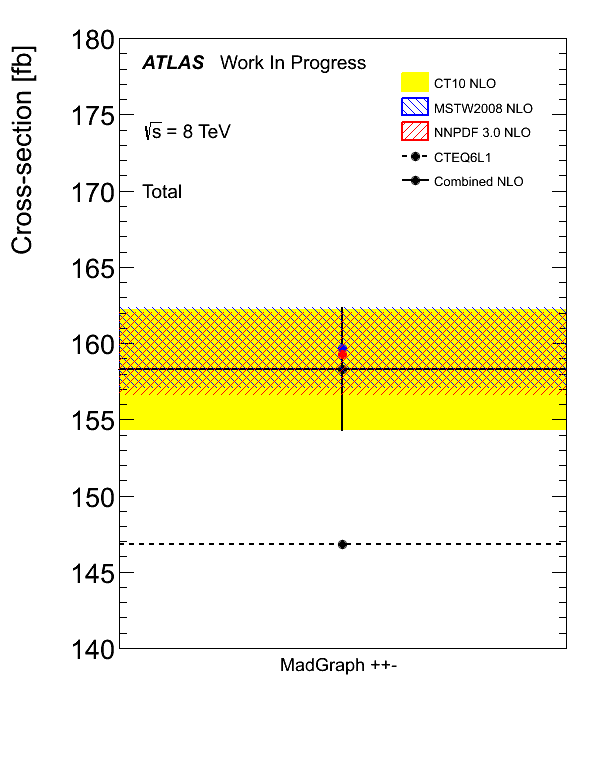
\includegraphics[width=.35\columnwidth]{figures/pdf/MADppm_total_cteq6l1.png}
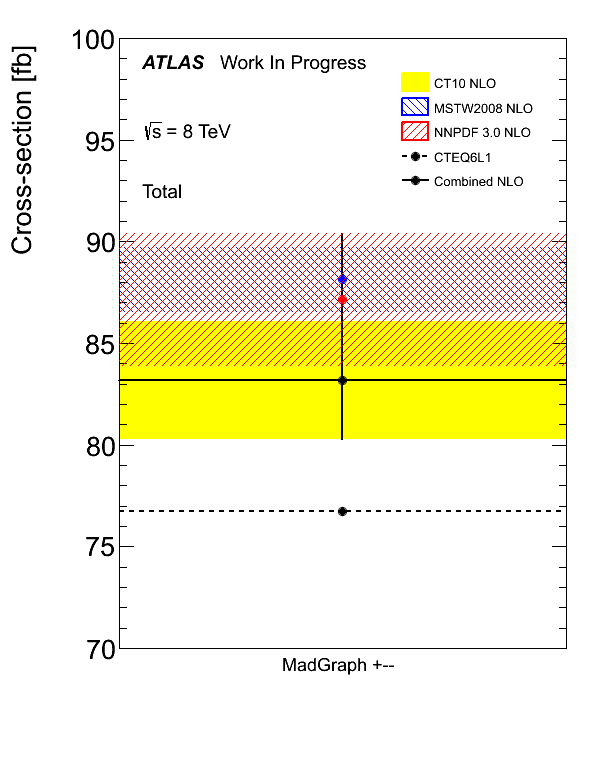
\includegraphics[width=.35\columnwidth]{figures/pdf/MADpmm_total_cteq6l1.png}
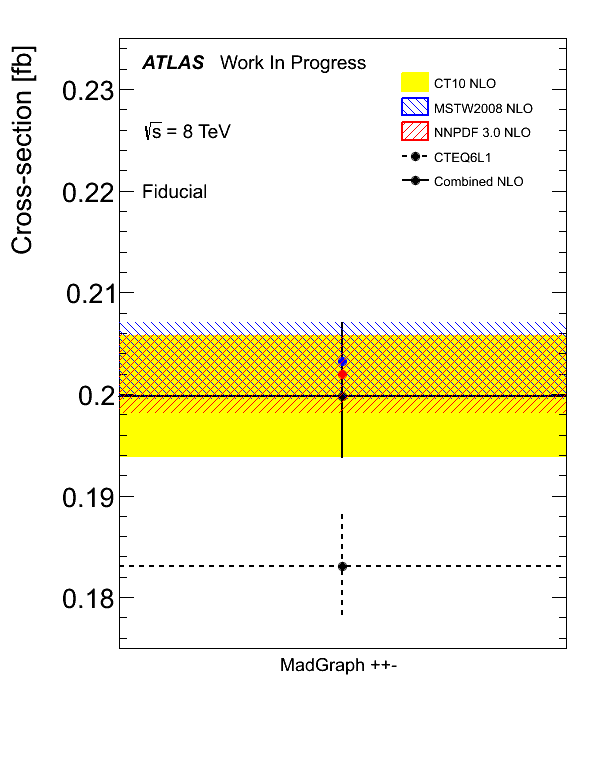
\includegraphics[width=.35\columnwidth]{figures/pdf/MADppm_fiducial_cteq6l1.png}
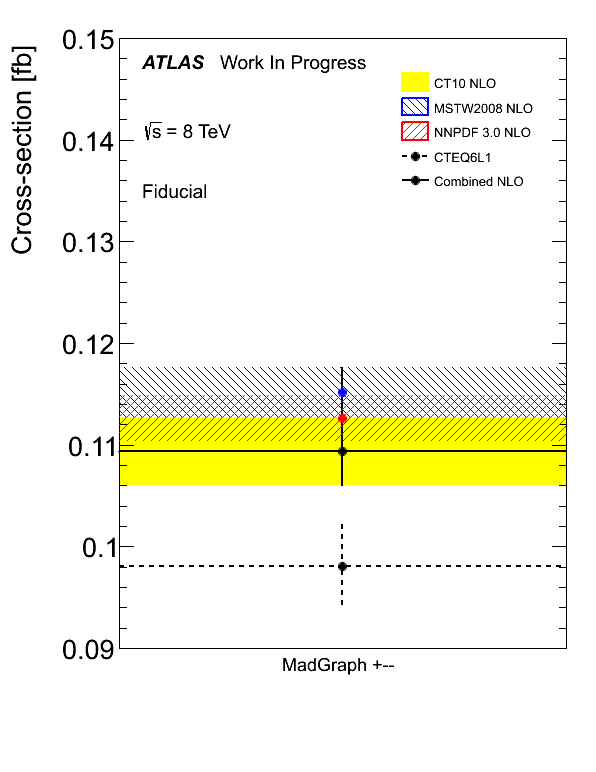
\includegraphics[width=.35\columnwidth]{figures/pdf/MADpmm_fiducial_cteq6l1.png}
\caption{The signal cross-sections for different PDFs along with their
uncertainties are shown on the {\sc MadGraph} $WWW$ signal samples
for the total $WWW$ phase space and branching fraction for
the $W^{+}W^{+}W^{-}$ (top left) and $W^{+}W^{-}W^{-}$ (top right)
charge modes
and in the fiducial region for $W^{+}W^{+}W^{-}$ (bottom left) 
and $W^{+}W^{-}W^{-}$ (bottom right).
The bands show the PDF uncertainty for CT10 NLO (solid yellow),
MSTW 2008 NLO (hashed blue), and NNPDF 3.0 NLO (hashed red). The
solid line shows the envelope of all uncertainty bands used as the final
PDF uncertainty estimate. The central value of CT10 NLO is taken as the
central value of the estimate.
The dashed-line shows the cross-section and 
statistical uncertainty for the CTEQ6L1
pdf sets used in the original generation step.}
\label{fig:signal_pdf_unc}
\end{figure}

\begin{table}[ht!]
\centering
\begin{tabular}{c|c|c}
\hline
 & \multicolumn{2}{c}{PDF Uncertainty}\\
 & $W^{+}W^{+}W^{-}$ & $W^{+}W^{-}W^{-}$ \\
\hline
\hline
Total & $+2.58\%~-2.51\%$ &  $+8.69\%~-3.47\%$ \\
Fiducial & $+3.64\%~-3.00\%$ & $+7.57\%~-3.08\%$ \\
\hline
\end{tabular}
\caption{Summary of PDF uncertainties estimated on NLO {\sc MadGraph} cross-sections
in both the fiducial and total phase space.}
\label{tab:pdfunc}
\end{table}

Uncertainties on the signal prediction mainly come from the choice of PDF, 
the inherent PDF uncertainty, and the renormalization and factorization
scales, as described in \sec\ref{sec:pdf}.
The uncertainty due to the choice of PDF is derived for the {\sc MadGraph} 
cross-sections following a modified version of the pdf4lhc
\cite{Botje:2011sn} recommendations.  The resulting 
uncertainty is shown separately for the two different charge modes
in both the fiducial and the inclusive phase
space in Table~\ref{tab:pdfunc}.
The uncertainty is determined by comparing three different PDFs:
CT10 NLO~\cite{Lai:2010vv}, MSTW2008 NLO~\cite{Martin:2009iq}, 
and NNPDF 3.0 NLO~\cite{Ball:2014uwa}. 
This comparison is presented in \fig\ref{fig:signal_pdf_unc}.  
Symmetric 68\% CL uncertainties 
are determined for CT10 NLO and MSTW 2008 NLO using the 68\% CL 
set provided for MSTW directly and the 90\%CL set for CT10 after
scaling down by 
a factor of 1.645 in order to approximate a 68 \% CL uncertainty. 
The uncertainty of the NNPDF 3.0 NLO PDF set is 
determined by using the standard deviation of the distribution 
of 101 MC PDFs provided in the PDF set; the nominal value is taken
from the mean of the same PDFs.  
The CT10 NLO PDF central value is used as the nominal 
value of the final estimate.
The final PDF uncertainty on that estimate is
taken as the envelope of the uncertainty bands for all three PDF sets.  



The uncertainty on the factorization and renormalization scales are 
determined by varying each of them independently up or down by 
a factor of two. 
The effect of these variations on the cross-sections
as compared to the nominal
are shown separately for the two different charge 
modes in \tab~\ref{tab:scaleVariation}.
The symmetric uncertainty is then determined by taking the maximum 
variation for each charge mode, 
namely, 2.62\% for $W^+W^+W^-$ and 2.53\% for $W^-W^+W^-$. 

\begin{table}[ht!]
    \centering
\begin{tabular}{cc|ccc}
\hline
& \backslashbox{$\mu_F$}{$\mu_R$}     & $\frac{1}{2}M_{WWW}$ & $M_{WWW}$ &  $2M_{WWW}$ \\
\cline{2-5}
\multirow{3}{*}{\Wp\Wp\Wm} &$\frac{1}{2}M_{WWW}$ & 2.62\% & -0.14\% & -2.11\% \\
%\cline{2-5}
&$M_{WWW}$ & 2.13\% & 0 & -2.41\% \\
%\cline{2-5}
&$2M_{WWW}$ & 1.56\% & 0.24\% & -2.42\% \\
\hline
\hline
& \backslashbox{$\mu_F$}{$\mu_R$}     & $\frac{1}{2}M_{WWW}$ & $M_{WWW}$ &  $2M_{WWW}$ \\
\cline{2-5}
\multirow{3}{*}{\Wm\Wp\Wm} &$\frac{1}{2}M_{WWW}$ & 1.91\% & 1.38\% & -2.00\% \\
%\cline{2-5}
&$M_{WWW}$ & 1.61\% & 0 & -2.53\% \\
%\cline{2-5}
&$2M_{WWW}$ & 1.25\% & -1.05\% & -2.12\% \\
\hline
\end{tabular}
\caption{The relative variation of the NLO cross sections corresponding 
to different choices of factorization and renormalization 
scales for the \Wp\Wp\Wm and \Wm\Wp\Wm  processes. }
\label{tab:scaleVariation}
\end{table}

The signal cross-sections and uncertainties are thus determined to be 
\begin{equation}
\sigma^{\textrm{Total}}_{\textrm{Theory}}= 241.47\pm0.13 ~(\textrm{Stat.}) ~^{+10.33}_{-6.08} ~(\textrm{PDF}) ~\pm 6.3 ~(\textrm{Scale}) ~\textrm{fb} %uncertainty?
\end{equation}
for the inclusive \xsec and
\begin{equation}
\label{eq:fiducial_theory}
\sigma^{\textrm{Fiducial}}_{\textrm{Theory}}= 309.2\pm7.2 ~(\textrm{Stat.}) ~^{+15.05}_{-8.36} ~(\textrm{PDF}) ~\pm 8.0 ~(\textrm{Scale}) ~\textrm{ab} %uncertainty?
\end{equation}
for the fiducial cross-section.


%should i include this
%The analysis considers events with three leptons ($e$ or $\mu$) in the final state. The contributions from events in which $W$ bosons decay to $\tau$'s, and the $\tau$'s sequentially decay to $e$ or $\mu$ should be included and is expected to be 40\% of total yield of the 3-lepton final state.  


\subsubsection{aQGC signal}
\label{sec:aqgc_signal}

MC samples of the aQGC signal processes described in \sec\ref{sec:eft}
have been generated using \vbfnlo at NLO in QCD.  (but don't we use LO?)
The cross-sections for the aQGC signal depend on the values
of the couplings $f_{s,0}$ and $f_{s,1}$. MC samples have 
been generated for a grid of points in the $f_{s,0}$ vs $f_{s,1}$ space
and their cross-sections are shown in \fig\ref{fig:aqgc_total_xsec_ununitarized_3l}. %histogram of cross-sections

\begin{figure}[ht!]
\centering
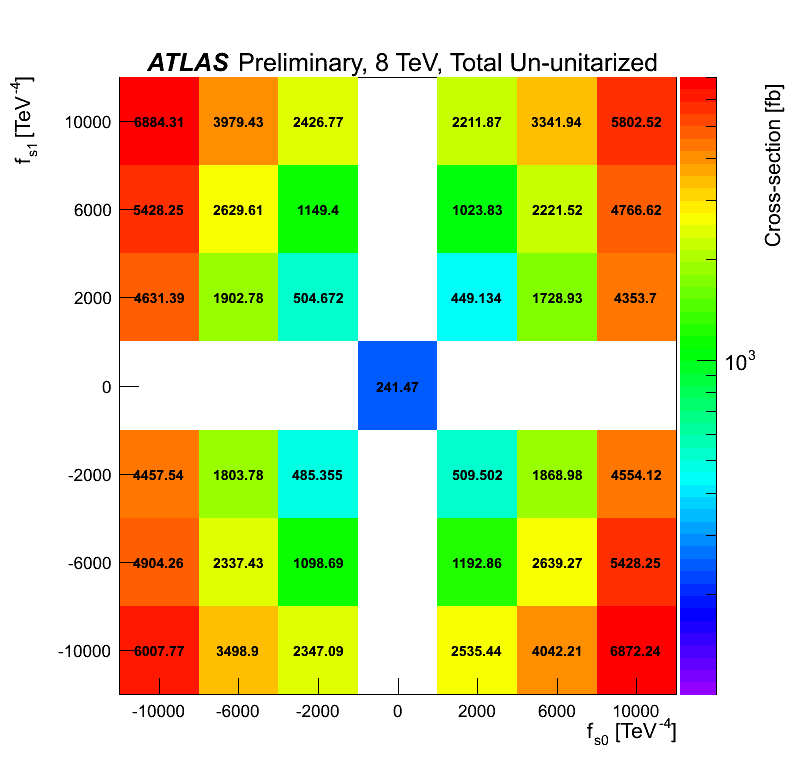
\includegraphics[width=.8\textwidth]{figures/aQGC/total_xsec/www_3l_aqgc_total_ununitarized_noratio.png}
\caption{Total cross-section for non-unitarized aQGC signal samples as a function of $f_{s,0}$ vs $f_{s,1}$.
The total SM cross-section is shown at $f_{s,0}=f_{s,1}=0$ for comparison.}
\label{fig:aqgc_total_xsec_ununitarized_3l}
\end{figure}

The issues of unitarity violation \sec\ref{sec:eft} are taken
into account using a form factor like in \eqn\eqref{eq:form_factor}.
The choices of the exponent, $n$, and form factor scale, $\Lambda$, 
are somewhat ad-hoc. Furthermore, a complete study of the unitarity
behavior of this process has never been performed, so there are not
currently detailed prescriptions on what to choose. 
However, based on discussions with the authors of \vbfnlo, who
are at the moment trying to perform these studies, an exponent
of $n=1$ is expected to be sufficient to achieve unitarity 
for this process.  As for the choice of $\Lambda$, we have
chosen to look at a few different values, which cover a wide
range but which should follow a smooth interpolation. 
This has the advantage of providing information about the
sensitivity to the form factor that can be interpreted 
by theorists as they see fit. Dedicated MC samples
are generated with the unitarization applied for values
of $\Lambda =$ 500~\GeV, 1000~\GeV, 2000~\GeV, and 3000~\GeV.
The cross-sections for each of these unitarization cases
are shown in \fig\ref{fig:aqgc_total_xsec_unitarized_3l}.

\begin{figure}[ht!]
\centering
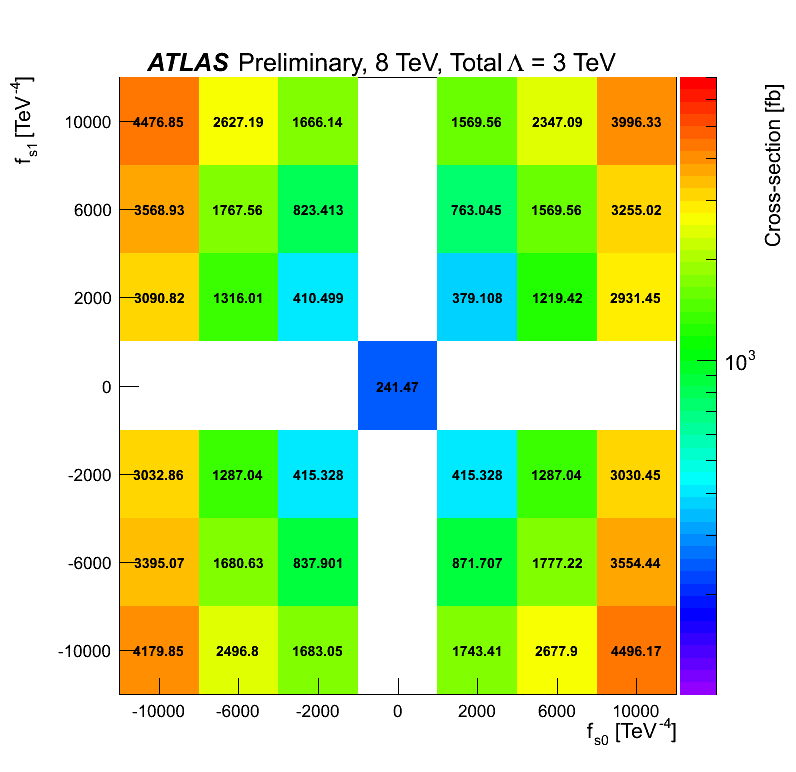
\includegraphics[width=.45\textwidth]{figures/aQGC/total_xsec/www_3l_aqgc_total_3TeV_noratio.png}
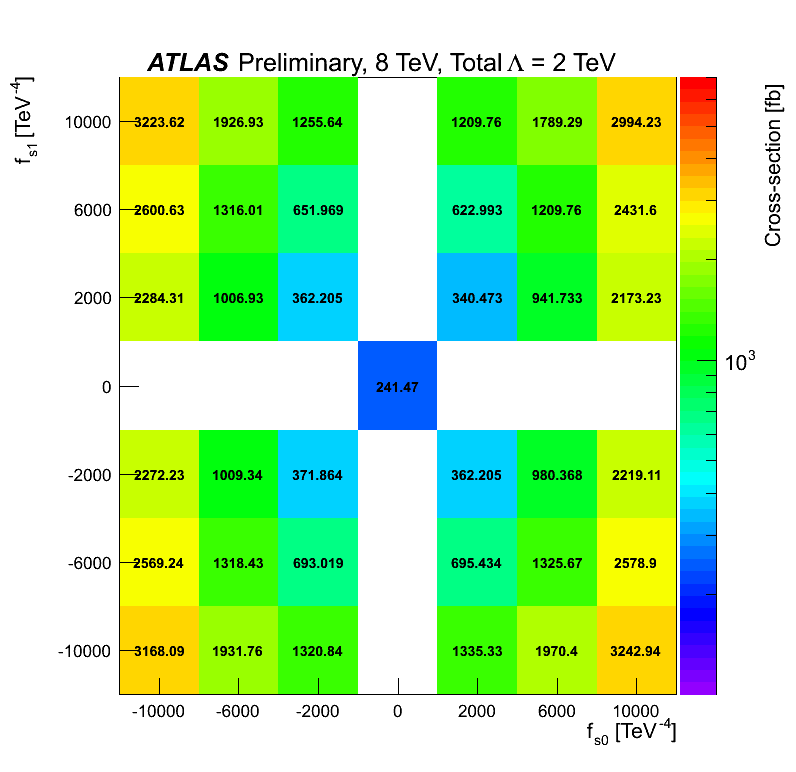
\includegraphics[width=.45\textwidth]{figures/aQGC/total_xsec/www_3l_aqgc_total_2TeV_noratio.png}
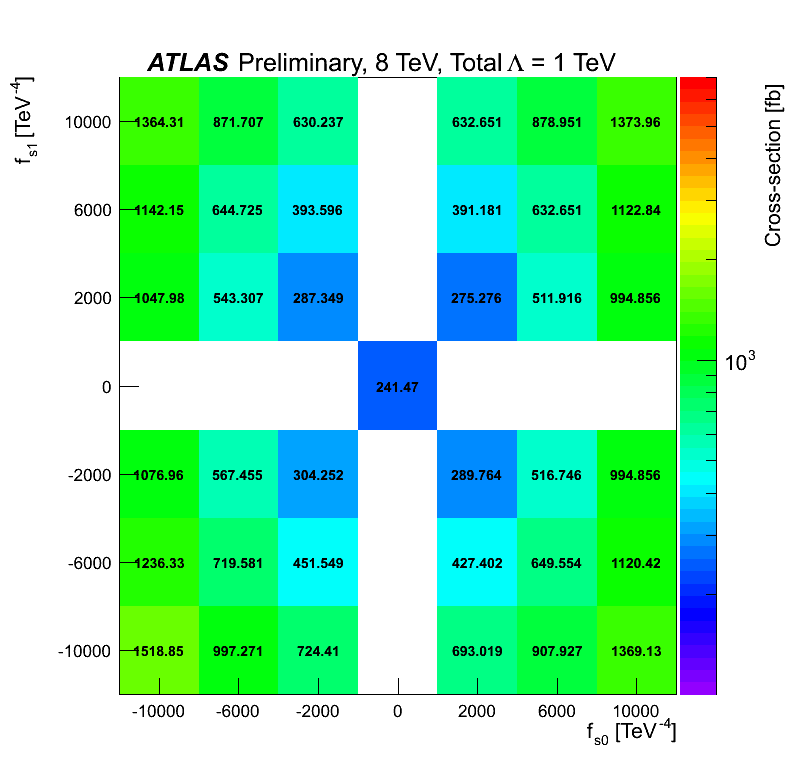
\includegraphics[width=.45\textwidth]{figures/aQGC/total_xsec/www_3l_aqgc_total_1TeV_noratio.png}
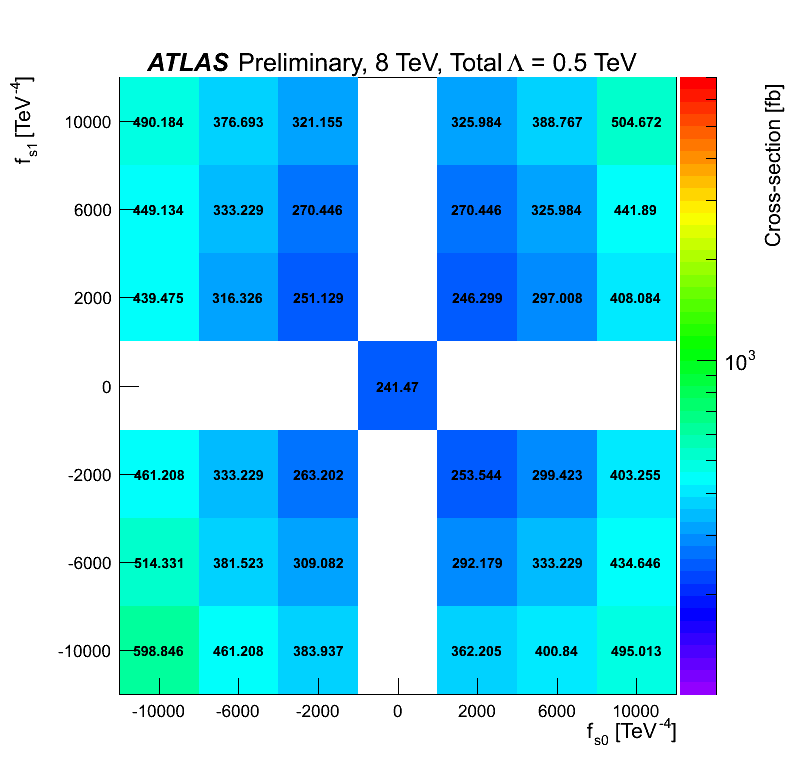
\includegraphics[width=.45\textwidth]{figures/aQGC/total_xsec/www_3l_aqgc_total_p5TeV_noratio.png}
\caption{Total cross-section for unitarized aQGC signal samples as a function of $f_{s,0}$ vs $f_{s,1}$.
Four different values of the unitarization scale, $\Lambda$, are chosen: 3~\TeV~(Top Left),
2~\TeV~(Top Right), 1~\TeV~(Bottom Left), and 0.5~\TeV~(Bottom Right).
The total SM cross-section is shown at $f_{s,0}=f_{s,1}=0$ for comparison.}
\label{fig:aqgc_total_xsec_unitarized_3l}
\end{figure}
























\newpage

\subsubsection{Backgrounds samples}
\label{sec:subsection_datasets_MC}

Only processes containing 3 or more prompt
leptons ($WZ$, $ZZ$, $t\bar{t}V$, $VVV$), or 2 leptons and an 
isolated photon ($Z+\gamma$) are estimated using MC simulation 
samples in this analysis. The other processes are estimated from 
data as this will be explained in Section~\ref{sec:backgrounds_estimation}. 
The samples listed in this section and containing less than 3 prompt leptons 
have been used for preliminary or dedicated studies, but are not used for 
the determination of the final results. The MC samples are pass through the 
GEANT4~\cite{Agostinelli:2002hh} simulation~\cite{Aad:2010ah} of the ATLAS 
detector and reconstructed in the same way as the data.

The diboson and triboson samples are listed in Table~\ref{tab:sample_bkg_dibosons}. The triboson samples other than the signal, \textit{ie}: $ZWW^{*}$ and $ZZZ^{*}$ were generated using the MadGraph~\cite{Alwall_madgraph} generator, hadronized through the Pythia6~\cite{PYTHIA} parton shower, with the AUET2B~\cite{ATL-PHYS-PUB-2011-009} tunes and the CTEQ6L1~\cite{Pumplin:2002vw} PDF set. The $Z\gamma$ samples were generated with the Sherpa~\cite{sherpa} generator and the CT10~\cite{Guzzi:2011sv} PDF set. The $W\gamma$ samples were generated with the AlpGen~\cite{ALPGEN} generator, hadronized through JIMMY~\cite{Jimmy}, with the AUET2C~\cite{ATL-PHYS-PUB-2011-009} tunes and the CTEQ6L1 PDF set. Other diboson samples ($WW$, $WZ$, $ZZ$) were obtained using the Powheg~\cite{Alioli:2008gx,Nason:2004rx,Frixione:2007vw,Alioli:2010xd} generator, hadronized through the Pythia8~\cite{Sjostrand:2007gs} parton shower, with the AU2~\cite{atlasmctunes} tunes and the CT10 PDF set. Dedicated high-stat $WZ$ and $ZZ$ samples were generated to increase the statistics in all the signal region used in this analysis. They were obtained requesting the presence of 3 leptons with $\pt>7~\GeV$.

The dibosons samples where the production is due to loop induced process or Double Parton Scattering (DPS) processes are summarized in Table~\ref{tab:sample_bkg_dibosons_gg2DPI}. The loop induced processes were generated using the gg2ZZ~\cite{Binoth:2008pr} and gg2WW~\cite{Binoth:2006mf} generators, hadronized using JIMMY, with the AU2 tunes and the CT10 PDF set. The DPS processes were generated with the AU2 tunes and the CTEQ6L1 PDF set. The cross section of these processes have been evaluated for the ATLAS same sign WW analysis~\cite{Aad:2014zda}, as this will be explained in Section~\ref{sec:bkg_DPS}.

Single boson processes are summarized in Table~\ref{tab:sample_bkg_Zjets} for the $Z+$jets samples and in Table~\ref{tab:sample_bkg_wjets} for the $W+$jets samples. The $Z+$jets samples were generated with the Sherpa generator and the CT10 PDF set. Low mass Drell-Yan samples were not simluated using the GEANT4 simulation, but with the AF2 simulation, however dedicated scale factors are applied for these samples, when they are used, in the analysis. The $W+$jets samples were generated with the AlpGen generator, hadronized through JIMMY, with the AUET2C tunes and the CTEQ6L1 PDF set.

Samples containing top quarks are summarized in Table~\ref{tab:sample_bkg_top}. $t\bar{t}$ events were generated using the MCatNLO\cite{MCatNLO} generator, hadronized through JIMMY with the CT10 PDF set. Single top samples in the s-channel and in the $Wt$ channel were generated using MCatNLO hadronized through JIMMY with the CT10 PDF set. Single top samples in the t-channel were generated using AcerMC\cite{Kersevan:2004yg}, hadronized using PYTHIA6 with the AUET2B tunes and the CTEQ6L1 PDF set. Finally $t\bar{t}V$ processes were generated using the MadGraph generator, hadronized through the Pythia6 parton shower, with the AUET2B tunes and the CTEQ6L1PDF set.


 % the $Z+jets$ samples in Table~\ref{tab:sample_bkg_Zjets}, the $W+jets$ in Table~\ref{tab:sample_bkg_wjets}, and samples containing top quarks in Table~\ref{tab:sample_bkg_top}.

When $Z+$jets and $Z+\gamma$ samples are used simultaneously, an overlap removal procedure must be used to avoid double counting of FSR events. Events containing an FSR photon with $E_{T}>10~\GeV$ are explicitely vetoed out from the $Z+$jets sample. The algorithm used is the same as what was developped in the $8~\TeV$ ATLAS $WZ$ analysis~\cite{Anger:1663539}.


\begin{table}[ht!]
  \centering
  \begin{footnotesize}
\begin{tabular}{c|c|c|c|c|c|c}
\hline
    &  &  & Cross-Section &  & Event filter  \\
  Sample  & Generator & Sample type & [pb] & k-factor &  efficiency  & used in signal region\\
\hline \hline
167007 & MadGraphPythia & ZWWStar lllnulnu  &  0.0015546  &  1  &  1 & Yes \\
167008 & MadGraphPythia & ZZZStar nunullll  &  0.00033239  &  1  &  1 & Yes \\
145161 & Sherpa & eegammaPt10  &  32.26  &  1  &  1 & Yes \\
145162 & Sherpa & mumugammaPt10  &  32.317  &  1  &  1 & Yes \\
%146430 & AlpgenJimmy & Wgamma Np0 & 230.09 & 1.15 & 1 & No \\
%146431 & AlpgenJimmy & Wgamma Np1 & 59.343 & 1.15 & 1 & No \\
%146432 & AlpgenJimmy & Wgamma Np2 & 21.469 & 1.15 & 1 & No \\
%146433 & AlpgenJimmy & Wgamma Np3 & 7.1032 & 1.15 & 1 & No \\
%146434 & AlpgenJimmy & Wgamma Np4 & 2.1224 & 1.15 & 1 & No \\
%146435 & AlpgenJimmy & Wgamma Np5 & 0.46612 & 1.15 & 1 & No \\
146436 & AlpgenJimmy & Wgamma Np0 & 229.88 & 1.15 & 0.31372 & No \\
146437 & AlpgenJimmy & Wgamma Np1 & 59.518 & 1.15 & 0.44871 & No \\
146438 & AlpgenJimmy & Wgamma Np2 & 21.39  & 1.15 & 0.54461 & No \\
146439 & AlpgenJimmy & Wgamma Np3 & 7.1203 & 1.15 & 0.62974 & No \\
126928 & PowhegPythia8& WpWm ee  &  0.62  &  1.0  &  1 & No  \\
126929 & PowhegPythia8& WpWm me  &  0.62  &  1.0  &  1 & No  \\
126930 & PowhegPythia8& WpWm te  &  0.62  &  1.0  &  1 & No  \\
126931 & PowhegPythia8& WpWm em  &  0.62  &  1.0  &  1 & No \\
126932 & PowhegPythia8& WpWm mm  &  0.62  &  1.0  &  1 & No \\
126933 & PowhegPythia8& WpWm tm  &  0.62  &  1.0  &  1 & No \\
126934 & PowhegPythia8& WpWm et  &  0.62  &  1.0  &  1 & No \\
126935 & PowhegPythia8& WpWm mt  &  0.62  &  1.0  &  1 & No \\
126936 & PowhegPythia8& WpWm tt  &  0.62  &  1.0  &  1 & No \\

185813 & PowhegPythia8& ZZ 4e mll4 TriLeptonFilter & 0.07677 & 1 & 0.57204 & Yes \\
185814 & PowhegPythia8& ZZ 2e2mu mll4 TriLeptonFilter & 0.1757 & 1 & 0.49893 & Yes \\
185815 & PowhegPythia8& ZZ 2e2tau mll4 TriLeptonFilter & 0.1757 & 1 & 0.086032 & Yes \\
185816 & PowhegPythia8& ZZ 4mu mll4 TriLeptonFilter & 0.07677 & 1 & 0.58293 & Yes \\
185817 & PowhegPythia8& ZZ 2mu2tau mll4 TriLeptonFilter & 0.1757 & 1 & 0.087166 & Yes \\
185818 & PowhegPythia8& ZZ 4tau mll4 TriLeptonFilter & 0.07677 & 1 & 0.0076557 & Yes \\

181471 & Sherpa & $ZZ*\rightarrow eeee$  $m_{Z,1} > 4$~GeV, $m_{Z,2} < 4$~GeV  & 2.8286 & 0.880 & 1.0 & No \\
181472 & Sherpa & $ZZ*\rightarrow ee\mu\mu$ $m_{Z,1} > 4$~GeV, $m_{Z,2} < 4$~GeV  & 2.34503 & 0.880 & 1.0 & No \\
181473 & Sherpa & $ZZ*\rightarrow ee\tau\tau$ $m_{Z,1} > 4$~GeV, $m_{Z,2} < 4$~GeV  & 1.59326 & 0.880 & 1.0 & No \\
181474 & Sherpa & $ZZ*\rightarrow \mu\mu ee$ $m_{Z,1} > 4$~GeV, $m_{Z,2} < 4$~GeV  & 0.48613 & 0.880 & 1.0 & No \\
181475 & Sherpa & $ZZ*\rightarrow \mu\mu\mu\mu$ $m_{Z,1} > 4$~GeV, $m_{Z,2} < 4$~GeV  & 0.50835 & 0.880 & 1.0 & No \\
181476 & Sherpa & $ZZ*\rightarrow \mu\mu\tau\tau$ $m_{Z,1} > 4$~GeV, $m_{Z,2} < 4$~GeV  & 0.42288 & 0.880 & 1.0 & No \\
181477 & Sherpa & $ZZ*\rightarrow \tau\tau ee$ $m_{Z,1} > 4$~GeV, $m_{Z,2} < 4$~GeV  & 0.00403 & 0.880 & 1.0 & No \\
181478 & Sherpa & $ZZ*\rightarrow \tau\tau\mu\mu$ $m_{Z,1} > 4$~GeV, $m_{Z,2} < 4$~GeV  & 0.00401 & 0.880 & 1.0 & No \\
181479 & Sherpa & $ZZ*\rightarrow \tau\tau\tau\tau$ $m_{Z,1} > 4$~GeV, $m_{Z,2} < 4$~GeV  & 0.00411 & 0.880 & 1.0 & No \\


% 126937 & PowhegPythia8& ZZ 4e mll4 2pt5  &  0.0735  &  1.0  &  0.90765 \\
% 126938 & PowhegPythia8& ZZ 2e2mu mll4 2pt5  &  0.1708  &  1.0  &  0.82724 \\
% 126939 & PowhegPythia8& ZZ 2e2tau mll4 2pt5  &  0.1708  &  1.0  &  0.58278 \\
% 126940 & PowhegPythia8& ZZ 4mu mll4 2pt5  &  0.0735  &  1.0  &  0.91241 \\
% 126941 & PowhegPythia8& ZZ 2mu2tau mll4 2pt5  &  0.1708  &  1.0  &  0.58725 \\
% 126942 & PowhegPythia8& ZZ 4tau mll4 2pt5  &  0.0735  &  1.0  &  0.10604 \\
126949 & PowhegPythia8& ZZllnunu ee mll4  &  0.168  &  1  &  1 & No \\
126950 & PowhegPythia8& ZZllnunu mm mll4  &  0.168  &  1  &  1 & No \\
126951 & PowhegPythia8& ZZllnunu tt mll4  &  0.168  &  1  &  1 & No \\
185795  &  PowhegPythia8 &  WmZ 3e mll0p25 TriLeptonFilter  &  0.9655  &  1  &  0.051928 & Yes \\
185796  &  PowhegPythia8 &  WmZ e2mu mll0p4614 TriLeptonFilter  &  0.6326  &  1  &  0.073874  & Yes \\
185797  &  PowhegPythia8 &  WmZ e2tau mll3p804 TriLeptonFilter  &  0.1125  &  1  &  0.012544  & Yes \\
185798  &  PowhegPythia8 &  WmZ mu2e mll0p25 TriLeptonFilter  &  0.9687  &  1  &  0.054302  & Yes \\
185799  &  PowhegPythia8 &  WmZ 3mu mll0p4614 TriLeptonFilter  &  0.6479  &  1  &  0.071268  & Yes \\
185800  &  PowhegPythia8 &  WmZ mu2tau mll3p804 TriLeptonFilter  &  0.1125  &  1  &  0.01258  & Yes \\
185801  &  PowhegPythia8 &  WmZ tau2e mll0p25 TriLeptonFilter  &  0.9687  &  1  &  0.012075  & Yes \\
185802  &  PowhegPythia8 &  WmZ tau2mu mll0p4614 TriLeptonFilter  &  0.6326  &  1  &  0.01664 & Yes \\
185803  &  PowhegPythia8 &  WmZ 3tau mll3p804 TriLeptonFilter  &  0.1108  &  1  &  0.0034037  & Yes \\
185804  &  PowhegPythia8 &  WpZ 3e mll0p25 TriLeptonFilter  &  1.416  &  1  &  0.053051 & Yes  \\
185805  &  PowhegPythia8 &  WpZ e2mu mll0p4614 TriLeptonFilter  &  0.9421  &  1  &  0.075904  & Yes \\
185806  &  PowhegPythia8 &  WpZ e2tau mll3p804 TriLeptonFilter  &  0.1755  &  1  &  0.013867 & Yes  \\
185807  &  PowhegPythia8 &  WpZ mu2e mll0p25 TriLeptonFilter  &  1.412  &  1  &  0.055296 & Yes  \\
185808  &  PowhegPythia8 &  WpZ 3mu mll0p4614 TriLeptonFilter  &  0.9572  &  1  &  0.073362 & Yes  \\
185809  &  PowhegPythia8 &  WpZ mu2tau mll3p804 TriLeptonFilter  &  0.1755  &  1  &  0.013891 & Yes \\
185810  &  PowhegPythia8 &  WpZ tau2e mll0p25 TriLeptonFilter  &  1.412  &  1  &  0.012105 & Yes  \\
185811  &  PowhegPythia8 &  WpZ tau2mu mll0p4614 TriLeptonFilter  &  0.9421  &  1  &  0.016718 & Yes  \\
185812  &  PowhegPythia8 &  WpZ 3tau mll3p804 TriLeptonFilter  &  0.172  &  1  &  0.0036427 & Yes  \\
% 129477 & PowhegPythia8& WZ Wm11Z11 mll0p250d0 2LeptonFilter5  &  1.407  &  1.0  &  0.29456 \\
% 129478 & PowhegPythia8& WZ Wm11Z13 mll0p4614d0 2LeptonFilter5  &  0.9382  &  1.0  &  0.35211 \\
% 129479 & PowhegPythia8& WZ Wm11Z15 mll3p804d0 2LeptonFilter5  &  0.1746  &  1.0  &  0.16682 \\
% 129480 & PowhegPythia8& WZ Wm13Z11 mll0p250d0 2LeptonFilter5  &  1.399  &  1.0  &  0.29351 \\
% 129481 & PowhegPythia8& WZ Wm13Z13 mll0p4614d0 2LeptonFilter5  &  0.9537  &  1.0  &  0.35132 \\
% 129482 & PowhegPythia8& WZ Wm13Z15 mll3p804d0 2LeptonFilter5  &  0.1746  &  1.0  &  0.16863 \\
% 129483 & PowhegPythia8& WZ Wm15Z11 mll0p250d0 2LeptonFilter5  &  1.399  &  1.0  &  0.14289 \\
% 129484 & PowhegPythia8& WZ Wm15Z13 mll0p4614d0 2LeptonFilter5  &  0.9382  &  1.0  &  0.18256 \\
% 129485 & PowhegPythia8& WZ Wm15Z15 mll3p804d0 2LeptonFilter5  &  0.1719  &  1.0  &  0.058517 \\
% 129486 & PowhegPythia8& WZ W11Z11 mll0p250d0 2LeptonFilter5  &  0.9795  &  1.0  &  0.29694 \\
% 129487 & PowhegPythia8& WZ W11Z13 mll0p4614d0 2LeptonFilter5  &  0.639  &  1.0  &  0.35302 \\
% 129488 & PowhegPythia8& WZ W11Z15 mll3p804d0 2LeptonFilter5  &  0.1125  &  1.0  &  0.15969 \\
% 129489 & PowhegPythia8& WZ W13Z11 mll0p250d0 2LeptonFilter5  &  0.9359  &  1.0  &  0.29766 \\
% 129490 & PowhegPythia8& WZ W13Z13 mll0p4614d0 2LeptonFilter5  &  0.6488  &  1.0  &  0.35414 \\
% 129491 & PowhegPythia8& WZ W13Z15 mll3p804d0 2LeptonFilter5  &  0.1125  &  1.0  &  0.16023 \\
% 129492 & PowhegPythia8& WZ W15Z11 mll0p250d0 2LeptonFilter5  &  0.9359  &  1.0  &  0.14803 \\
% 129493 & PowhegPythia8& WZ W15Z13 mll0p4614d0 2LeptonFilter5  &  0.639  &  1.0  &  0.18657 \\
% 129494 & PowhegPythia8& WZ W15Z15 mll3p804d0 2LeptonFilter5  &  0.1107  &  1.0  &  0.056651 \\
\hline 
\end{tabular}
\end{footnotesize}
\caption{List of diboson samples used in the analysis. 
For the three lepton signal regions, it is indicated for each
sample whether or not the sample is used.  If not, it is replaced
by a data-driven fake estimate described in Section~\ref{sec:fakebg}.
All samples are used in dilepton control regions.
}
\label{tab:sample_bkg_dibosons}
\end{table}


\begin{table}[ht!]
  \centering
  \begin{footnotesize}
\begin{tabular}{c|c|c|c|c|c|c}
\hline
    &  &  & Cross-Section &  & Event filter  \\
  Sample  & Generator & Sample type & [pb] & k-factor &  efficiency  & used in signal region\\
\hline \hline
116600 & gg2ZZJimmy & ZZ4lep & 0.00459 & 1 & 1 & Yes \\
116601 & gg2ZZJimmy & ZZ4e & 0.000675 & 1 & 1  & Yes \\
116602 & gg2ZZJimmy & ZZ4mu & 0.000675 & 1 & 1  & Yes \\
116603 & gg2ZZJimmy & ZZ2e2mu & 0.00134539 & 1 & 1 & Yes  \\
169471 & gg2wwJimmy & WpWmenuenu & 0.017 & 1 & 1   & No \\
169472 & gg2wwJimmy & WpWmenumunu & 0.017 & 1 & 1  & No  \\
169473 & gg2wwJimmy & WpWmenutaunu & 0.017 & 1 & 1 & No  \\
169474 & gg2wwJimmy & WpWmmunumunu & 0.017 & 1 & 1 & No   \\
169475 & gg2wwJimmy & WpWmmunuenu & 0.017 & 1 & 1  & No  \\
169476 & gg2wwJimmy & WpWmmunutaunu & 0.017 & 1 & 1  & No  \\
169477 & gg2wwJimmy & WpWmtaunutaunu & 0.017 & 1 & 1 & No   \\
169478 & gg2wwJimmy & WpWmtaunuenu & 0.017 & 1 & 1   & No \\
169479 & gg2wwJimmy & WpWmtaunumunu & 0.017 & 1 & 1  & No  \\
147280 & Pythia8 & DPI W W 2l & 0.0258 & 1 & 0.48 & Yes  \\
147281 & Pythia8 & DPI W W 2l2j & 0.0258 & 1 & 0.0752 & Yes  \\
147282 & Pythia8 & DPI W Z 2l & 0.139 & 1 & 0.0539 & Yes  \\
147283 & Pythia8 & DPI W Z 2l2j & 0.139 & 1 & 0.00873 & Yes  \\
147284 & Pythia8 & DPI W gamma 1l1gm & 9.86 & 1 & 0.159 & Yes  \\
147285 & Pythia8 & DPI Z Z 2l & 0.213 & 1 & 0.0547 & Yes  \\
147286 & Pythia8 & DPI Z Z 2l2j & 0.213 & 1 & 0.00457 & Yes  \\
147287 & Pythia8 & DPI Z gamma 1l1gm & 26.5 & 1 & 0.012 & Yes  \\
147288 & Pythia8 & DPI WZ dijet 2l2j & 1.43 & 1 & 0.102 & Yes  \\
147289 & Pythia8 & DPI ZZ dijet 2l2j & 1.86 & 1 & 0.0422 & Yes  \\
147290 & Pythia8 & DPI W diphoton 1l2gm & 0.012 & 1 & 0.0632 & Yes  \\
147291 & Pythia8 & DPI Zll diphoton 1l2gm & 0.00581 & 1 & 0.0259 & Yes  \\
147292 & Pythia8 & DPI Zvv diphoton 2gm & 0.00221 & 1 & 0.0898 & Yes  \\
147293 & Pythia8 & DPI gamma gamma 2gm & 943 & 1 & 0.00422 & Yes  \\
\hline 
\end{tabular}
\end{footnotesize}
\caption{List of loop induced, or DPI, diboson samples used in the analysis.
For the three lepton signal regions, it is indicated for each
sample whether or not the sample is used.  If not, it is replaced
by a data-driven fake estimate described in Section~\ref{sec:fakebg}.
All samples are used in dilepton control regions.
}
\label{tab:sample_bkg_dibosons_gg2DPI}
\end{table}




\begin{table}[ht!]
  \centering
  \begin{footnotesize}
  
\begin{tabular}{c|c|c|c|c|c|c}
\hline
    &  &  & Cross-Section &  & Event filter  \\
  Sample  & Generator & Sample type & [pb] & k-factor &  efficiency  & used in signal region\\
\hline \hline
147770 & Sherpa & Zee  				&  1241.2  &  1  & 1 & No \\
147771 & Sherpa & Zmumu  			&  1241.2  &  1  & 1 & No \\
147772 & Sherpa & Ztautau  			&  1241.2  &  1  & 1 & No \\
173041 & Sherpa & DYeeM08to15 		& 92.148	& 1  & 1 & No \\
173042 & Sherpa & DYeeM015to40 		& 279.06	& 1  & 1 & No \\
173043 & Sherpa & DYmumuM015to40 	& 	92.097  & 1  & 1 & No \\
173044 & Sherpa & DYmumuM015to40 	& 	279.31  & 1  & 1 & No \\
173045 & Sherpa & DYtautauM015to40 	& 92.121	& 1  & 1 & No \\
173046 & Sherpa & DYtautauM015to40 	& 279.26	& 1  & 1 & No \\

% 146830 & AlpgenJimmy & ZeeNp0Excl Mll10to60  &  3477.2  &  1.19  &  1 \\
% 146831 & AlpgenJimmy & ZeeNp1Excl Mll10to60  &  108.8  &  1.19  &  1 \\
% 146832 & AlpgenJimmy & ZeeNp2Excl Mll10to60  &  52.767  &  1.19  &  1 \\
% 14683 & AlpgenJimmy & ZeeNp3Excl Mll10to60  &  11.297  &  1.19  &  1 \\
% 14683 & AlpgenJimmy & ZeeNp4Excl Mll10to60  &  2.5836  &  1.19  &  1 \\
% 14683 & AlpgenJimmy & ZeeNp5Incl Mll10to60  &  0.69267  &  1.19  &  1 \\
% 14684 & AlpgenJimmy & ZmumuNp0Excl Mll10to60  &  3477.1  &  1.19  &  1 \\
% 14684 & AlpgenJimmy & ZmumuNp1Excl Mll10to60  &  108.75  &  1.19  &  1 \\
% 14684 & AlpgenJimmy & ZmumuNp2Excl Mll10to60  &  52.741  &  1.19  &  1 \\
% 14684 & AlpgenJimmy & ZmumuNp3Excl Mll10to60  &  11.241  &  1.19  &  1 \\
% 14684 & AlpgenJimmy & ZmumuNp4Excl Mll10to60  &  2.6005  &  1.19  &  1 \\
% 14684 & AlpgenJimmy & ZmumuNp5Incl Mll10to60  &  0.69373  &  1.19  &  1 \\
% 14685 & AlpgenJimmy & ZtautauNp0Excl Mll10to60  &  3477.1  &  1.19  &  1 \\
% 14685 & AlpgenJimmy & ZtautauNp1Excl Mll10to60  &  108.74  &  1.19  &  1 \\
% 14685 & AlpgenJimmy & ZtautauNp2Excl Mll10to60  &  52.732  &  1.19  &  1 \\
% 14685 & AlpgenJimmy & ZtautauNp3Excl Mll10to60  &  11.326  &  1.19  &  1 \\
% 14685 & AlpgenJimmy & ZtautauNp4Excl Mll10to60  &  2.592  &  1.19  &  1 \\
% 14685 & AlpgenJimmy & ZtautauNp5Incl Mll10to60  &  0.6929  &  1.19  &  1 \\
% 10930 & AlpgenJimmy & ZeebbNp0  &  8.3777  &  1.23  &  1 \\
% 10930 & AlpgenJimmy & ZeebbNp1  &  3.2529  &  1.23  &  1 \\
% 10930 & AlpgenJimmy & ZeebbNp2  &  1.1902  &  1.23  &  1 \\
% 10930 & AlpgenJimmy & ZeebbNp3  &  0.50278  &  1.23  &  1 \\
% 12641 & AlpgenJimmy & ZeeccNp0  &  15.654  &  1.23  &  1 \\
% 12641 & AlpgenJimmy & ZeeccNp1  &  6.8946  &  1.23  &  1 \\
% 12641 & AlpgenJimmy & ZeeccNp2  &  2.9204  &  1.23  &  1 \\
% 12641 & AlpgenJimmy & ZeeccNp3  &  1.1411  &  1.23  &  1 \\
% 10930 & AlpgenJimmy & ZmumubbNp0  &  8.3742  &  1.23  &  1 \\
% 10930 & AlpgenJimmy & ZmumubbNp1  &  3.254  &  1.23  &  1 \\
% 10930 & AlpgenJimmy & ZmumubbNp2  &  1.181  &  1.23  &  1 \\
% 10930 & AlpgenJimmy & ZmumubbNp3  &  0.50669  &  1.23  &  1 \\
% 12641 & AlpgenJimmy & ZmumuccNp0  &  15.649  &  1.23  &  1 \\
% 12641 & AlpgenJimmy & ZmumuccNp1  &  6.893  &  1.23  &  1 \\
% 12642 & AlpgenJimmy & ZmumuccNp2  &  2.9176  &  1.23  &  1 \\
% 12642 & AlpgenJimmy & ZmumuccNp3  &  1.1377  &  1.23  &  1 \\
% 10931 & AlpgenJimmy & ZtautaubbNp0  &  8.3757  &  1.23  &  1 \\
% 10931 & AlpgenJimmy & ZtautaubbNp1  &  3.2427  &  1.23  &  1 \\
% 10931 & AlpgenJimmy & ZtautaubbNp2  &  1.1938  &  1.23  &  1 \\
% 10931 & AlpgenJimmy & ZtautaubbNp3  &  0.49791  &  1.23  &  1 \\
% 11770 & AlpgenJimmy & ZtautauccNp0  &  15.652  &  1.23  &  1 \\
% 11770 & AlpgenJimmy & ZtautauccNp1  &  6.8979  &  1.23  &  1 \\
% 11770 & AlpgenJimmy & ZtautauccNp2  &  2.91  &  1.23  &  1 \\
% 11770 & AlpgenJimmy & ZtautauccNp3  &  1.134  &  1.23  &  1 \\
\hline 
\end{tabular}
  \end{footnotesize}

\caption{List of $Z+jets$ samples used in the analysis. 
For the three lepton signal regions, it is indicated for each
sample whether or not the sample is used.  If not, it is replaced
by a data-driven fake estimate described in Section~\ref{sec:fakebg}.
All samples are used in dilepton control regions.
}
\label{tab:sample_bkg_Zjets}
\end{table}

\begin{table}[ht!]
\centering
  \begin{footnotesize}

\begin{tabular}{c|c|c|c|c|c|c}
\hline
    &  &  & Cross-Section &  & Event filter  \\
  Sample  & Generator & Sample type & [pb] & k-factor &  efficiency  & used in signal region\\
\hline \hline
107680 & AlpgenJimmy & WenuNp0  &  8037.1  &  1.19  &  1  & No \\
107681 & AlpgenJimmy & WenuNp1  &  1579.2  &  1.19  &  1  & No \\
107682 & AlpgenJimmy & WenuNp2  &  477.2   &  1.19  &  1  & No \\
107683 & AlpgenJimmy & WenuNp3  &  133.93  &  1.19  &  1  & No \\
107684 & AlpgenJimmy & WenuNp4  &  35.622  &  1.19  &  1  & No \\
107685 & AlpgenJimmy & WenuNp5  &  10.553  &  1.19  &  1  & No \\
107690 & AlpgenJimmy & WmunuNp0  &  8040   &  1.19  &  1  & No \\
107691 & AlpgenJimmy & WmunuNp1  &  1580.3 &  1.19  &  1  & No \\
107692 & AlpgenJimmy & WmunuNp2  &  477.5  &  1.19  &  1  & No \\
107693 & AlpgenJimmy & WmunuNp3  &  133.94 &  1.19  &  1  & No \\
107694 & AlpgenJimmy & WmunuNp4  &  35.636 &  1.19  &  1  & No \\
107695 & AlpgenJimmy & WmunuNp5  &  10.571 &  1.19  &  1  & No \\
107700 & AlpgenJimmy & WtaunuNp0  &  8035.8&  1.19  &  1  & No \\
107701 & AlpgenJimmy & WtaunuNp1  &  1579.8 &  1.19  &  1  & No \\
107702 & AlpgenJimmy & WtaunuNp2  &  477.55 &  1.19  &  1  & No \\
107703 & AlpgenJimmy & WtaunuNp3  &  133.79 &  1.19  &  1  & No \\
107704 & AlpgenJimmy & WtaunuNp4  &  35.583 &  1.19  &  1  & No \\
107705 & AlpgenJimmy & WtaunuNp5  &  10.54  &  1.19  &  1  & No \\
\hline 
\end{tabular}
  \end{footnotesize}

\caption{List of $W+jets$ used in the analysis.  
For the three lepton signal regions, it is indicated for each
sample whether or not the sample is used.  If not, it is replaced
by a data-driven fake estimate described in Section~\ref{sec:fakebg}.
All samples are used in dilepton control regions.
}
\label{tab:sample_bkg_wjets}
\end{table}


\begin{table}[ht!]
\centering
  \begin{footnotesize}

\begin{tabular}{c|c|c|c|c|c|c}
\hline
    &  &  & Cross-Section &  & Event filter  \\
  Sample  & Generator & Sample type & [pb] & k-factor &  efficiency  & used in signal region\\
\hline \hline
110001 & McAtNloJimmy & ttbar dilepton 		 &  21.81  &  1.146  &  1  & No \\
108343 & McAtNloJimmy & SingleTopSChanWenu   &  0.564  &  1  &  1  & No \\
108344 & McAtNloJimmy & SingleTopSChanWmunu  &  0.564  &  1  &  1  & No \\
108345 & McAtNloJimmy & SingleTopSChanWtaunu &  0.564  &  1  &  1  & No \\
108346 & McAtNloJimmy & SingleTopWtChanIncl  &  22.37  &  1  &  1  & No \\
117360 & AcerMCPythia & singletop tchan e  	 &  9.48  &  1  &  1  & No \\
117361 & AcerMCPythia & singletop tchan mu  	 &  9.48  &  1  &  1  & No \\
117362 & AcerMCPythia & singletop tchan tau   &  9.48  &  1  &  1  & No \\
185878 & MadGraphPythia & ttbarW Np0 3lep & 0.0036 & 1 & 0.51933 & Yes \\
185879 & MadGraphPythia & ttbarW Np1 3lep & 0.0032 & 1 & 0.53383 & Yes \\
117489 & MadGraphPythia & ttbarZ Np0 1lep & 0.069058 & 1 & 0.6978 & Yes \\
117490 & MadGraphPythia & ttbarZ Np1 1lep & 0.013819 & 1 & 0.908 & Yes \\

% 17423 & AlpgenJimmy & ttbarIncl Wlnu Np0Excl  &  0.026953  &  1  &  1 \\
% 17423 & AlpgenJimmy & ttbarIncl Wlnu Np1Excl  &  0.018401  &  1  &  1 \\
% 17423 & AlpgenJimmy & ttbarIncl Wlnu Np2Excl  &  0.0094625  &  1  &  1 \\
% 17423 & AlpgenJimmy & ttbarIncl Wlnu Np3Incl  &  0.0065303  &  1  &  1 \\
% 17423 & AlpgenJimmy & ttbarIncl Wlnu Np2Incl  &  0.014992  &  1  &  1 \\
% 17424 & AlpgenJimmy & ttbarIncl Zll Np0Excl  &  0.0079686  &  1  &  1 \\
% 17424 & AlpgenJimmy & ttbarIncl Zll Np1Excl  &  0.007697  &  1  &  1 \\
% 17425 & AlpgenJimmy & ttbarIncl Zll Np2Excl  &  0.0052547  &  1  &  1 \\
% 17425 & AlpgenJimmy & ttbarIncl Zll Np3Incl  &  0.0039436  &  1  &  1 \\
% 17425 & AlpgenJimmy & ttbarIncl Zll Np2Incl  &  0.0084774  &  1  &  1 \\
\hline 
\end{tabular}
  \end{footnotesize}

\caption{List of processes containing top quarks used in the analysis.
For the three lepton signal regions, it is indicated for each
sample whether or not the sample is used.  If not, it is replaced
by a data-driven fake estimate described in Section~\ref{sec:fakebg}.
All samples are used in dilepton control regions.  }
\label{tab:sample_bkg_top}
\end{table}



\section{Object selection}
\label{sec:Object_selection}
\subsection{Muons}

Muons used in this analysis follow the recommendations and treatment
of the Muon Combined Performance group~\cite{MCP:Guidelines}. STACO
tight muons are used if they are reconstructed from the combination of
an Inner Detector track and a Muon spectrometer one.  They must
satisfy:

\begin{itemize}
\item $\pt>10~\GeV$.
\item $|\eta|<2.5$.
\item The following ID hits criteria must be satisfied:
   \begin{itemize}
   \item $N^{\mathrm{pixel}}_{\mathrm{hits}}+N^{\mathrm{pixel}}_{\mathrm{dead}}>0$.
   \item $N^{\mathrm{SCT}}_{\mathrm{hits}}+N^{\mathrm{SCT}}_{\mathrm{dead}}>4$.
   \item $N^{\mathrm{pixel}}_{\mathrm{holes}}+N^{\mathrm{SCT}}_{\mathrm{holes}}<3$.
   \item if the muon is in $0.1<|\eta|<1.9$ then $(N^{\mathrm{TRT}}_{\mathrm{hits}}+N^{\mathrm{TRT}}_{\mathrm{outliers}}>5)$ and $(N^{\mathrm{TRT}}_{\mathrm{outliers}}<0.9\times{}(N^{\mathrm{TRT}}_{\mathrm{hits}}+N^{\mathrm{TRT}}_{\mathrm{outliers}}))$.
   \item else if the muon is in $|\eta|\leq{}0.1$ or $|\eta|\geq{}1.9$ and $(N^{\mathrm{TRT}}_{\mathrm{hits}}+N^{\mathrm{TRT}}_{\mathrm{outliers}}>5)$ then $(N^{\mathrm{TRT}}_{\mathrm{outliers}}<0.9\times{}(N^{\mathrm{TRT}}_{\mathrm{hits}}+N^{\mathrm{TRT}}_{\mathrm{outliers}}))$.
   \end{itemize}
\item The tracking isolation (defined as the scalar sum of all tracks in a cone of $\Delta{}R<0.2$ around the muon trajectory, and excluding the muon $\pt$): $p_{T}^{Iso(R<0.2)}/p_{T}<0.04$.
% $\pt^{\mathrm{cone20}}/\pt<0.04$.
\item The calorimeter isolation (defined as the scalar sum of all calorimeter deposition in a cone of $\Delta{}R<0.2$ around the muon trajectory, and excluding the muon $\pt$): 
   \begin{itemize}
   \item if $\pt>20~\GeV$ then $E_{T}^{Iso(R<0.2)}/E_{T}<0.1$
   \item else if $\pt<20~\GeV$ then $E_{T}^{Iso(R<0.2)}/E_{T}<0.07$.
   \end{itemize}
    The calorimeter isolation is corrected using the number of primary vertices to account for the occupancy of the event.

\item The transverse impact parameter significance (computed wrt the unbiased Primary Vertex (unbiased-PV)): $\displaystyle
  \frac{|d_{0}|}{|\sigma_{d_{0}}|}<3$
\item The longitudinal impact parameter times the $\sin$ of the track $\theta$ (computed wrt the unbiased Primary Vertex (unbiased-PV)): $\displaystyle
 |z_{0} * \sin{\theta}| < 0.5$~mm
\item In order to avoid duplicate muons, it is checked to see if any other muons are reconstructed within $\Delta R(\mu,\mu)$  < 0.1.  If so, the higher $p_{T}$ muon is kept while the other is thrown away.

\end{itemize}

The electron energy is corrected to reproduce the muon energy scale measured in the data using $Z\to{}\mu\mu$ events.
In MC samples, the muon $\pt$ is smeared to take into account differences between the
simulation and the data. The events are weighted by the product of the reconstruction, identification and trigger efficiency scale factors for each muon. 
These scale factors are determined from by comparing ratio of the efficiencies between data and MC when tag-and-probes method.


\subsection{Electrons}
\label{sec:Object_selection_electrons}

Electrons used in this analysis follow the recommendations of the
Egamma Combined Performance group~\cite{Egamma}. Tight++ electrons are
selected. In order to achieve the best measurement, the electron directions are reconstructed using the
direction of the track, while the energy used is the one from the calorimeter cluster.  

They must satisfy:
\begin{itemize}
\item $\pt>10~\GeV$.
\item $|\eta|<2.47$ and be outside the EM calorimeter transition
  region ($1.37<|\eta|<1.52$).
\item The algorithm (el\_author) used for the electron reconstruction
  should be 1 or 3.
\item The electrons must not be reconstructed close to a known badly
  behaving calorimeter region: ( el\_OQ \& 1446) == 0
  
  \item The tracking isolation (defined as the scalar sum of all tracks in a cone of $\Delta{}R<0.2$ around the muon trajectory, and excluding the electron $\pt$): $p_{T}^{Iso(R<0.2)}/p_{T}<0.04$.
  % $\pt^{\mathrm{cone20}}/\pt<0.04$.
  \item The calorimeter isolation (defined as the scalar sum of all calorimeter deposition in a cone of $\Delta{}R<0.2$ around the muon trajectory, and excluding the electron $\pt$): 
     \begin{itemize}
     \item if $\pt>20~\GeV$ then $E_{T}^{Iso(R<0.2)}/E_{T}<0.1$
     \item else if $\pt<20~\GeV$ then $E_{T}^{Iso(R<0.2)}/E_{T}<0.07$.
     \end{itemize}
      The calorimeter isolation is corrected toward the number of primary vertex to account for the occupancy of the event.
  
% \item The calorimeter isolation: if $\pt>20~\GeV$ then
%   $E_{T}^{\mathrm{cone20}}/\pt<0.1$, else if $\pt<20~\GeV$ then
%   $E_{T}^{\mathrm{cone20}}/\pt<0.07$. The calorimeter isolation is
%   corrected toward the the number of primary vertex to account for the
%   occupancy of the event.
% \item The tracking isolation: $\pt^{\mathrm{cone20}}/\pt<0.04$.

\item The transverse impact parameter significance (computed wrt the unbiased Primary Vertex (unbiased-PV)): $\displaystyle
  \frac{|d_{0}|}{|\sigma_{d_{0}}|}<3$
\item The longitudinal impact parameter times the $\sin$ of the track $\theta$ (computed wrt the unbiased Primary Vertex (unbiased-PV)): $\displaystyle
  |z_{0} * \sin{\theta}| <0.5$~mm
\item In order to avoid duplicate electrons, it is checked to see if any other electrons are reconstructed within $\Delta R(e,e)$  < 0.1.  If so, the higher $p_{T}$ electron is kept while the other is thrown away.


% \item The transverse impact parameter significance: $\displaystyle
%   \frac{|d_{0}^{\mathrm{pv-unbiased}}|}{|\sigma_{d_{0}^{\mathrm{pv-unbiased}}}|}<3$
% \item The longitudinal impact parameter significance: $\displaystyle
%   \frac{|z_{0}^{\mathrm{pv-unbiased}}|}{|\sigma_{z_{0}^{\mathrm{pv-unbiased}}}|}<0.5mm$

\end{itemize}

The electron energy is corrected to reproduce the electron energy scale measured in the data using $Z\to{}ee$ events. In MC samples, their momentum are also smeared to take into accounts differences recorded on the data with the simulation. The MC events are weighted by the product of the reconstruction, identification and trigger efficiency scale factors for each electron. 
These scale factors are determined from by comparing ratio of the efficiencies between data and MC when tag-and-probes method.

\subsection{Jets}

Jets used in this analysis must satisfy the following criteria:

\begin{itemize}
\item Reconstructed with the anti-k$_{\mathrm{T}}$ algorithm, with a parameter $\Delta{}R<0.4$.
\item Calibrated using the LC Topo schema.	
\item Calibrated $\pt>25~\GeV$.
\item $|\eta|<4.5$.
\item Jet-Vertex Fraction: $|JVF| > 0.5$ for jets with calibrated $\pt
  < 50~\GeV$ and $|\eta| < 2.4$. This later cut is used to suppress the jets coming from pile-up events.

\item Jets are tagged as $b-$jets using the MV1 classifier and the $85\%$
  working point.
\end{itemize}

The jet energy is calibrated using the following
method: \begin{verbatim}
  JetCalibrationTool::ApplyJetAreaOffsetEtaJES(...)\end{verbatim}
  
In MC the events are weighted by the product of b-tagging efficiency scale factors for jets that have been tagged as b-jets or by a jet tagging inefficiency scale factor otherwise.

\subsection{Missing transverse energy}
The missing transverse energy ($\MET$) used, when it is used, in this analysis is
MET$\_$RefFinal. This quantity is reconstructed from calorimeter cells with $|\eta|<4.9$ and from muons. 

Calorimeter cells are calibrated according to the reconstructed physics
objects to which they are associated. The cells are associated to
objects in a certain order: electrons, photons, hadronically decaying
$\tau$-leptons, jets and muons. Cells not associated with any such
objects are also taken into account in the \MET calculation as the cell-out term.
% for cells
%  as a soft term.
Finally, the muon momenta are added in the \MET{} calculation to take into account their contributions in the events.

The calibrations and corrections (e.g. momentum smearing) mentionned above and applied on electrons, muons and jets are propagated in the \MET{} calculation for MC simulations.


\subsection{Overlap removal}

It is possible that the reconstructed electrons, muons, and/or jets
may overlap with each other inside the detector.  This can occur
because because of the same physics object being reconstructed as different
objects in the ATLAS detector.  We handle these occurences using the following
scheme in order of precedence:
\begin{itemize}
	\item Electron-Muon Overlap: If$|\Delta R(e,\mu)| < 0.1$ then the  muon is kept while the electron is thrown away.
	\item Electron-Jet Overlap: If $|\Delta R(e,j)| < 0.2$ keep the electron and throw away the jet.
	\item Muon-Jet Overlap: If $|\Delta R(\mu,j)| < 0.2$ keep the muon and throw away the jet
\end{itemize}
For electrons, the direction is taken from the only the electron calorimeter
information.  Muons use the full combined track information while jets
use the direction taken from the anti-k$_{\mathrm{T}}$  algorithm with
a constant energy scale. No momentum smearing or calibration corrections
are applied to the reconstructed object directions. 

Using this scheme means that a precedence is set when 
reconstructed objects overlap such that $\mu > e > j$ where '$>$' should
be interpreted to mean 'is kept instead of'. The motivation for this scheme
is as follows. Muons will frequently radiate photons which then can pair-produce
to electrons.  If the energy of one of the pair-produced electrons is 
large enough then this can be reconstructed as well and will likely be collimated
with the muon.  Since the electron comes from the muon radiation and
since the reverse process with an electron having pair-produced muons
is heavily supressed, the muon is kept preferentially.  The reconstruction
of overlapping electrons and jets
would rely on much of the same calorimeter energy deposits.  But the electron
reconstruction also relies on matching with a well defined inner detector
track.  It is thus assumed that if an electron overlaps with a reconstructed
jet that this is more likely to be the signature of a high energy electron.
Finally, if a muon overlaps with a jet, the muon could come from a heavy flavor 
decay. In this occurs, we choose to keep the event and consider only the muon.



\section{Event Selection}
\label{sec:event_selection}

%rewrite?
The expected number of signal events in the total 2012 LHC 
dataset is expected to be very small compared to the background. %give a number
Fortunately, the three lepton signature of the signal allows us to
quickly throw out many events which do not look like the signal.
Still, this signature is not so unique that 
it removes enough background 
to reveal the signal. 
Thus, we must devise a clever way to discriminate 
between the signal and these backgrounds. We select
events in two stages: first we start
by selecting events which have the general signature of the signal, 
this is referred to as the pre-selection stage; we then 
use more stringent cuts to discriminate between the signal and backgrounds, 
referred to as our signal region selection.
The signal region selection is determined by performing an 
optimization procedure starting from the pre-selection stage 
that minimizes the uncertainty
on the final measurement.  This is described in \sec\ref{sec:optimization}.
The signal region selection is further divided into different
categories that are each used in the final measurement
and which allows us to specially treat the different backgrounds
in each category.  
The selections used are described in more detail below.




\subsection{Pre-selection}
\label{sec:preselection}

The pre-selection is a broad selection which throws
away backgrounds that do not at all resemble the signal process.
It is mainly characterized by requiring the presence of exactly three leptons
(electron or muon) following the requirements listed in 
\sec\ref{sec:object_selection}, each with a $\pt$ of at least $20\GeV$.
In addition, the events are required to be of good quality. This means
that the events were collected under good conditions during data taking,
both from the LHC and ATLAS detector operation\footnote{For instance,
during the 2012 data collection, the LAr component of the EM calorimeter
was known to occasionally produce artificial bursts of noise. These instances
were tracked and events where this occurred were thrown away.}. The event is 
also required to have a primary vertex with at least three associated tracks.
Finally, the event is required to pass the single lepton trigger
requirements listed in \sec\ref{sec:subsection_data} where 
at least one of the three leptons selected must have caused the trigger to fire.



\subsection{Signal Region Selection}
\label{sec:signal_regions}
The signal regions used in this analysis are separated based on the number of 
Same-Flavor Opposite-Sign (SFOS) lepton pairs selected in the event.  That is to say,
the number of lepton pair combinations in the event 
which could feasibly come from the leptonic decay of a $Z$-boson.
This results in three separate signal regions listed 
below with the lepton charge combinations
that fall in each category:
\begin{itemize}
\item \textbf{0 SFOS}: $e^{\pm}e^{\pm}\mu^{\mp}$, 
$\mu^{\pm}\mu^{\pm}e^{\mp}$ 
\item \textbf{1 SFOS}: $e^{\pm}e^{\mp}\mu^{\pm}$, 
$e^{\pm}e^{\mp}\mu^{\mp}$, $\mu^{\pm}\mu^{\mp}e^{\pm}$, $\mu^{\pm}\mu^{\mp}e^{\mp}$
\item \textbf{2 SFOS}: $e^{\pm}e^{\pm}e^{\mp}$, $\mu^{\pm}\mu^{\pm}\mu^{\mp}$
\end{itemize}
Note that in the 2 SFOS region, one lepton is allowed to belong to both 
pair combinations.
Only charge combinations summing to $\pm 1$ are allowed based on charge
conservation (neglecting charge mis-identification).  
The amount of the $W^{\pm}W^{\mp}W^{\pm}$ signal
which falls into each category is purely combinatoric.  
From the above list one can thus see that there are twice as many ways 
for the signal combinations to fall in the 1 SFOS regions as 
there are to fall in either the 0 SFOS or 2 SFOS regions. 
Absent possible differences in signal efficiencies based on the leptons in each 
signal region, one should expect branching 
fractions of 25\%, 50\% and 25\% for the 0, 1, and 2 SFOS signal regions, respectively.


\begin{table}[ht!]
\centering
\begin{small}
\begin{tabular}{|c||c||c||c|}
\hline
&  0 SFOS  	& 1 SFOS		  & 2 SFOS  \\
\hline 
\hline 
\multirow{2}{*}{Pre-selection} & \multicolumn{3}{c|}{Exactly 3 leptons with $P_{T} > 20$~GeV}\\
                               & \multicolumn{3}{c|}{where at least one is trigger matched.  (See Section~\ref{sec:preselection}) }\\
%\hline
%Lepton $P_{T}$ 	&       \multicolumn{3}{c|}{$P_{T} > 20$~GeV}   	  \\
\hline 
b-tagged Jet Veto	& \multicolumn{3}{c|}{$N_{b-jet} = 0$ (85 \% b-tagging efficiency)} \\
\hline 
Same-Flavor Mass &	$m_{\textrm{SF}} > 20$~GeV	& \multicolumn{2}{c|}{} \\
\hline 
Z-Veto                &  $|m_{ee}-m_Z|$ & $m_{\textrm{SFOS}} < m_{Z}-35\GeV$ & $|m_{\textrm{SFOS}}-m_Z|$ \\
($m_Z = 91.1876\GeV$  &  $>15\GeV$                                         & OR   &  $>20\GeV$\\
                      & 					  & $m_{\textrm{SFOS}}>m_{Z}+20\GeV$	   &  \\
%Z-Veto                &  \multirow{3}{*}{$|m_{ee}-m_Z| > 15$~GeV} & $m_{\textrm{SFOS}} < m_{Z}-35\GeV$ & \multirow{3}{*}{$|m_{\textrm{SFOS}}-m_Z| > 20$~GeV} \\
%($m_Z = 91.1876\GeV$  &                                           & OR                                     &  \\
%                      & 					  & $m_{\textrm{SFOS}}>m_{Z}+20\GeV$	   &  \\
\hline 
Missing $E_{T}$		& 		& $E_{T}^{Miss} > 45$~GeV & $E_{T}^{Miss} > 55$~GeV \\
\hline 
Lepton-Missing $E_{T}$ Angle 	& 	\multicolumn{3}{c|}{$|\phi(3l)-\phi(E_{T}^{Miss})| > 2.5$} \\
\hline 
Inclusive Jet veto	& \multicolumn{3}{c|}{$N_{jet} \leq 1$} \\
\hline 
\end{tabular}

\end{small}
\caption{Optimized signal selection split by number of Same-Flavor 
Opposite-Sign (SFOS) lepton pairs.}
\label{tab:signal_selection}
\end{table}

In each signal region, a unique selection is determined by an optimization
procedure that minimizes the uncertainty on the expected SM cross-section
measurement. 
The optimization procedure is described in detail in \sec\ref{sec:optimization}.
The optimization considers many different physical quantities 
with which to perform a possible selection, comparing different
thresholds for a given quantity and for different combinations of 
quantities. After optimization a few different quantities
are determined to be useful for selection. 
The final selection determined from the optimization
is presented in \tab\ref{tab:signal_selection}.
All cuts are decided from the optimization, and are motivated below.

%other metrics like what?


%I would like to show some plots demonstrating the effect of the optimization
%One way is that I could just show all of the different points evaluated
%with their uncertainty and signal like I have shown before. 
%It might be nice to as well overlay some isoforms for different
%constant selections which could give a nice idea of the effect of diff. selections.
%But perhaps there are even better ways to visualize the effect of a 
%multi-dimensional optimization function


%It should be said that a more algorithmic way of choosing the type 
%of quantities to consider could improve this selection. Deep learning...

Since the $WWW$ process is a purely EW process, and since
we are looking only at the fully leptonic channel, the 
signal is expected to have very little hadronic 
activity. Any observed hadronic activity should come exclusively
from the momentum recoil with the $WWW$ system.
Thus, the multi-jet contribution to the signal
should be small and is safe to apply a selection of $\njet \leq 1$
in all signal regions.
Further, the signal is 
expected to have negligible contributions
from heavy flavor jets. As a result, vetoing events with jets
tagged to come from \bee-hadron decays also has
little effect on the signal expectation. This is true even with 
the rate for heavy flavor jet mis-identification for the 
\bee-tagging algorithms. For the 
85\% \bee-tagging efficiency operating point described in 
\sec\ref{sec:object_selection}, the heavy flavor
mis-identification rate is measured to be about 1\%. %cite?


%should this description be moved earlier
Some of the backgrounds include the production of \z~bosons.
The invariant mass of the \z-boson can be reconstructed from the SFOS
pair coming from the \z-boson decay. 
This will result in a peak from these backgrounds
in the invariant mass distribution around 
the $Z$-mass ( $m_{Z}=91.1876$~GeV \cite{PDG:2014}).
The signal, which does not include $Z$-bosons, 
will not have the same peak, but instead
will be relatively flat around the region of the $Z$-peak. 
As a result, removing events within a window around the peak can do a good job
of removing these backgrounds without having a large effect on the signal.
For the 1 and 2 SFOS regions, the mass windows
chosen for the veto are $(m_Z-35\GeV )< m_{\textrm{SFOS}} < (m_Z+20\GeV)$
and $(m_Z-20\GeV )< m_{\textrm{SFOS}} < (m_Z+20\GeV)$, respectively.
The windows are chosen differently based on 
the optimization, described in more detail in \sec\ref{sec:optimization}.
In the 0 SFOS region, by definition, there are no SFOS pairs that could come 
from the decay of a \z-boson. 
The effect of electron charge mis-identification,
discussed in \sec\ref{sec:charge_misid}, however, means that a 
peak can show up in the background
of the $m_{ee}$ distribution for same-sign electron/positron pairs. 
Thus, a veto is performed in this distribution as well, with 
a mass window of $(m_Z-15\GeV) < m_{ee} < (m_Z+15\GeV)$.


The presence of neutrinos in the signal mean that the signal should have a 
relatively large \MET~compared to most of the backgrounds. Thus, 
cutting on the \MET~distribution such that it is large can remove backgrounds
expected to have small \MET, like $Z\gamma$ production.
Still, there are some large backgrounds with neutrinos, like $WZ$, 
and also backgrounds that have contributions to the \MET~from objects that have
missed reconstruction, like $ZZ$, which can also have a moderate to large \MET.
Thus, some care must be taken to choose a threshold to cut on the \MET~and
different thresholds are chosen for each signal 
region.
In the 1 SFOS region the selection is  $\MET > 45\GeV$
and in the 2 SFOS region the selection is $\MET > 55\GeV$;
in the 0 SFOS region, 
there is no requirement on \MET.

%this description probably belongs in an earlier section
The magnitude and direction
of the \MET may be interpreted as coming from the 
vector sum of the neutrinos.  By arguments of 
When comparing the azimuthal direction 
of the missing $E_{T}$ to the azimuthal direction of the vector
sum of the three charged leptons
we find that 
the direction of the three charged leptons
tends to be back-to-back with the direction of the 
missing $E_{T}$. The
backgrounds also show this behavior, but it is less pronounced than 
it is for the signal.  As a result, 
there is some discriminating power when cutting on the difference 
in the two angles: 
\begin{equation}
\deltaphi = \phi(lll)-\phi(\MET) = \cos^{-1}\frac{ \overrightarrow{p_{T}^{lll}}\cdot\overrightarrow{\MET} }{ p_{T}^{lll}\MET } 
\end{equation}
The behavior of this quantity for signal and
background is similar in all three signal regions.
As a result, based on the 
optimization it was chosen to apply the cut
$|\deltaphi| > 2.5$ everywhere.  



\subsection{Fiducial Region Selection}
\label{sec:fiducial}

Imposing the reconstruction level selection in \tab\ref{tab:signal_selection}
implies a reduction in available the phase space with respect to the 
used to compute the total cross-section in \eqn\eqref{eq:www_total_xsec}.
This is made explict by re-computing the cross-section in a reduced
phase space defined at truth level and modeled after the reconstruction
level selection. This is referred to as the ``fiducial'' phase space
and the resulting cross-section as the ``fiducial'' cross-section.



\begin{table}[ht!]
\centering
\begin{small}
\begin{tabular}{|c||c||c||c|}
\hline
&  0 SFOS  	& 1 SFOS		  & 2 SFOS  \\
\hline 
\hline 
All & \multicolumn{3}{c|}{All} \\
\hline 
Tau Veto & \multicolumn{3}{c|}{$N_{\tau} < 1$} \\
\hline 
Fiducial Leptons & \multicolumn{3}{c|}{Exactly 3 leptons with $p_{T} > 20~\mathrm{GeV}$ and $|\eta|<2.5$} \\
\hline 
Lepton Overlap Removal & \multicolumn{3}{c|}{$\Delta R(\ell \ell) > 0.1$}\\
\hline 
Same-Flavor Mass &	$m_{\textrm{SF}} > 20$~GeV	& \multicolumn{2}{c|}{} \\
\hline 
Z-Veto                &  \multirow{2}{*}{$|m_{ee}-m_Z| > 15$~GeV} & No $m_{\textrm{SFOS}}$ with  & \multirow{2}{*}{$|m_{\textrm{SFOS}}-m_Z| > 20$~GeV} \\
($m_Z = 91.1876$~GeV) & 					  & $m_{Z}-35 \textrm{GeV} < m_{\textrm{SFOS}}<m_{Z}+20$~GeV	&  \\
\hline 
Missing $E_{T}$		& 		& $E_{T}^{Miss} > 45$~GeV & $E_{T}^{Miss} > 55$~GeV \\
\hline 
Lepton-Missing $E_{T}$ Angle 	& 	\multicolumn{3}{c|}{$|\phi(3l)-\phi(E_{T}^{Miss})| > 2.5$} \\
\hline 
Inclusive Jet veto	& \multicolumn{3}{c|}{$N_{jet} \leq 1$ with fiducial jets of $p_{T} > 25~\mathrm{GeV}$ and $|\eta| < 4.5$ } \\
\hline 
\end{tabular}

\end{small}
\caption{Fiducial regions based on optimized selection.}
\label{tab:fiducial_selection}
\end{table}

The chosen fiducial region selection 
is listed in \tab\ref{tab:fiducial_selection}.
The fiducial selections are determined at truth level 
using Rivet~\cite{Buckley:2010ar}, which allows for 
comparisons between different generators.
Only prompt leptons (those not originating from hadron decays) are used for 
lepton selections, and these the momentum from nearby prompt photons 
within a cone with $\Delta R = 0.1$ from the lepton are added
back to the lepton momentum in order to remove the effects of final 
state radiation. Generator-level jets are 
reconstructed by running the anti-$k_T$ algorithm with radius 
parameter $\Delta R = 0.4$ on all final-state particles 
after the parton showering and hadronization with the exception of prompt 
leptons, prompt photons, and neutrinos. The \MET~variable is calculated 
using all generator-level neutrinos. 
As can be seen, the selection 
in \tab\ref{tab:fiducial_selection} looks very similar to that in 
\tab\ref{tab:signal_selection} except for the object definitions
using truth information and that 
events are removed if $\tau$ leptons are present from the $W$ decays.  
Thus, the fiducial selection
does not include the branching fraction for $W\rightarrow\tau\nu$ decay 
where the $\tau$ decays leptonically. This allows for a simple definition
of the lepton kinematics coming from the hard scatter, 
which should be easily reproducible by theorists,
as opposed to one which would place detailed requirements on the $\tau$ decay
products as well.
This is done even though there will be some contamination from this process in the final 
reconstruction level selection, as discussed in \sec\ref{sec:inputs}.




%These have trouble with using the slashbox package
%\subsection{Background Due to Charge Mis-identification}
\label{sec:chargeMisID}

As already stated, the events are divided into categories depending on the charge and flavour of the 3 selected leptons: 0SFOS,
1SFOS and 2SFOS. When a lepton charge is mismeasured, 
an event containing 3 real leptons can be mis-classified in one of these categories, this is particularly important for the 0SFOS category, where the $WZ$ and $ZZ$ contamination originates mostly from the lepton charge mis-measurement.
% as a 0SFOS event.
The charge mis-identification (or charge misID in the following) is found to be negligible for muons and impacts mostly electrons. For them
the effect is due to electrons that have gone through a
hard bremsstrahlung followed by an asymetric photon conversion, where only one of the two electrons is reccorded: the one with an opposite charge compare to the original electron.
To estimate the background from electron charge misID, the probability of one electron with fake charge needs to be measured which is also called the charge misID rate,. They are estimated using \Zee\ events
selected from data. These rates are then applied on the $WZ$ and $ZZ$ MC samples to determine the contribution from charge misID in the different signal regions. The methods will be described in detail below.


% (where SFOS means same flavor opposite sign
% electrons).
% When an electron charge is mismeasured, a $WZ$ or $ZZ$ event can
% be mis-classified as a 0SFOS event. Electrons that have gone through a
% hard bremsstrahlung followed by a photon conversion can have their
% charges mismeasured. This effect is found to be negligible for muons.
% To estimate the background from electron charge misidentification, we need to
% measure the charge misidentification rates using \Zee\ events
% selected from data. The methods will be described in detail below.
% starting with the measurement of the charge misID rate, its
% uncertainties and its application.

\subsubsection{Charge misidentification measurement}

Two methods are used to measure the charge misidentification probability: The likelihood method, used for data and simulation, and the truth matching method, used to cross check the likelihood method in the simulated samples.

% In data, the electron charge misID rates are measured with a likelihood method.
% In order to verify the likelihood method validity, the rates are determined from MC \Zee{}, using both the likelihood method and a truth method.
% are also determined from MC\Zee\ samples, using both the likelihood method and a truth method.


% The electron charge misID rates are measured with data using a
% statistical method based on a likelihood. The method is applied on a \Zee\ MC
% sample and the results are compared with the mischarge rates obtained
% using MC truth information. The truth method is applied on \Zee\ MC
% samples
% % (\texttt{mc12\_8TeV.147806.Powheg\\Pythia8\_AU2CT10\_Zee.merge.NTUP\_COMMON.e1169\_s1469\_s1470\_r3542\_r3549\_p1562})
% and constitutes a closure test for the likelihood method.
To perform the charge misidentification measurement, events are selected if they contain two good electrons passing the selection criteria defined in Section~\ref{sec:Object_selection}, and their invariant mass must lay in a window close to the $Z$ pole mass: ($\mZ - 10\GeV$,
$\mZ + 10\GeV$) where \mZ\ is the $Z$ pole mass (91.19~\GeV~\cite{PDG:2014}). The selected events are then divided into two categories: same
sign events (SS) and opposite sign events (OS). The mischarge rates
are measured in 2D bins: $\epsilon(\eta$-\pt). The bin boundaries of \pt\ and
$|\eta|$ are listed in Table~\ref{tab:Etbin and Etabin of mis-charge
  rate}.

\begin{table}[htp]
\centering
% \begin{tabular}{c|ccccccccc}
%   \hline
%   $|\eta|$ bins & [0, 0.8]   & [0.8, 1.15] & [1.15, 1.6] & [1.6, 1.8]
%   & [1.8, 2.0]\\
%   & [2.0, 2.2]  & [2.2, 2.3]  & [2.3, 2.4] & [2.4, 2.5]  \\
%   \hline
%   \pt\ bins [\GeV] & [15, 30] & [30, 40] & [40, 50] & [50, 60]
%                    & [60, 80] & [80, 120] & [120, 1000]  \\

\begin{tabular}{c|c||c|c}
	 \hline
	  $|\eta|$ bins & $|\eta|$ bin index   & \pt\ bins [\GeV] & \pt\ bin index \\
 	 \hline
	  $[0, 0.8]   $   & 1 	   &  $[15, 30]$ & 1 \\
	  $[0.8, 1.15]$   & 2 	   &  $[30, 40]$ & 2 \\
	  $[1.15, 1.6]$   & 3 	   &  $[40, 50]$ & 3 \\
	  $[1.6, 1.8] $   & 4 	   &  $[50, 60]$ & 4 \\
	  $[1.8, 2.0] $   & 5 	   &  $[60, 80]$ & 5 \\
	  $[2.0, 2.2] $   & 6 	   &  $[80, 120]$ & 6 \\
	  $[2.2, 2.3] $   & 7 	   &  $[120, 1000]$ & 7 \\
	  $[2.3, 2.4] $   & 8 	   &  - & - \\
	  $[2.4, 2.5] $   & 9 	   &   - & - \\

%   \hline
%   $|\eta|$ bins & [0, 0.8]   & [0.8, 1.15] & [1.15, 1.6] & [1.6, 1.8]
%   & [1.8, 2.0]\\
%   & [2.0, 2.2]  & [2.2, 2.3]  & [2.3, 2.4] & [2.4, 2.5]  \\
%   \hline
%   \pt\ bins [\GeV] & [15, 30] & [30, 40] & [40, 50] & [50, 60]
%                    & [60, 80] & [80, 120] & [120, 1000]  \\

  \hline
\end{tabular}
\caption{The $|\eta|$ and \pt\ bins used for the measurement of mischarge
  rate. The bin index used in the 1D figures~\ref{fig:LL_Truth_Comparison},~\ref{fig:LL_Rates_Egamma} and~\ref{fig:ChargeMisID_truthRate_finalFig} are also given.}
\label{tab:Etbin and Etabin of mis-charge rate}
\end{table}


% \subsubsection{Truth method and likelihood method}
The truth method is based on the comparison between an electron's true
charge and its reconstructed charge.
% These truth rates are also estimated
% from the same \Zee\ MC samples.
Two good reconstructed electrons are selected, and they are
referred to as ``A'' and ``B'' below, with the selection criteria defined in Section~\ref{sec:Object_selection}.
The two truth electrons are referred to as ``C'' and
``D''. To match the reconstructed electrons to the truth electrons, the distance 
between all pairs (AC, BD, AD and BC), or: 
$\Delta R = \sqrt{\Delta \eta^2 + \Delta \phi^2}$, are computed. 
The matching algorithm is such that if $\Delta R$(AC)+$\Delta R$(BD)$\textless$$\Delta
R$(AD)+$\Delta R$(BC), the electron A is matched to C and the electron B is matched to D
otherwise A matched D and B matched C. 
Also the events containing one reconstructed electron matched to a truth electron with $\Delta{}R>0.5$ are not considered to avoid incorrect
matching. 
Once the matching is done, the charge between the reconstructed electron and
the true electron are compared. This allow to compute the rates as a function of $|\eta|$ and \pt. \\
% counting the number of charge misidentified electrons
% and record their $\eta$ and \pt.\\
  
The charge misID rate is parameterized as a function of
$|\eta|$ and \pt. The $\eta$ dependence is particularly important since
the material distribution (and therefore the conversion rate) is
strongly dependent on the region of the detector. The likelihood method assumes that for \Zee\ events, the probability
of reconstructing a pair of same sign electrons is ($\varepsilon_1 +
\varepsilon_2$) where $\varepsilon_1$ and $\varepsilon_2$ are the
probabilities of charge misID for the two electrons,
respectively. Within the likelihood method the charge misID rates are measured as a function of ($\eta$,\pt), from
the total number of events and the number of events with a pair of
same sign electrons, by maximizing the following likelihood function
constructed following a Poisson statistics assumption in each bin: 
\begin{equation}
    \ln\mathcal{L}(\varepsilon|N_{tot},N_{ss}) =
    \sum_{i,j}\ln\left[N_{tot}^{i,j}(\varepsilon_{i}+\varepsilon_{j})\right] N_{SS}^{i,j}-N_{tot}^{i,j}(\varepsilon_{i}+\varepsilon_{j})
    \label{eq:lnL_chargeMisID}
\end{equation}
where $N_{tot}^{i,j}$ and $N_{SS}^{i,j}$ are the total number of
candidate events and the number of same-sign electron
pairs, having the first and second lepton in the $i$-th and $j$-th bin
respectively.

% \subsubsection{Comparison between Likelihood rate and Truth rate}
   
The comparison between the rates obtained using the likelihood method and the rates obtained using the truth method for the same $Z\rightarrow ee$ MC sample is shown in Figure~\ref{fig:LL_Truth_Comparison}. In this figure, only the statistical uncertainties on the measurements are shown.
This comparison allow to see that the two sets of rates are compatible with statistical errors in most of the bins where they were measured. The difference between these two sets of rates is taken into account as a systematic uncertainty in the final measurement.
% Through the comparison, one can see that the rates measured with the
% likelihood method are compatible with that obtained with the truth
% method. The difference between these two sets of rates is taken into account as a systematic in the final measurement.

   % The mis-charge rate for $Z\rightarrow ee$ MC sample is measured
   % using the likelihood method and is compared with truth mischarge
   % rate in Fig.~\ref{fig:LL_Truth_Comparison}.

\begin{figure}[htp]
\centering
% 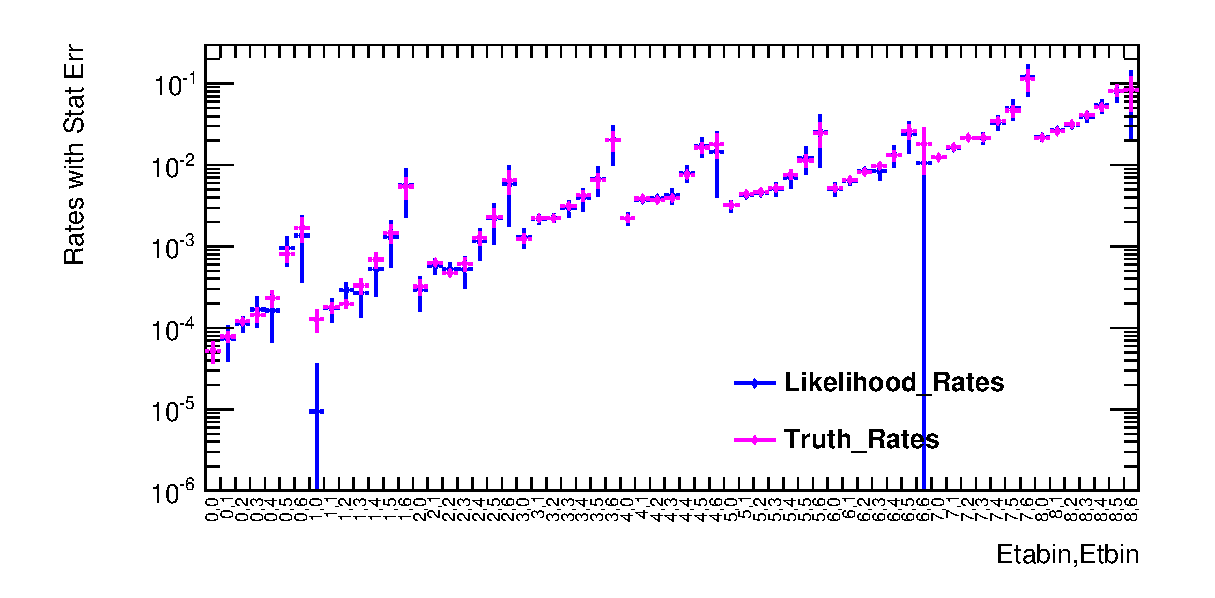
\includegraphics[width=0.8\textwidth]{figures/ChargeMisID/LL_TR_Com.eps}
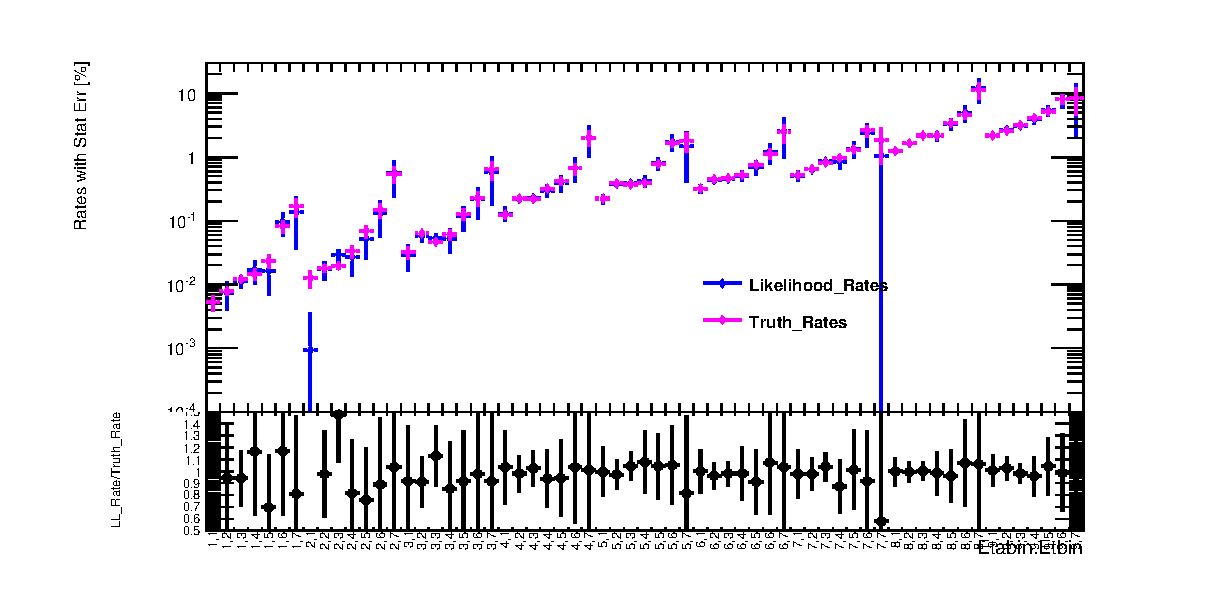
\includegraphics[width=0.8\textwidth]{figures/ChargeMisID/LL_TR_Com_new.eps}

\caption{Comparisons of the charge misID rates obtained with the likelihood method and the truth method. The two sets of rates shown here were both measured with the same \Zee\ MC sample.
Statistical errors are shown. The $x$ axis label is
  the $|\eta|$, \pt\ bin index, as defined in Table~\ref{tab:Etbin and Etabin of mis-charge rate}.}
  
% This is mis-charge rate comparison between likelihood and
%   truth method considering statistic errors. The two sets of rates
%   here are both measured with \Zee\ MC samples. The $x$ axis label is
%   the \eta, \pt\ bin index.}
\label{fig:LL_Truth_Comparison}
\end{figure}  

% Through the comparison, one can see that the rates measured with the
% likelihood method are compatible with that obtained with the truth
% method. The difference between these two sets of rates is taken into account as a systematic in the final measurement.
%

 % \subsubsection{Estimation of the charge misID rates in the data}


The misID rates measured in data using the likelihood method are shown in Figure~\ref{fig:LL_Rates_Egamma}.

% The likelihood method is then applied in the data to measure the charge misID rates.
%  % using the skimmed data from Egamma stream.
% % in Egamma stream we measure the data-driven rates with
% % (\texttt{user.along528.data12\_8TeV.period*.physics\_EGamma.PhysCont.NTUP\_SMWWW.SMN2N\_2\\Lep\_v1\_EXT0}
% % where * is A,B,C,D,E,G,H,I,J,L. These samples are slimmed with loose
% % di-lepton requirement, the di-lepton slim require there are at least 2
% % tagged high \pt\ leptons where tagged high \pt\ means Electron/Muon
% % satisfies any object quality requirement (loose, medium or tight for
% % muons and loose++,\\medium++,tight++,
% % veryLooseLL,looseLL,mediumLL,tightLL, or veryTightLL for electrons)
% % and has a pt of at least 10 GeV.).
%
% They are measured using the same selection described above. This estimation is used as the central value for the charge misID rates measurement. Figure~\ref{fig:LL_Rates_Egamma}, show the central value of the rate and their statistical error as a function of the $|\eta|$ and \pt\ bin index defined in Table~\ref{tab:Etbin and Etabin of mis-charge rate}.

% They are shown as a function of the \eta and \pt\ bin index defined in Table~\ref{tab:Etbin and Etabin of mis-charge rate}, in Figure~\ref{fig:LL_Rates_Egamma}.


\begin{figure}[htp]
\centering
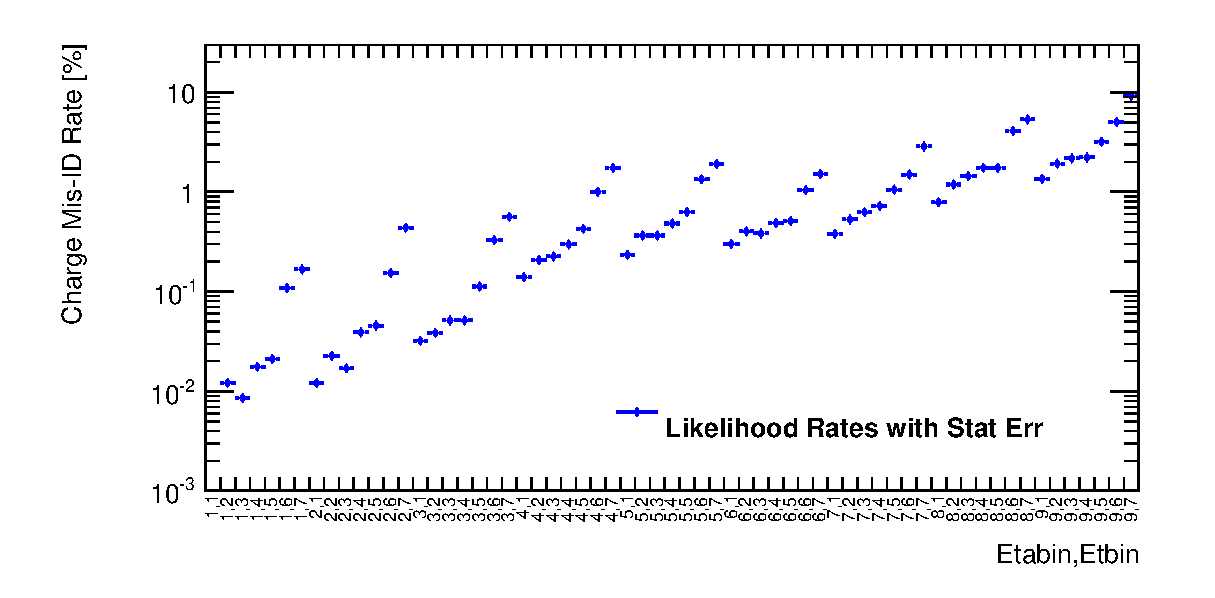
\includegraphics[width=0.8\textwidth]{figures/ChargeMisID/Egamma_LLB_new.eps}
\caption{Electron charge misID rates obtained from data with the likelihood method. Statistical errors are shown. The $x$ axis label is
  the $|\eta|$, \pt\ bin index, as defined in Table~\ref{tab:Etbin and Etabin of mis-charge rate}.}

% This is electron mis-charge rates measured from data with likelihood method and its statistic errors. Label on x axis is \eta, \pt\ bin indices.}
\label{fig:LL_Rates_Egamma}
\end{figure}


 \subsubsection{Systematic effect on charge misID rates due to background contamination}

The contamination of non-$Z\rightarrow{}ee$ processes in the previous selection is taken into account as a systematic.

In order to study this effect, a template fit approach is used. The signal template is obtained from the same MC simulation sample used above, while the background template is obtained from a looser data selection enriched in background events. Due to statistic constraints the background template is obtained in each $|\eta|$ bins, but the $\pt$ bins are grouped together. The event selection for the background template request the presence of a good isolated electron as defined in Section~\ref{sec:Object_selection}, and a second electron failing the tight++ identification cut. 

The two templates are then used on the invariant mass distribution of the electron pairs, in each $\pt$ and $|\eta|$ bins to determine the background contribution, subtract it and recompute the rate by maximizing the likelihood defined in Eq.~(\ref{eq:lnL_chargeMisID}). The difference between this new set of rates and the central value is then taken as a systematic uncertainty on the method, and are summarized in Table~\ref{tab:Charge_MisID_Bkg_Sys}. Further details on this method are also provided in Appendix~\ref{sec:appendix_chargeMisID}.

% The uncertainty due to the background contamination is summarized in Table~\ref{tab:Bkg Sys}.

% We estimate the background effect with
% coarser binning and include the shift in mischarge rate in the
% systematics.


%  We apply the likelihood method and event selection mentioned before
%  to data and we get the data-driven electron mis-charge rates, but
%  the rates are measured from data so there will be background events
%  remaining in the selected events. We use those rates directly
%  measured from data as central values and then subtract the
%  background contribution in the rates, we can calculate another set
%  of likelihood rates using the events without background, we may
%  call those rates clean rates. The difference between central values
%  and clean rates is the background systematic.



\begin{table}
\footnotesize
\centering
\begin{tabular}{c|c|c|c|c|c|c|c|c|c}
  \hline
  \backslashbox{\pt[\GeV]}{$|$\eta$|$} &[0,0.8] &[0.8,1.15] &[1.15,1.60] &[1.60,1.80] &[1.80,2.0] &[2.0,2.20] &[2.20,2.30] &[2.30,2.40] &[2.40,2.50] \\ 
  \hline
  [15,30] &8.85 &5.63 &5.75 &5.85 &5.79 &5.64 &5.64 &5.68 &5.49 \\
  \hline
  [30,40] &5.73 &5.71 &5.83 &5.97 &5.75 &5.78 &5.72 &5.81 &5.59 \\
  \hline
  [40,50] &5.76 &5.69 &5.71 &5.71 &5.65 &5.71 &5.62 &5.71 &5.62 \\
  \hline
  [50,60] &5.74 &5.55 &5.64 &5.53 &5.61 &5.65 &5.41 &5.49 &5.65 \\
  \hline
  [60,80] &5.77 &5.57 &5.71 &5.99 &5.59 &5.66 &5.35 &5.53 &5.41 \\
  \hline
  [80,120] &5.79 &5.63 &5.73 &5.71 &5.74 &5.77 &5.36 &5.74 &5.89 \\
  \hline
  [120,1000] &5.76 &5.71 &5.54 &5.76 &5.52 &5.61 &5.73 &5.98 &6.14  \\
  \hline
\end{tabular}
\caption{Systematic uncertainties on the central value charge misID rates expressed in percent. These uncertainties were obtained considering the impact of the background contamination in the selection.}
% Numbers here are background systematics over central values
%   in percent.}
\label{tab:Charge_MisID_Bkg_Sys}
\end{table} 
 


\subsubsection{Final rates}

The rates with the final errors used in the analysis are shown in Figure~\ref{fig:ChargeMisID_truthRate_finalFig}. The total systematic uncertainty is obtained doing a quadratic sum of the error obtained comparing the MC likelihood method and the truth method, shown in Table~\ref{tab:MCLLTruthSys}, and the error obtained considering the background contamination in the selection. The rates are also given in Table~\ref{tab:LL_finalRates}.

 \begin{figure}[htp]
 \centering
 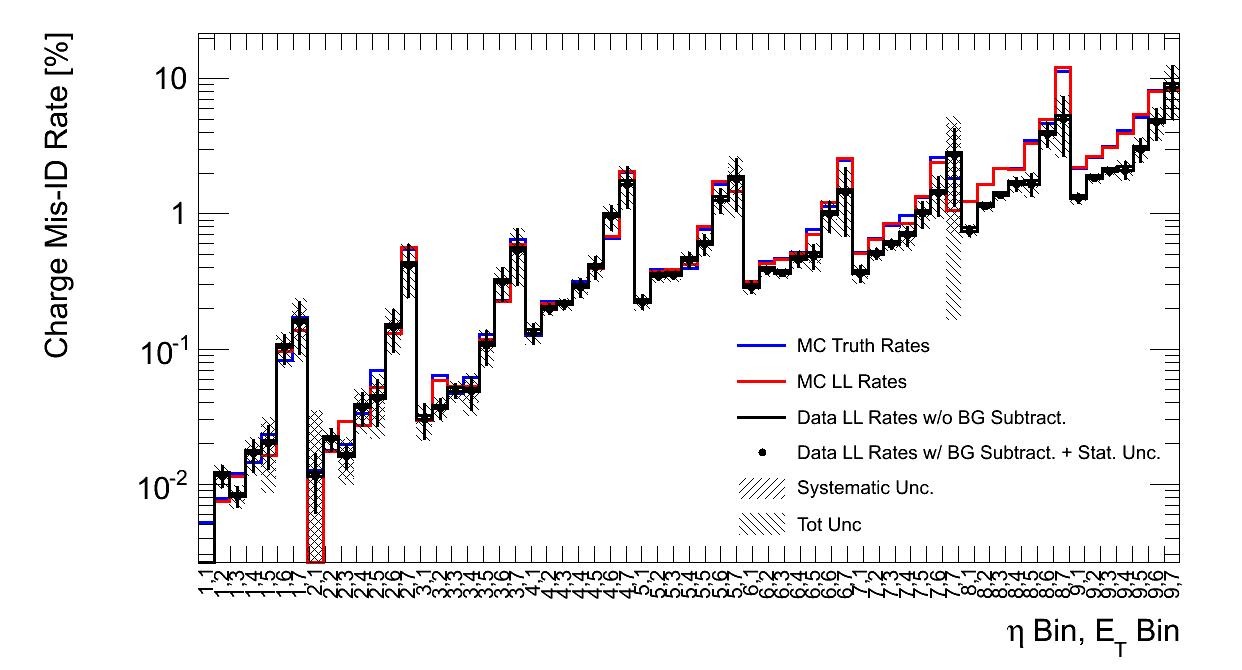
\includegraphics[width=0.8\textwidth]{figures/ChargeMisID/Validation_ChargeMisIDRates_PTvsEta_FinalRateWithSys.png}
 \caption{Electron charge misID rates obtained from data with the likelihood method. All the errors are now shown. The $x$ axis label is
  the $|\eta|$, \pt\ bin index, as defined in Table~\ref{tab:Etbin and Etabin of mis-charge rate}.}
 \label{fig:ChargeMisID_truthRate_finalFig}
 \end{figure}

\begin{table}
\footnotesize
\centering
\begin{tabular}{c|c|c|c|c|c|c|c|c|c}
  \hline
  \backslashbox{\pt[\GeV]}{$|$\eta$|$} &[0,0.8] &[0.8,1.15] &[1.15,1.60] &[1.60,1.80] &[1.80,2.0] &[2.0,2.20] &[2.20,2.30] &[2.30,2.40] &[2.40,2.50] \\
  \hline
  [15,30] & $> 100$ & $> 100$ &9.24 &3.12 &0.70 &0.05 &2.27 &0.25 &0.80 \\
  \hline
  [30,40] & 5.98 &2.58 &9.91 &2.14 &2.97 &3.84 &2.51 &0.63 &2.44\\
  \hline
  [40,50] & 6.22 &32.26 &11.36 &2.19 &4.12 &2.17 &3.52 &0.43 &2.13 \\
  \hline
  [50,60] & 14.22 &22.92 &17.20 &6.72 &7.13 &2.08 &14.80 &1.75 &4.52 \\
  \hline
  [60,80] & 43.45 &32.03 &9.39 &6.14 &3.93 &9.86 &1.19 &4.22 &3.84 \\
  \hline
  [80,120] & 14.59 &12.57 &2.51 &3.14 &4.73 &6.90 &9.40 &6.40 &1.34 \\
  \hline
  [120,1000] & 23.46 &3.02 &9.53 &1.02 &22.98 &3.17 &73.12 &5.61 &3.31 \\
  \hline
\end{tabular}
\caption{The absolute value of the difference between the charge mis-identification rates derived in MC using the truth method and using the likelihood method.  Numbers
are shown as a percent of the MC likelihood method.  These are transported to the likelihood rates in data and used as a systematic. }
\label{tab:MCLLTruthSys}
\end{table}



\begin{table}
\footnotesize
\centering
\begin{tabular}{c|c|c|c|c|c|c|c|c|c}
  \hline
  \backslashbox{\pt[\GeV]}{$|$\eta$|$} &[0,0.8] &[0.8,1.15] &[1.15,1.60] &[1.60,1.80] &[1.80,2.0] &[2.0,2.20] &[2.20,2.30] &[2.30,2.40] &[2.40,2.50] \\
  \hline
  $ \times 10^{}$
  [15,30] &$1.7370\times 10^{-11}$ &$9.4036\times 10^{-6}$ &0.0003 &0.0013 &0.0022 &0.0032 &0.0051 &0.0124 &0.0219\\
  \hline
  [30,40] &$7.4276\times 10^{-5}$ &0.0002 &0.0006 &0.0022 &0.0038 &0.0043 &0.0064 &0.0165 &0.0268 \\
  \hline
  [40,50] &0.0001 &0.0003 &0.0005 &0.0023 &0.0039 &0.0046 &0.0085 &0.0218 &0.0311 \\
  \hline
  [50,60] &0.0002 &0.0003 &0.0005 &0.0030 &0.0042 &0.0051 &0.0085 &0.0213 &0.0394 \\
  \hline
  [60,80] &0.0002 &0.0005 &0.0012 &0.0040 &0.0080 &0.0070 &0.0134 &0.0332 &0.0540 \\
  \hline
  [80,120] &0.0009 &0.0013 &0.0023 &0.0068 &0.0172 &0.0122 &0.0239 &0.0497 &0.0810 \\
  \hline
  [120,1000] &0.0014 &0.0056 &0.0059 &0.0204 &0.0147 &0.0255 &0.0106 &0.1208 &0.0820  \\
  \hline
\end{tabular}
\caption{Electron charge mis-ID rates, obtained with the likelihood method on the data.}
\label{tab:LL_finalRates}
\end{table}




Although the likelihood method, which is used to determined the rates from the data, was validated in MC using the truth method, it is quite important to validate the rates as much as possible, and to verify that if there are remaining differences they are covered within the systematic uncertainties that were assigned.

%As already stated, the charge misID rates are particularely important for the determination of the $WZ$ and $ZZ$ background contamination in the 0SFOS region. Therefore two more tests are conducted to test their validity.

We performed a test to recompute the charge misID rates using the truth method and a $WZ$ MC sample, and compare these new rates to the old one obtained with the $Z\to{}ee$ events. In principle, the charge misID is mostly due to detector effects, and it is therefore not expected to see any differences using one physics process or another one, as long as the GEANT4 geometry of the detector that was used to generate the events is the same. To perform this study, given the lower statistic available in the $WZ$ MC sample a different binning is used, it is summarized in Table~\ref{tab:Etbin and Etabin of mis-charge rate for WZ comparisons}. The new rates obtained are compared in Figure~\ref{fig:ChargeMisID_truthRate_Zee_WZ}. In this figure only the statistical error of each measurement is shown. A very good agreement between the two sets of rates is observed.



\begin{table}[htp]
\centering

\begin{tabular}{c|c||c|c}
	 \hline
	  $|\eta|$ bins & $|\eta|$ bin index   & \pt\ bins [\GeV] & \pt\ bin index \\
 	 \hline
	  $[0, 1.15]   $   & 0 	   &  $[15, 40]$ & 0 \\
	  $[1.15, 1.8] $   & 1 	   &  $[40, 60]$ & 1 \\
	  $[1.8, 2.2] $   & 2	   &  $[60, 100]$ & 2 \\
	  $[2.2, 2.5] $   & 3 	   &  $[100, 1000]$ & 3 \\

  \hline
\end{tabular}
\caption{The $|\eta|$ and \pt\ bins used for the comparison of mischarge
  rate obtained with MC $Z\to{}ee$ sample and MC $WZ$ sample. The bin index used in the 1D figures~\ref{fig:ChargeMisID_truthRate_Zee_WZ} are given.}
\label{tab:Etbin and Etabin of mis-charge rate for WZ comparisons}
\end{table}



 \begin{figure}[htp]
 \centering
 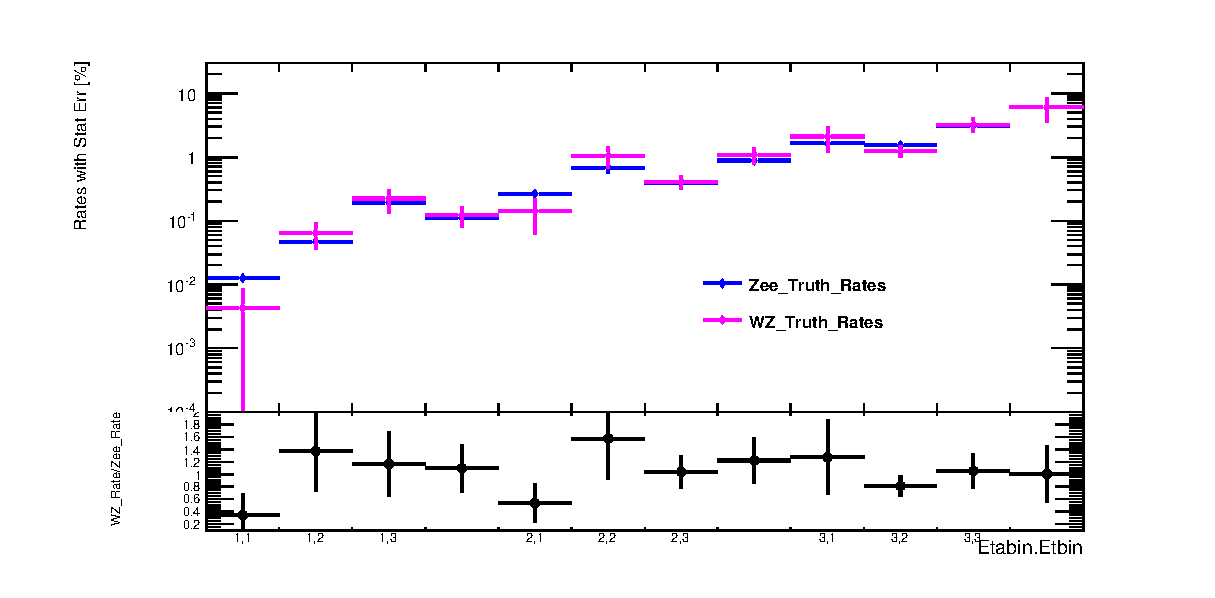
\includegraphics[width=0.8\textwidth]{figures/ChargeMisID/Validation_ChargeMisIDRates_PTvsEta_CompareSSRate.eps}
 \caption{Electron charge misID rates obtained from MC $Z\to{}ee$ with the likelihood method are compared with rates obtained using the truth method in a MC $WZ$ sample. Errors shown here are purely statistics. The $x$ axis label is
  the $|\eta|$, \pt\ bin index, as defined in Table~\ref{tab:Etbin and Etabin of mis-charge rate for WZ comparisons}.}
 \label{fig:ChargeMisID_truthRate_Zee_WZ}
 \end{figure}


\subsubsection{Application and validation of rates}
As already stated, the charge misID rates are primarily important for the determination of the $WZ$ and $ZZ$ background contamination in the 0SFOS region. 
Once derived, the rates are applied to $WZ$ and $ZZ$ MC samples based on whether or not a charge flip could cause the event to appear in the 0 SFOS region.  
In particular, the following di-boson decays are considered:
\begin{itemize}
\item $WZ\rightarrow e^{\pm}\nu~ e^{+}e^{-}$
\item $WZ\rightarrow \mu^{\pm}\nu~ e^{+}e^{-}$
\item $WZ\rightarrow \tau^{\pm}\nu~ e^{+}e^{-}$
\item $ZZ\rightarrow e^{+}e^{-}~e^{+}e^{-}$
\item $ZZ\rightarrow \mu^{+}\mu^{-}~ e^{+}e^{-}$
\end{itemize}
No other decay channels are considered.  These all share in common that they have at least one electron-positron pair.  
Except for the $WZ\rightarrow \tau^{\pm}\nu~e^{+}e^{-}$ decay channel, decay channels with tau leptons are not considered
because they are suppressed by the tau branching fraction and are considered to be negligible.

The charge mis-identification rates are then applied to these channels on an event-by-event basis as follows.
For each event that is processed, its decay channel is identified at truth level. Each reconstructed lepton
is examined  and assigned a rate, or a probability to charge flip, based on its reconstructed $\pt$ and $\eta$ values.
The probability for a charge flip to occur in an event is then approximately the sum of rates for the individual electrons:
\begin{equation}
\textrm{Probability of Charge Mis-Identification in Event} = \sum_{i \in \textrm{Electrons}}  \textrm{Rate}(\pt^i,\eta^i) + \textrm{Higher Order Terms}
\end{equation}
Higher order terms where multiple electrons are charge mis-identified is small and considered to be negligible.
We are only concerned with the probability that a charge flip results in the event falling into the 0 SFOS region. 
Consider a step function, $\Theta(e)$, defined for an individual event:
\[
\Theta(e) = 
\begin{cases}
\hfill 1 \hfill & \text{if flipping charge of $e$ classifies event as 0 SFOS} \\
\hfill 0 \hfill & \text{if flipping charge of $e$ does NOT classify event as 0 SFOS}\\
\end{cases}
\]
Then the probability that a charge mis-identification occurs and results in the event falling in the 0 SFOS region is:
\begin{equation}
\textrm{Probability that event is classified as 0 SFOS} = \sum_{i \in \textrm{Electrons}}  \textrm{Rate}(\pt^i,\eta^i)\Theta(i) + \textrm{Higher Order Terms}
\end{equation}
Again, we ignore the case where multiple electrons have their charge mis-identified.  
This probability is then used as an event by event weight. 



Once the weight has been determined, we then artificially flip the charge of one of the electrons/positrons in the event.
If there is only one electron in the event that will lead the event to fall in the 0 SFOS region, its charge is flipped
and one proceeds to the next event.  However, if there are multiple electrons in the event, there is an ambiguity that must be resolved
about which electron's charge should be flipped. One must then be careful in this case to not introduce any bias.
We decided to choose a procedure where we pick a single electron from the event at random based on the charge flip rates
of the individual electrons. Thus, for an individual electron in an event, the probability that it is chosen to have its charge
flipped is:
\begin{equation}
\textrm{Probability that $e$ has charge flipped} = \textrm{Rate}(\pt^e,\eta^e)\Theta(e)~/\sum_{i \in \textrm{Electrons}} \textrm{Rate}(\pt^i,\eta^i)\Theta(i)
\end{equation}

Consider an example 
where the event under consideration comes from the decay $WZ\rightarrow e^{+}\nu e^{+}e^{-}$. Assume all three charged leptons pass reconstruction and are selected then label them as: $e^{+}_1~e^{+}_2e^{-}_3$. In this case,
the only way that this event could be classified as 0 SFOS when flipping the charge of only one electron/positron is to flip the charge of the electron.
Thus, $\Theta(e^{+}_1)=\Theta(e^{+}_2)=0$ and $\Theta(e^{-}_3)=1$.  The event weight will then be equal to the rate of charge mis-identification for  $e^{-}_3$ and it
will have it's charge flipped to be positive.

Now consider an example of an event with the decay of $ZZ\rightarrow \mu^{+}\mu^{-}~ e^{+}e^{-}$.
If all four leptons are reconstructed and selected, the event will not be considered at all in the three lepton selection of this analysis, so consider the 
case where the $\mu^{+}$ is not selected leaving three leptons labeled as: $\mu^{-}_1 e^{+}_2 e^{-}_3$.  The probability for the muon to charge flip
is negligible which leaves the electron and the positron. Flipping the charge of either one at a time will result in the event being classified as 0 SFOS.  Thus, in
this case $\Theta(\mu^{-}_1)=0$ and $\Theta(e^{+}_2)=\Theta(e^{-}_3)=1$. The event weight will then be the sum of the rates for $e^{+}_2$ and $e^{-}_3$.
The probability that the electron has its charge flipped is then $\frac{\textrm{Rate}(e^{-}_3) }{ \textrm{Rate}(e^{+}_2)+ \textrm{Rate}(e^{-}_3)}$ and similarly for the positron.

This procedure has been validated on the $WZ$ and $ZZ$ samples by comparing the predictions taken directly from MC to the predictions reweighted in the 0 SFOS signal region using the procedure just described. This is done in Figure~\ref{fig:ChargeMisID_Validation_WZ} for the $WZ$ samples and on Figure~\ref{fig:ChargeMisID_Validation_ZZ} for the $ZZ$ samples. It can be seen the agreement in the shape looks good for all the distributions. An offset between the two distributions is observed. This difference is covered partially by the systematic uncertainties of the method.  Any remaining difference could be expected from the difference in rates observed at high $\eta$ and high $E_{T}$ as seen in Fig.~\ref{fig:ChargeMisID_truthRate_finalFig} and serves as justification for using the data-driven method.

There is no special treamtent of the charge mis-identification contribution to other background contributions in the 0 SFOS region or to any contributions to the 
1 and 2 SFOS signal regions, including diboson processes, as the effect is expected to be very small.  Any charge mis-identification events are thus taken directly 
from MC in this case.


 \begin{figure}[htp]
 \centering
 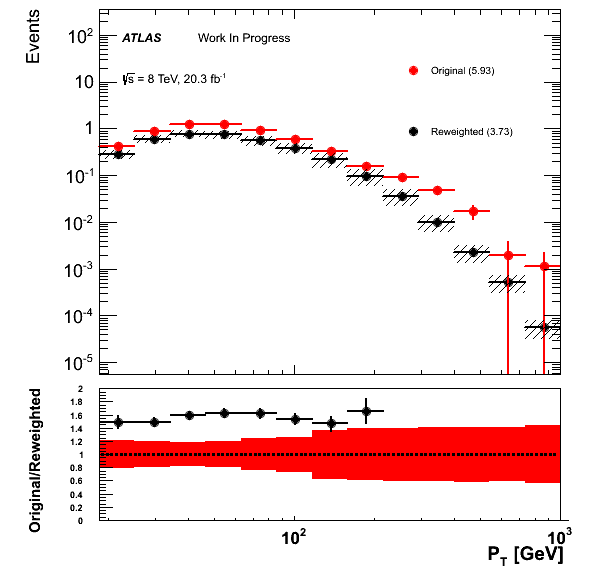
\includegraphics[width=0.4\textwidth]{figures/ChargeMisID/Validation_ChargeMisIDRates_WZ_PTLepton.png}
 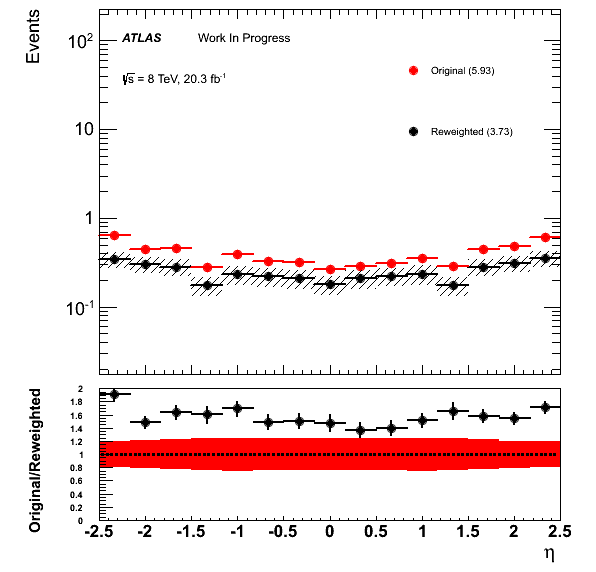
\includegraphics[width=0.4\textwidth]{figures/ChargeMisID/Validation_ChargeMisIDRates_WZ_EtaLepton.png}
 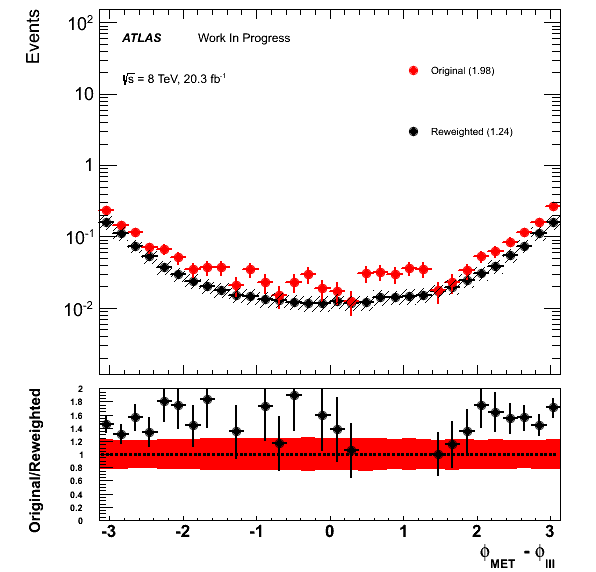
\includegraphics[width=0.4\textwidth]{figures/ChargeMisID/Validation_ChargeMisIDRates_WZ_DeltaPhi.png}
 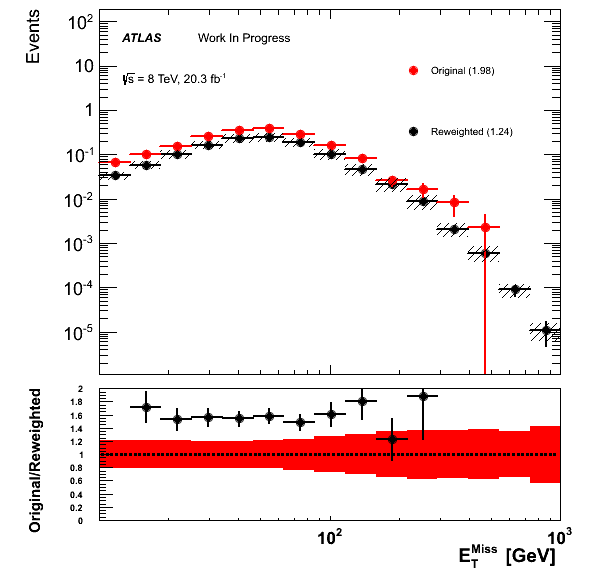
\includegraphics[width=0.4\textwidth]{figures/ChargeMisID/Validation_ChargeMisIDRates_WZ_MET.png}
 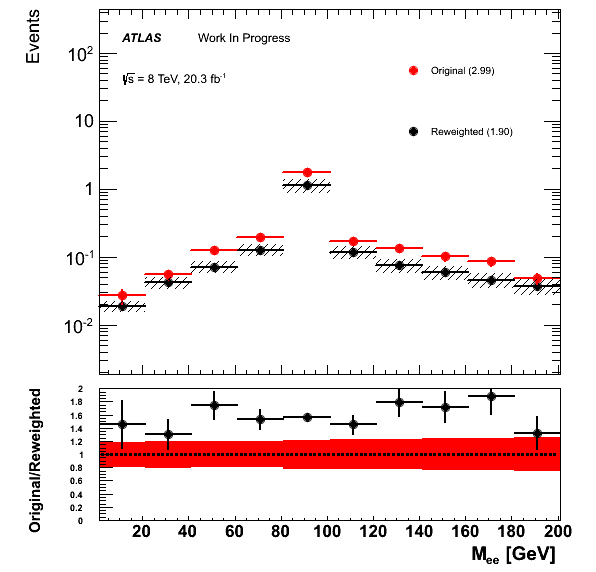
\includegraphics[width=0.4\textwidth]{figures/ChargeMisID/Validation_ChargeMisIDRates_WZ_Mee.png}
 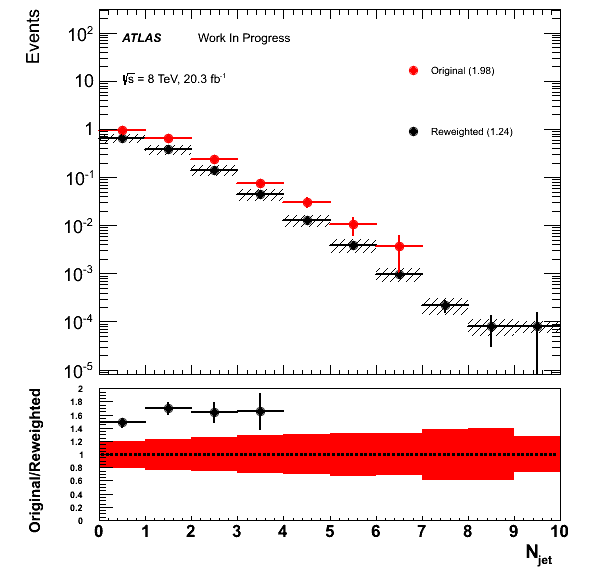
\includegraphics[width=0.4\textwidth]{figures/ChargeMisID/Validation_ChargeMisIDRates_WZ_JetMultiplicity.png}

 \caption{Validation of the charge mis-ID rates comparing MC $WZ\rightarrow \ell ee$ ($\ell=e,\mu$) samples reweighted with the charge misID rates measured in the MC $Z\to{}ee$ 
 sample to the original MC predictions. Distribution of lepton $p_{T}$, $\eta$, $\Delta \phi(3l,E_{T}^{Miss})$,\met{}, Same-sign di-electron invariant mass, and jet multiplicity.}
 \label{fig:ChargeMisID_Validation_WZ}
 \end{figure}
 
 
 \begin{figure}[htp]
 \centering
 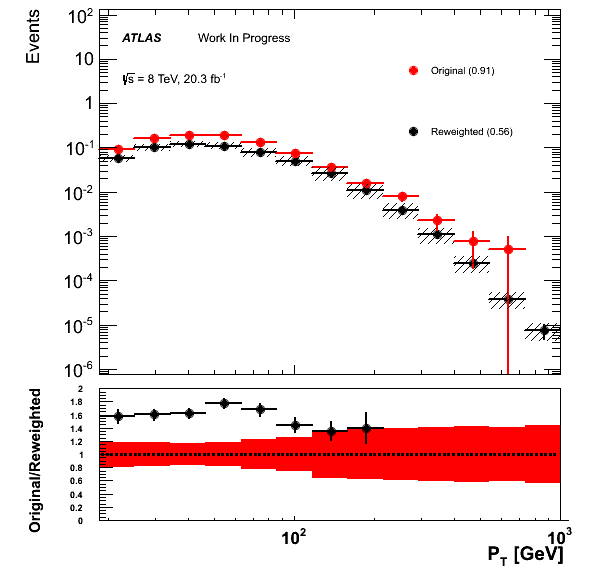
\includegraphics[width=0.4\textwidth]{figures/ChargeMisID/Validation_ChargeMisIDRates_ZZ_PTLepton.png}
 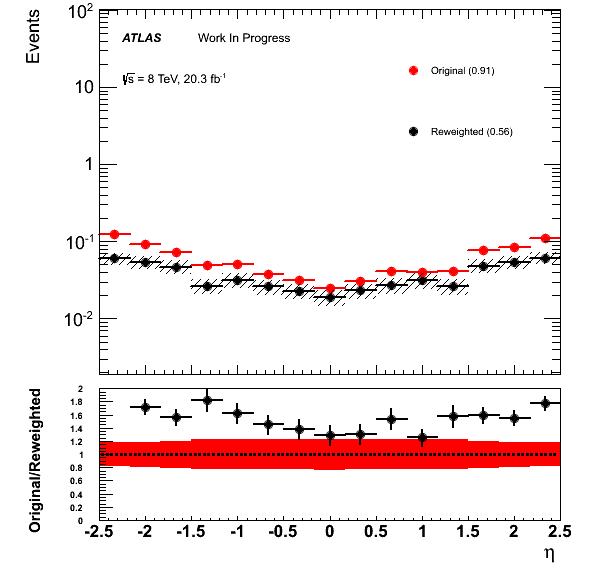
\includegraphics[width=0.4\textwidth]{figures/ChargeMisID/Validation_ChargeMisIDRates_ZZ_EtaLepton.png}
 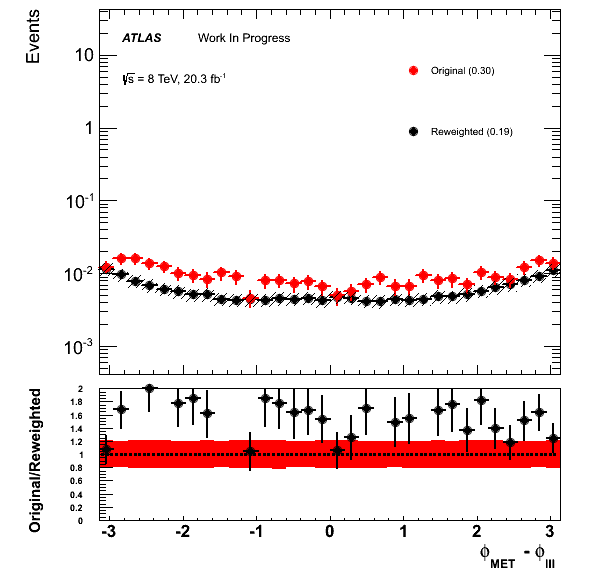
\includegraphics[width=0.4\textwidth]{figures/ChargeMisID/Validation_ChargeMisIDRates_ZZ_DeltaPhi.png}
 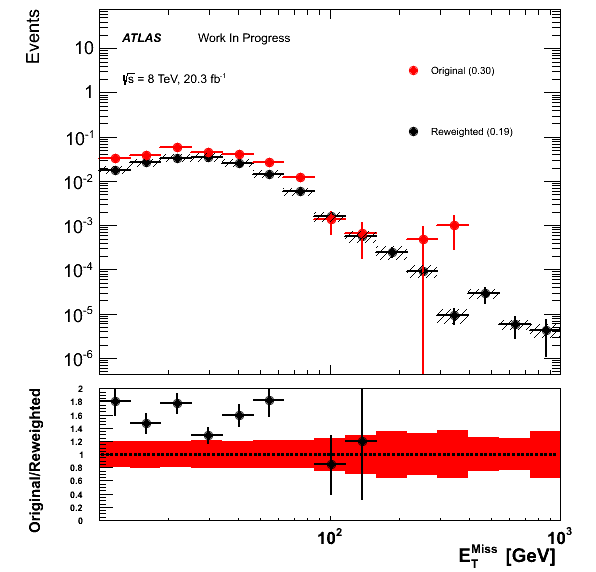
\includegraphics[width=0.4\textwidth]{figures/ChargeMisID/Validation_ChargeMisIDRates_ZZ_MET.png}
 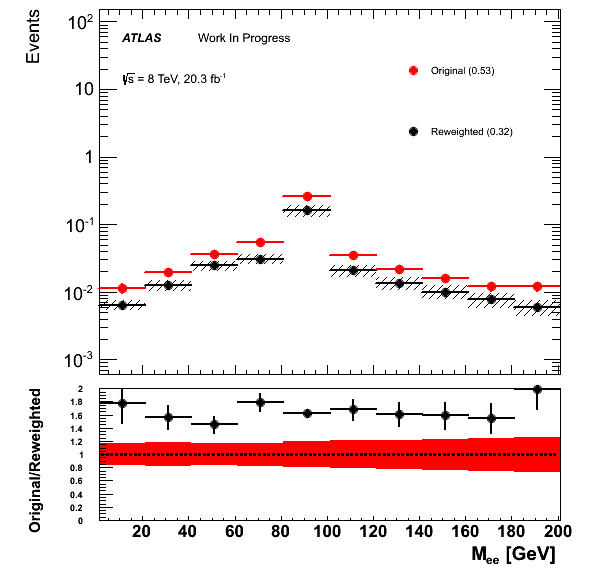
\includegraphics[width=0.4\textwidth]{figures/ChargeMisID/Validation_ChargeMisIDRates_ZZ_Mee.png}
 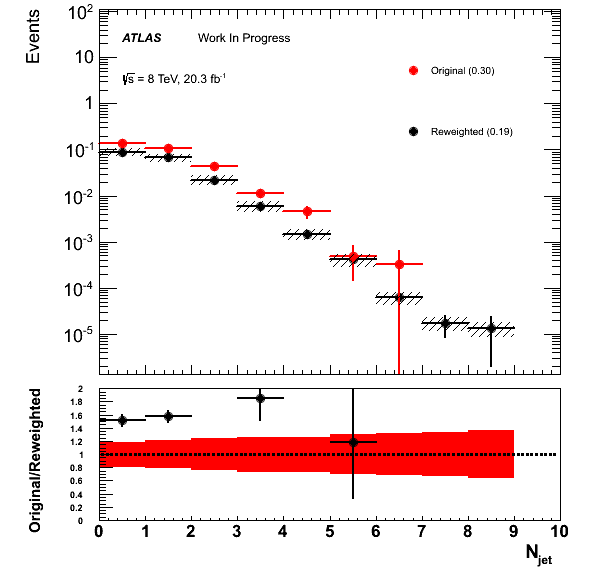
\includegraphics[width=0.4\textwidth]{figures/ChargeMisID/Validation_ChargeMisIDRates_ZZ_JetMultiplicity.png}

 \caption{Validation of the charge mis-ID rates comparing MC $ZZ\rightarrow \ell \ell ee$ ($\ell=e,\mu$) samples reweighted with the charge misID rates measured in the MC $Z\to{}ee$ 
 sample to the original MC predictions. Distribution of lepton $p_{T}$, $\eta$, $\Delta \phi(3l,E_{T}^{Miss})$,\met{}, Same-sign di-electron invariant mass, and jet multiplicity.}
 \label{fig:ChargeMisID_Validation_ZZ}
 \end{figure}







\subsubsection{Background samples}
\label{sec:www_bg}

There are other processes produced in proton-proton collisions at the LHC
which can mimic the signal processes. These are referred to as background processes.
In many cases, the background processes are either
more abundant than or of a similar abundance to
the signal. As a result, they must be well understood if there is any hope
of distinguishing between the two. The background processes to the signal
are characterized by having either at least three prompt leptons, meaning they
come directly from the hard scattering process;  
two prompt leptons and an isolated photon, which can mimic an electron;
or two prompt leptons and a jet that mimics a lepton.
The first two are estimated primarily using MC simulation while the third type
is estimated using the data itself. 
This will be described in more detail in \sec\ref{sec:bg_fake}.
For now, we will focus only on the processes estimated using MC simulation.

The most important backgrounds are those with at least three prompt leptons, 
hereby referred to as the prompt backgrounds. Of these prompt backgrounds,
the $WZ$ process is the most important since it has a 
large cross-section (compared to the signal)
and results in a final state with exactly three leptons. Another important 
prompt background is the $ZZ$ process,
which has a similar cross-section to the $WZ$ process, but is typically 
selected by producing
four leptons and then not measuring one. Thus, this process is supressed by the 
efficiency for not measuring the presence of a lepton. 
These are collectively referred to as the di-boson processes, sometimes
indicated as $VV$ where $V=W/Z$ (the $WW$ process is also considered
but can only produce at most two prompt leptons making it negligible). 
The di-boson processes are produced using the 
the \powheg~\cite{Alioli:2008gx,Nason:2004rx,Frixione:2007vw,Alioli:2010xd} generator
with the CT10 NLO PDF set and 
hadronized through \pythiaeight~using the AU2 tune, same as the signal.

Other prompt backgrounds 
inlcude tri-boson processes like $ZWW$ and $ZZZ$ 
(typically referred to collectively as $VVV$)
and \ttV~production. Tri-boson processes
have cross-sections of a similar size to the signal but are supressed 
for a similar reason
as the $ZZ$, since these can produce either four or six lepton final 
states. 
\ttV~production is when a vector
boson is produced in conjuction with a \tt~pair. 
Since the top quark almost always decays
into a $W$-boson and a $b$-quark, \ttV~production also results in an intermediate
state of three vector bosons which ultimately results in a three to four lepton
final state.
The $VVV$ and \ttV~processes were generated using \madgraph with the 
CTEQ6L1 PDF set and hadronized
using \pythiasix~\cite{PYTHIA} with the AUET2B~\cite{ATL-PHYS-PUB-2011-009} 
tune.

The second category of backgrounds to consider are those with two 
prompt leptons and a photon. We will call these the photon backgrounds.
This background occurs entirely from the di-boson process $Z\gamma$
where the $Z$ boson decays to two leptons and the photon mimics an electron.
A photon is measured
by observing an energy deposit in the electromagnetic calorimeter 
without any associated track in the inner detector.
A photon can mimic an electron
if it converts into an electron-positron
pair while still inside the inner detector, thereby leaving a track 
in the inner detector while still leaving an energy deposit in the 
calorimeter, the tell-tale sign of an electron.
The $Z\gamma$ samples were generated with the \sherpa~\cite{sherpa} generator 
and the CT10 PDF set.  %hadronization? CT10 NLO? Or LO?
In addition to this process, the $W\gamma$ process behaves similarly 
but only has one prompt lepton in addition to the photon, so it is negligible.
Still, we generate it by using
the \alpgen~\cite{ALPGEN} generator with the CTEQ6L1 PDF set
and hadronize it using \jimmy~\cite{Jimmy} with the AUET2C~\cite{ATL-PHYS-PUB-2011-009} 
tune.

Some of the di-boson and tri-boson processes just discussed can also be produced
through loop induced processes or double parton scattering.
The $WW$ and $ZZ$
loop induced processes are generated using the gg2ZZ~\cite{Binoth:2008pr} 
and gg2WW~\cite{Binoth:2006mf} generators with the CT10 PDF set and
hadronized using JIMMY with the AU2 tunes.
The double parton scattering
processes are generated using \pythiaeight with the AU2 
tunes and the CTEQ6L1 PDF set. 

The last category of backgrounds are those with prompt leptons plus
jets that mimic leptons. These are nominally estimated using the data
as decribed in \sec\ref{sec:bg_fake}. However, some of the contributions
to this background can be simulated using MC as a cross-check of 
the estimate from data and for other studies. The main contributions
to this are the single boson processes ($V+$jets) and \tt~production.
These are processes with very large cross-sections so
that even though the probability for a jet mimicking a lepton is small,
the size of the cross-section means that their contribution is non-negligible.
The single boson process of $Z+$jets are generated using \sherpa~ with the CT10
PDF set while the $W+$jets processes are generated using \alpgen~ with
the CTEQ6L1 PDF set and hadronized using \jimmy~with the AUET2C tunes.
For the $Z+$jets samples, special care must be taken to remove any overlap 
between with the $Z\gamma$ simulated samples described earlier.
Meanwhile, the \tt~processes are generated using the \mcatnlo~\cite{MCatNLO}
generator with the CT10 PDF set and hadronized in JIMMY.  %what is the tune?
Finally, this background also has contributions from single top production,
though it is less important. Single top production is simulated separately 
for the s-channel, t-channel, and $Wt$-channel. The s-channel 
and $Wt$-channel are generated using \mcatnlo~with the CT10 PDF set and 
hadronized through \jimmy~ while the t-channel is generated using \madgraph~
with the CTEQ6L1 PDF set and hadronized using \pythiasix~with the AUET2B tunes.


\section{Corrections and Systematic Uncertainties}
\label{sec:systematics}

The predictions for the signal and background are subject
to the choices made in building the model described thus
far in \sec\ref{sec:www}. If we are to believe our predictions
we must understand how sensitive the predictions are to these choices.
To that end, we also compute the prediction for numerous variations
on the nominal prediction. 
Each one of these variations is called a systematic uncertainty. 
Each systematic uncertainty is designed to assess the sensitivity
to a given choice made when building the model. 
This analysis has almost 50 different systematic
uncertainties, each of which is varied independently. The size of 
each systematic uncertainty
is treated as a separate nuisance parameter
as input to the statistical model used in the interpretation of the model
when compared to data, described later in \sec\ref{sec:measurement}.

The systematic uncertainties can be split up into four categories:
theory, methodology, experiment, and luminosity. 
I will summarize them below, in each case giving the 
size of the uncertainties in the three signal regions. 
Some of these variations have 
been mentioned already in previous sections but will be
referred to here again for completeness.

\subsection{Theoretical Uncertainties}




\begin{table}[ht]
\centering
\small\renewcommand{\tabcolsep}{4pt}
\begin{tabular}{|cl||ccccccc|c||c|}
\hline
 & & \multicolumn{8}{c||}{Background} & Signal \\ 
 & & $WZ$ & $ZZ$ & $VVV$ & $t\overline{t}+V$ & DPS & $Z\gamma$ & Fake & Total & \\ 
 & & &  &  &  &  &  & (Data) & BG & \\ 
\hline\hline
\multirow{2}{*}{Signal}
&PDF & --- & --- & --- & --- & --- & --- & --- & --- &  $2.80$ \\ 
\cline{2-11}
& $\mu_{R}$ and $\mu_{F}$ Choice &  --- &  --- &  --- &  --- &  --- &  --- &  --- &  --- & $2.60$\\ 
\hline
\multirow{5}{*}{Norm.}
& $WZ$ & $10.00$&  --- &  --- &  --- &  --- &  --- &  --- & $2.63$&  ---\\ 
\cline{2-11}
& $ZZ$ &  --- & $15.00$&  --- &  --- &  --- &  --- &  --- & $0.42$&  ---\\ 
\cline{2-11}
& $VVV$ &  --- &  --- & $30.00$&  --- &  --- &  --- &  --- & $1.44$&  ---\\ 
\cline{2-11}
& $t\overline{t}+V$ &  --- &  --- &  --- & $30.00$&  --- &  --- &  --- & $0.50$&  ---\\ 
\cline{2-11}
& DPS &  --- &  --- &  --- &  --- & $50.00$&  --- &  --- &  --- &  ---\\ 
\hline
\end{tabular}

\caption{Size of theoretical uncertainties in percent for the 0 SFOS signal region. The background uncertainties are shown for the individual background components as well as the total. The signal uncertainty is shown separately. Those marked --- are either not applicable or below 0.02 \% and thus considered to be negligible}
\label{tab:sys_theory_0sfos}
\end{table}

\begin{table}[ht]
\centering
\small\renewcommand{\tabcolsep}{4pt}
\begin{tabular}{|cl||ccccccc|c||c|}
\hline
 & & \multicolumn{8}{c||}{Background} & Signal \\ 
 & & $WZ$ & $ZZ$ & $VVV$ & $t\overline{t}+V$ & DPS & $Z\gamma$ & Fake & Total & \\ 
 & & &  &  &  &  &  & (Data) & BG & \\ 
\hline\hline
\multirow{2}{*}{Signal}
& PDF &  --- &  --- &  --- &  --- &  --- &  --- &  --- &  --- & $2.80$\\ 
\cline{2-11}
& $\mu_{R}$ and $\mu_{F}$ Choice &  --- &  --- &  --- &  --- &  --- &  --- &  --- &  --- & $2.60$\\ 
\hline
\multirow{5}{*}{Norm.}
& $WZ$ & $10.00$&  --- &  --- &  --- &  --- &  --- &  --- & $8.05$&  ---\\ 
\cline{2-11}
& $ZZ$ &  --- & $15.00$&  --- &  --- &  --- &  --- &  --- & $0.59$&  ---\\ 
\cline{2-11}
& $VVV$ &  --- &  --- & $30.00$&  --- &  --- &  --- &  --- & $0.28$&  ---\\ 
\cline{2-11}
& $t\overline{t}+V$ &  --- &  --- &  --- & $30.00$&  --- &  --- &  --- & $0.10$&  ---\\ 
\cline{2-11}
& DPS &  --- &  --- &  --- &  --- & $50.00$&  --- &  --- &  --- &  ---\\ 
\hline
\end{tabular}

\caption{Size of theoretical uncertainties in percent for the 1 SFOS signal region. The background uncertainties are shown for the individual background components as well as the total. The signal uncertainty is shown separately. Those marked --- are either not applicable or below 0.02 \% and thus considered to be negligible}
\label{tab:sys_theory_1sfos}
\end{table}

\begin{table}[ht]
\centering
\small\renewcommand{\tabcolsep}{4pt}
\begin{tabular}{|cl||ccccccc|c||c|}
\hline
 & & \multicolumn{8}{c||}{Background} & Signal \\ 
 & & $WZ$ & $ZZ$ & $VVV$ & $t\overline{t}+V$ & DPS & $Z\gamma$ & Fake & Total & \\ 
 & & &  &  &  &  &  & (Data) & BG & \\ 
\hline\hline
\multirow{2}{*}{Signal}
& PDF &  --- &  --- &  --- &  --- &  --- &  --- &  --- &  --- & $2.80$\\ 
\cline{2-11}
& $\mu_{R}$ and $\mu_{F}$ Choice &  --- &  --- &  --- &  --- &  --- &  --- &  --- &  --- & $2.60$\\ 
\hline
\multirow{5}{*}{Norm.}
& $WZ$ & $10.00$&  --- &  --- &  --- &  --- &  --- &  --- & $8.83$&  ---\\ 
\cline{2-11}
& $ZZ$ &  --- & $15.00$&  --- &  --- &  --- &  --- &  --- & $0.70$&  ---\\ 
\cline{2-11}
& $VVV$ &  --- &  --- & $30.00$&  --- &  --- &  --- &  --- & $0.23$&  ---\\ 
\cline{2-11}
& $t\overline{t}+V$ &  --- &  --- &  --- & $30.00$&  --- &  --- &  --- & $0.07$&  ---\\ 
\cline{2-11}
& DPS &  --- &  --- &  --- &  --- & $50.00$&  --- &  --- & $0.11$&  ---\\ 
\hline
\end{tabular}

\caption{Size of theoretical uncertainties in percent for the 2 SFOS signal region. The background uncertainties are shown for the individual background components as well as the total. The signal uncertainty is shown separately. Those marked --- are either not applicable or below 0.02 \% and thus considered to be negligible}
\label{tab:sys_theory_2sfos}
\end{table}

The theoretical uncertainties are those on the signal PDF and 
on the background cross-section predictions.
They are summarized for the 0, 1, and 2 SFOS regions
in \tab\ref{tab:sys_theory_0sfos}, 
\tab\ref{tab:sys_theory_1sfos}, and
\tab\ref{tab:sys_theory_2sfos}, respectively.
The motivation for the PDF uncertainties has been described
already in \sec\ref{sec:pdf}. 
There are several uncertainties evaluated on the signal PDF, all of which
are described in more detail in \sec\ref{sec:signal}. These
are the PDF choice, including uncertainties reported by the individual
PDFs, as well as variations in the renormalization and factorization scales.
The effect on the signal prediction from these is around 2-3\%.

The most important MC backgrounds have uncertainties evaluated on their
cross-section.  In particular, these are the uncertainties on the 
normalization of the $WZ$, $ZZ$, $Z\gamma$, $VVV$, $\ttV$, 
and DPS background predictions
described in \sec\ref{sec:bg_estimates} and summarized in \tab\ref{tab:mcnorm}.
Their impact when propagated to the final background prediction
varies by channel. In general, the uncertainty on the $WZ$ prediction is the 
largest, contributing about 2.6\% in the 0 SFOS region and around 8-9\%
in the 1 and 2 SFOS regions.  In the 0 SFOS region, the uncertainty 
on the $VVV$ prediction contributes about 1.4\% and that on the $ZZ$ prediction
is about 0.4\%; all others fall below that. 
In the 1 and 2 SFOS regions the $ZZ$ uncertainty is around 0.6-0.7\%; the
rest are negligible. 

\subsection{Methodological Uncertainties}

\begin{table}[ht!]
\centering
\small\renewcommand{\tabcolsep}{4pt}
\begin{tabular}{|cl||ccccccc|c||c|}
\hline
 & & \multicolumn{8}{c||}{Background} & Signal\\ 
 & & $WZ$ & $ZZ$ & $VVV$ & $t\overline{t}+V$ & DPS & $Z\gamma$ & Fake & Total & \\ 
 & & &  &  &  &  &  & (Data) & BG & \\ 
\hline\hline
\multirow{2}{*}{Matrix}
& Electron &  --- &  --- &  --- &  --- &  --- &  --- & $9.62$& $6.20$&  ---\\ 
\cline{2-11}
\multirow{2}{*}{Method}
& Muon &  --- &  --- &  --- &  --- &  --- &  --- & $5.06$& $3.26$&  ---\\ 
\cline{2-11}
& b-jet selection &  --- &  --- &  --- &  --- &  --- &  --- & $90.19$& $58.14$&  ---\\ 
\hline
& Charge Mis-ID & $1.58$& $1.31$&  --- &  --- &  --- &  --- &  --- & $0.45$&  ---\\ 
\hline
\end{tabular}

\caption{Size of the methodological uncertainties in percent for the 0 SFOS signal region. The background uncertainties are shown for the individual background components as well as the total. The signal uncertainty is shown separately. Those marked --- are either not applicable or below 0.02 \% and thus considered to be negligible}
\label{tab:sys_meth_0sfos}
\end{table}

\begin{table}[ht!]
\centering
\small\renewcommand{\tabcolsep}{4pt}
\begin{tabular}{|cl||ccccccc|c||c|}
\hline
 & & \multicolumn{8}{c||}{Background} & Signal\\ 
 & & $WZ$ & $ZZ$ & $VVV$ & $t\overline{t}+V$ & DPS & $Z\gamma$ & Fake & Total & \\ 
 & & &  &  &  &  &  & (Data) & BG & \\ 
\hline\hline
\multirow{2}{*}{Matrix}
& Electron &  --- &  --- &  --- &  --- &  --- &  --- & $36.50$& $4.69$&  ---\\ 
\cline{2-11}
\multirow{2}{*}{Method}
& Muon &  --- &  --- &  --- &  --- &  --- &  --- & $5.11$& $0.66$&  ---\\ 
\cline{2-11}
& b-jet selection &  --- &  --- &  --- &  --- &  --- &  --- & $91.16$& $11.72$&  ---\\ 
\hline
&Charge Mis-ID & --- & --- & --- & --- & --- & --- & --- & --- & ---\\ 
\hline
\end{tabular}

\caption{Size of the methodological uncertainties in percent for the 1 SFOS signal region. The background uncertainties are shown for the individual background components as well as the total. The signal uncertainty is shown separately. Those marked --- are either not applicable or below 0.02 \% and thus considered to be negligible}
\label{tab:sys_meth_1sfos}
\end{table}

\begin{table}[ht!]
\centering
\small\renewcommand{\tabcolsep}{4pt}
\begin{tabular}{|cl||ccccccc|c||c|}
\hline
 & & \multicolumn{8}{c||}{Background} & Signal \\ 
 & & $WZ$ & $ZZ$ & $VVV$ & $t\overline{t}+V$ & DPS & $Z\gamma$ & Fake & Total & \\ 
 & & &  &  &  &  &  & (Data) & BG & \\ 
\hline\hline
\multirow{2}{*}{Matrix}
& Electron &  --- &  --- &  --- &  --- &  --- &  --- & $22.21$& $1.07$&  ---\\ 
\cline{2-11}
\multirow{2}{*}{Method}
& Muon &  --- &  --- &  --- &  --- &  --- &  --- & $6.80$& $0.33$&  ---\\ 
\cline{2-11}
& b-jet selection &  --- &  --- &  --- &  --- &  --- &  --- & $87.19$& $4.20$&  ---\\ 
\hline
&Charge Mis-ID & --- & --- & --- & --- & --- & --- & --- & --- & ---\\ 
\hline
\end{tabular}

\caption{Size of the methodological uncertainties in percent for the 2 SFOS signal region. The background uncertainties are shown for the individual background components as well as the total. The signal uncertainty is shown separately. Those marked --- are either not applicable or below 0.02 \% and thus considered to be negligible}
\label{tab:sys_meth_2sfos}
\end{table}

The methodological uncertainties are those due to the data-driven
modeling of the fake and charge mis-identification backgrounds,
described in \sec\ref{sec:bg_fake} and \sec\ref{sec:charge_misid},
respectively.
They are summarized for the 0, 1, and 2 SFOS regions
in \tab\ref{tab:sys_meth_0sfos}, 
\tab\ref{tab:sys_meth_1sfos}, and
\tab\ref{tab:sys_meth_2sfos}, respectively.
The uncertainty on the fake background is the most important
systematic uncertainty in the analysis, contributing about 60\%
on the final background prediction in the 0 SFOS signal region.
The smaller contribution of the fake background in the 1 and 2 SFOS
regions reduces it in those regions to 5-10\%.
The uncertainty on the charge mis-identification only impacts the 
background prediction in the 0 SFOS channel.  The small size
of this background after the final selection means it only contributes
about 0.5\% to the uncertainty on the final background prediction in that
region.

\subsection{Experimental Corrections and Uncertainties}
\begin{table}[ht!]
\centering
\small
\renewcommand{\tabcolsep}{4pt}
\begin{tabular}{|cl||ccccccc|c||c|}
\hline
 & & \multicolumn{8}{c||}{Background} & Signal\\ 
 & & $WZ$ & $ZZ$ & $VVV$ & $t\overline{t}+V$ & DPS & $Z\gamma$ & Fake & Total & \\ 
 & & &  &  &  &  &  & (Data) & BG & \\ 
\hline\hline
\multirow{3}{*}{Electron}
& Efficiency  & $ 1.80$  & $ 1.83$  & $ 1.52$  & $ 1.42$  & ---  & ---  & ---  & $ 0.62$  & $ 1.45$ \\ 
\cline{2-11}
& Scale  & $ 0.96$  & $ 1.63$  & $ 1.75$  & $ 2.00$  & ---  & ---  & ---  & $ 0.29$  & $ 0.51$ \\ 
\cline{2-11}
& Resolution & $0.18$& $0.88$& $1.83$& $1.23$&  --- &  --- &  --- & $0.10$& $0.23$\\ 
\hline
\multirow{3}{*}{Muon}
& Efficiency & $0.52$& $0.53$& $0.54$& $0.55$&  --- &  --- &  --- & $0.19$& $0.54$\\ 
\cline{2-11}
& Scale & $0.12$& $0.30$&  --- &  --- &  --- &  --- &  --- &  --- &  ---\\ 
\cline{2-11}
& Resolution  & ---  & $ 0.48$  & $ 0.75$  & ---  & ---  & ---  & ---  & ---  & $ 0.10$ \\ 
\hline
\multirow{6}{*}{Jet}
& Flavor Tagging  & $ 0.26$  & $ 0.42$  & $ 0.49$  & $ 4.25$  & ---  & ---  & ---  & $ 0.12$  & $ 0.27$ \\ 
\cline{2-11}
& Flavor Composition  & $ 1.44$  & $ 2.25$  & $ 3.07$  & $ 3.55$  & ---  & ---  & ---  & $ 0.60$  & $ 1.36$ \\ 
\cline{2-11}
& Scale  & $ 1.58$  & $ 2.60$  & $ 5.66$  & $ 11.96$  & ---  & ---  & ---  & $ 0.80$  & $ 1.45$ \\ 
\cline{2-11}
& Resolution & $0.57$& $0.84$& $1.55$& $6.20$&  --- &  --- &  --- & $0.35$& $1.06$\\ 
\cline{2-11}
& Pileup  & $ 0.35$  & $ 0.30$  & $ 1.80$  & $ 1.91$  & ---  & ---  & ---  & $ 0.19$  & $ 0.24$ \\ 
\cline{2-11}
& Vertex Fraction & $0.08$& $0.06$&  --- & $2.27$&  --- &  --- &  --- & $0.06$& $0.12$\\ 
\hline
\multirow{2}{*}{MET}
& Scale & $2.54$& $2.74$& $1.33$& $1.30$&  --- &  --- &  --- & $0.79$& $1.74$\\ 
\cline{2-11}
& Resolution & $0.23$& $0.77$& $2.42$& $2.21$&  --- &  --- &  --- & $0.16$& $0.13$\\ 
\hline
\multirow{2}{*}{Trigger}
& Electron & $0.09$& $0.10$&  --- &  --- &  --- &  --- &  --- &  --- & $0.06$\\ 
\cline{2-11}
& Muon & $0.18$& $0.17$&  --- &  --- &  --- &  --- &  --- & $0.05$& $0.07$\\ 
\hline
& Pileup & $1.42$& $0.31$& $4.11$& $2.51$&  --- &  --- &  --- & $0.52$& $0.92$\\ 
\hline
\end{tabular}

\caption{Size of the experimental uncertainties in percent for the 0 SFOS signal region. The background uncertainties are shown for the individual background components as well as the total. The signal uncertainty is shown separately. Those marked --- are either not applicable or below 0.02 \% and thus considered to be negligible}
\label{tab:sys_exp_0sfos}
\end{table}

\begin{table}[ht!]
\centering
\small\renewcommand{\tabcolsep}{4pt}
\begin{tabular}{|cl||ccccccc|c||c|}
\hline
 & & \multicolumn{8}{c||}{Background} & Signal \\ 
 & & $WZ$ & $ZZ$ & $VVV$ & $t\overline{t}+V$ & DPS & $Z\gamma$ & Fake & Total & \\ 
 & & &  &  &  &  &  & (Data) & BG & \\ 
\hline\hline
\multirow{3}{*}{Electron}
& Efficiency  & $ 1.59$  & $ 1.96$  & $ 1.51$  & $ 1.52$  & $ 0.69$  & $ 2.10$  & ---  & $ 1.41$  & $ 1.56$ \\ 
\cline{2-11}
& Scale  & $ 1.03$  & $ 1.26$  & $ 1.01$  & ---  & ---  & $ 75.62$  & ---  & $ 1.72$  & $ 0.59$ \\ 
\cline{2-11}
& Resolution & $0.21$& $0.84$& $1.29$& $1.01$&  --- & $43.66$&  --- & $0.66$& $0.07$\\ 
\hline
\multirow{3}{*}{Muon}
& Efficiency & $0.54$& $0.50$& $0.52$& $0.55$& $0.32$& $0.87$&  --- & $0.47$& $0.53$\\ 
\cline{2-11}
& Scale & $0.21$&  --- &  --- &  --- &  --- &  --- &  --- & $0.17$& $0.10$\\ 
\cline{2-11}
& Resolution  & $ 0.59$  & $ 0.86$  & $ 0.22$  & $ 0.85$  & ---  & $ 43.44$  & ---  & $ 0.96$  & $ 0.07$ \\ 
\hline
\multirow{6}{*}{Jet}
& Flavor Tagging  & $ 0.34$  & $ 0.81$  & $ 0.77$  & $ 4.97$  & $ 1.23$  & $ 0.61$  & ---  & $ 0.31$  & $ 0.30$ \\ 
\cline{2-11}
& Flavor Response  & $ 1.82$  & $ 3.57$  & $ 2.56$  & $ 6.92$  & ---  & $ 2.56$  & ---  & $ 1.67$  & $ 1.20$ \\ 
\cline{2-11}
& Scale  & $ 2.15$  & $ 4.02$  & $ 3.52$  & $ 6.78$  & ---  & ---  & ---  & $ 1.91$  & $ 1.32$ \\ 
\cline{2-11}
& Resolution & $0.32$& $2.34$& $0.43$& $6.44$& $0.24$& $2.63$&  --- & $0.41$& $1.31$\\ 
\cline{2-11}
& Pileup  & $ 0.41$  & $ 1.62$  & $ 2.10$  & $ 4.81$  & ---  & ---  & ---  & $ 0.41$  & $ 0.34$ \\ 
\cline{2-11}
& Vertex Fraction & $0.12$& $0.34$& $0.70$& $1.89$&  --- &  --- &  --- & $0.12$& $0.15$\\ 
\hline
\multirow{2}{*}{MET}
& Scale & $0.33$& $5.90$& $1.57$& $1.65$&  --- & $44.87$&  --- & $0.98$& $0.71$\\ 
\cline{2-11}
& Resolution & $0.32$& $0.25$& $1.38$& $2.13$&  --- & $51.75$&  --- & $0.96$& $0.47$\\ 
\hline
\multirow{2}{*}{Trigger}
& Electron & $0.06$& $0.10$&  --- & $0.05$&  --- &  --- &  --- & $0.05$& $0.05$\\ 
\cline{2-11}
& Muon & $0.08$& $0.13$&  --- &  --- &  --- & $0.26$&  --- & $0.07$& $0.07$\\ 
\hline
& Pileup & $0.35$& $4.30$& $1.80$& $2.52$& $28.56$& $38.30$&  --- & $0.20$& $1.30$\\ 
\hline
\end{tabular}

\caption{Size of the experimental uncertainties in percent for the 1 SFOS signal region. The background uncertainties are shown for the individual background components as well as the total. The signal uncertainty is shown separately. Those marked --- are either not applicable or below 0.02 \% and thus considered to be negligible}
\label{tab:sys_exp_1sfos}
\end{table}

\begin{table}[ht!]
\centering
\small\renewcommand{\tabcolsep}{4pt}
\begin{tabular}{|cl||ccccccc|c||c|}
\hline
 & & \multicolumn{8}{c||}{Background} & Signal \\ 
 & & $WZ$ & $ZZ$ & $VVV$ & $t\overline{t}+V$ & DPS & $Z\gamma$ & Fake & Total & \\ 
 & & &  &  &  &  &  & (Data) & BG & \\ 
\hline\hline
\multirow{3}{*}{Electron}
& Efficiency  & $ 1.01$  & $ 0.64$  & $ 1.28$  & $ 0.81$  & $ 1.65$  & $ 3.00$  & ---  & $ 0.97$  & $ 0.99$ \\ 
\cline{2-11}
& Scale  & $ 0.69$  & $ 0.51$  & $ 0.59$  & $ 2.34$  & ---  & $ 0.37$  & ---  & $ 0.64$  & $ 0.33$ \\ 
\cline{2-11}
& Resolution & $0.18$& $0.28$& $0.22$& $1.17$&  --- & $86.94$&  --- & $1.00$& $0.24$\\ 
\hline
\multirow{3}{*}{Muon}
& Efficiency & $0.73$& $0.85$& $0.67$& $0.75$& $0.48$&  --- &  --- & $0.69$& $0.71$\\ 
\cline{2-11}
& Scale & $0.25$& $0.26$&  --- &  --- &  --- &  --- &  --- & $0.23$& $0.13$\\ 
\cline{2-11}
& Resolution  & $ 0.58$  & $ 0.61$  & $ 1.03$  & ---  & ---  & ---  & ---  & $ 0.51$  & $ 0.41$ \\ 
\hline
\multirow{6}{*}{Jet}
& Flavor Tagging  & $ 0.36$  & $ 0.72$  & $ 0.96$  & $ 4.87$  & $ 0.49$  & $ 2.02$  & ---  & $ 0.37$  & $ 0.30$ \\ 
\cline{2-11}
& Flavor Response  & $ 1.44$  & $ 2.35$  & $ 2.44$  & $ 5.91$  & ---  & $ 122.95$  & ---  & $ 2.66$  & $ 1.26$ \\ 
\cline{2-11}
& Scale  & $ 1.43$  & $ 1.85$  & $ 3.05$  & $ 16.16$  & ---  & $ 91.84$  & ---  & $ 2.24$  & $ 1.41$ \\ 
\cline{2-11}
& Resolution & $1.31$& $2.13$&  --- & $16.44$& $42.30$& $86.96$&  --- & $2.31$& $0.99$\\ 
\cline{2-11}
& Pileup  & $ 0.34$  & $ 0.82$  & ---  & $ 3.23$  & ---  & ---  & ---  & $ 0.34$  & $ 0.19$ \\ 
\cline{2-11}
& Vertex Fraction & $0.28$& $0.44$&  --- & $3.47$&  --- &  --- &  --- & $0.28$& $0.07$\\ 
\hline
\multirow{2}{*}{MET}
& Scale & $1.29$& $8.67$& $1.08$& $4.41$& $55.97$& $86.94$&  --- & $2.46$& $0.20$\\ 
\cline{2-11}
& Resolution &  --- & $1.79$& $1.74$& $4.70$& $55.97$& $86.94$&  --- & $1.00$& $0.26$\\ 
\hline
\multirow{2}{*}{Trigger}
& Electron & --- & --- & --- & --- & --- & --- & --- & --- & ---\\ 
\cline{2-11}
& Muon & $0.22$& $0.31$& $0.19$& $0.24$& $0.44$&  --- &  --- & $0.21$& $0.20$\\ 
\hline
& Pileup & $1.12$& $8.04$& $6.69$& $0.19$& $7.67$& $16.49$&  --- & $1.40$& $1.50$\\ 
\hline
\end{tabular}

\caption{Size of the experimental uncertainties in percent for the 2 SFOS signal region. The background uncertainties are shown for the individual background components as well as the total. The signal uncertainty is shown separately. Those marked --- are either not applicable or below 0.02 \% and thus considered to be negligible}
\label{tab:sys_exp_2sfos}
\end{table}
The experimental uncertainties are those on the event and object
reconstruction for MC predictions of  the signal
and background.
Most of the systematic uncertainties evaluated in the analysis
fall in this category.
There are systematic uncertainties taking into account variations
on the identification and reconstruction
efficiency of electrons and muons; 
the momentum/energy resolution and scale of reconstructed electrons, muons,
jets, and \MET; the trigger
efficiencies evaluated in MC; the effects of pileup; and the jet 
specific uncertainties, like those related to \bee-tagging.
They are summarized for the 0, 1, and 2 SFOS regions
in \tab\ref{tab:sys_exp_0sfos}, 
\tab\ref{tab:sys_exp_1sfos}, and
\tab\ref{tab:sys_exp_2sfos}, respectively.

The efficiencies for reconstructing and identifying electrons and muons
are modeled in MC using simulations of the detector. Differences
between the observed efficiencies in data and MC are corrected by scaling
the efficiency in MC, applied using event-by-event weights. 
Uncertainties on these ``scale factors'' are propagated to the event-by-event
weights.  The impact on the final prediction ends up being relatively
small, with sub-percent level contributions coming from both the electron
and muon efficiencies for both the signal and background in all channels.

The momentum and energy measurements for electrons, muons, jets and \MET~
must be assessed for their accuracy and precision, usually referred to
as scale and resolution, respectively. The scale of the momentum and energy 
for each object is calibrated using the data and corrected if necessary.
Uncertainties on these calibrations are propagated separately to each object.
The corrections and uncertainties on the scale
from the electrons, muons, and jets propagate to the \MET~and a separate
correction and uncertainty on additional contributions to the \MET~
not associate with these physics objects (so-called ``soft terms'')
are also evaluated. 
The momentum and energy resolution has also been evaluated using the data
for electrons, muons, jets and \MET~soft-terms.  Uncertainties due to the
resolution are evaluated by randomly varying the momentum and energy measurements
using a probability distribution whose width is determined by the resolution
and centered about the calibrated value. These uncertainties on the scale
and resolution propagate to the final estimate by so-called ``bin migration'',
whereby the uncertainties on the momentum and energy measurement 
for a given object might move it across the threshold for some 
selection cut\footnote{For example, a muon with $\pt = 22 \GeV$ might
be modified during the systematic uncertainty valuation to have instead
$\pt = 19 \GeV$. Thus, with a cut of $\pt > 20 \GeV$, the muon would pass the
cut in the original case but not after variation.}. This can 
then change the overall event selection efficiency. The size of the uncertainties
on the signal and background predictions tend to be around 1-2\% for
all objects and channels.


The efficiency for the events to pass the trigger is evaluated for both 
data and MC.  The efficiencies in MC are corrected to match the data
and an uncertainty is associated with this correction.  They are applied
depending on the trigger that was fired and the objects in the event.
The variations from the uncertainties
modify the event weights which ultimately has an impact on the final predictions.
The uncertainty on the signal and background predictions from the trigger
efficiency end up being only about 0.05-0.07\%  for each channel.

The MC is corrected on an event-by-event basis to match the 
pileup distribution observed in data. This correction depends on the 
MC process. Uncertainties on this correction are varied which again
results in a change in the event-by-event weight for the predictions. The
size of this uncertainty is around 1\% for signal and background in all channels.


Jet specific uncertainties come from variations on the \bee-jet tagging
and \bee-jet mis-identification as well as uncertainties on the jet-vertex
fraction calculations, both described in \sec\ref{sec:object_selection}. There
are also uncertainties related to the construction of jets due to pileup
and the flavor composition of the jets. These result in modifications
to the observed jet multiplicity leading to bin-migration effects 
for the \bee-veto and jet multiplicity cuts when going to the signal regions.
The resulting uncertainties for the jet energy resolution and scale, as well
as the flavor composition, range from 1-3\% on the signal and background 
predictions. All others fall below 1\%.



\subsection{Luminosity Uncertainty}
The luminosity delivered by the LHC must be measured in order to determine
how to scale the MC cross-section
predictions to extract the number of events as in \eqn\eqref{eq:lhc_nevents}.
This was described in \sec\ref{sec:subsection_data}. The resulting
uncertainty on the integrated luminosity scales the overall predictions
for the MC signal and background predictions. Thus, the uncertainty 
on the signal prediction in each channel is simply 1.9\%, while the uncertainty
on the background predictions is less since it is not estimate purely from 
MC. The luminosity uncertainty on the total background is
0.68\% in the 0 SFOS region, 1.7\% in the 1 SFOS region, 
and 1.8\% in the 2 SFOS region.

\section{Event Yields}
\label{sec:event_yield}


\subsection{Event Pre-selection}
\label{sec:preselection_yield}

\begin{figure}[ht!]
\centering
%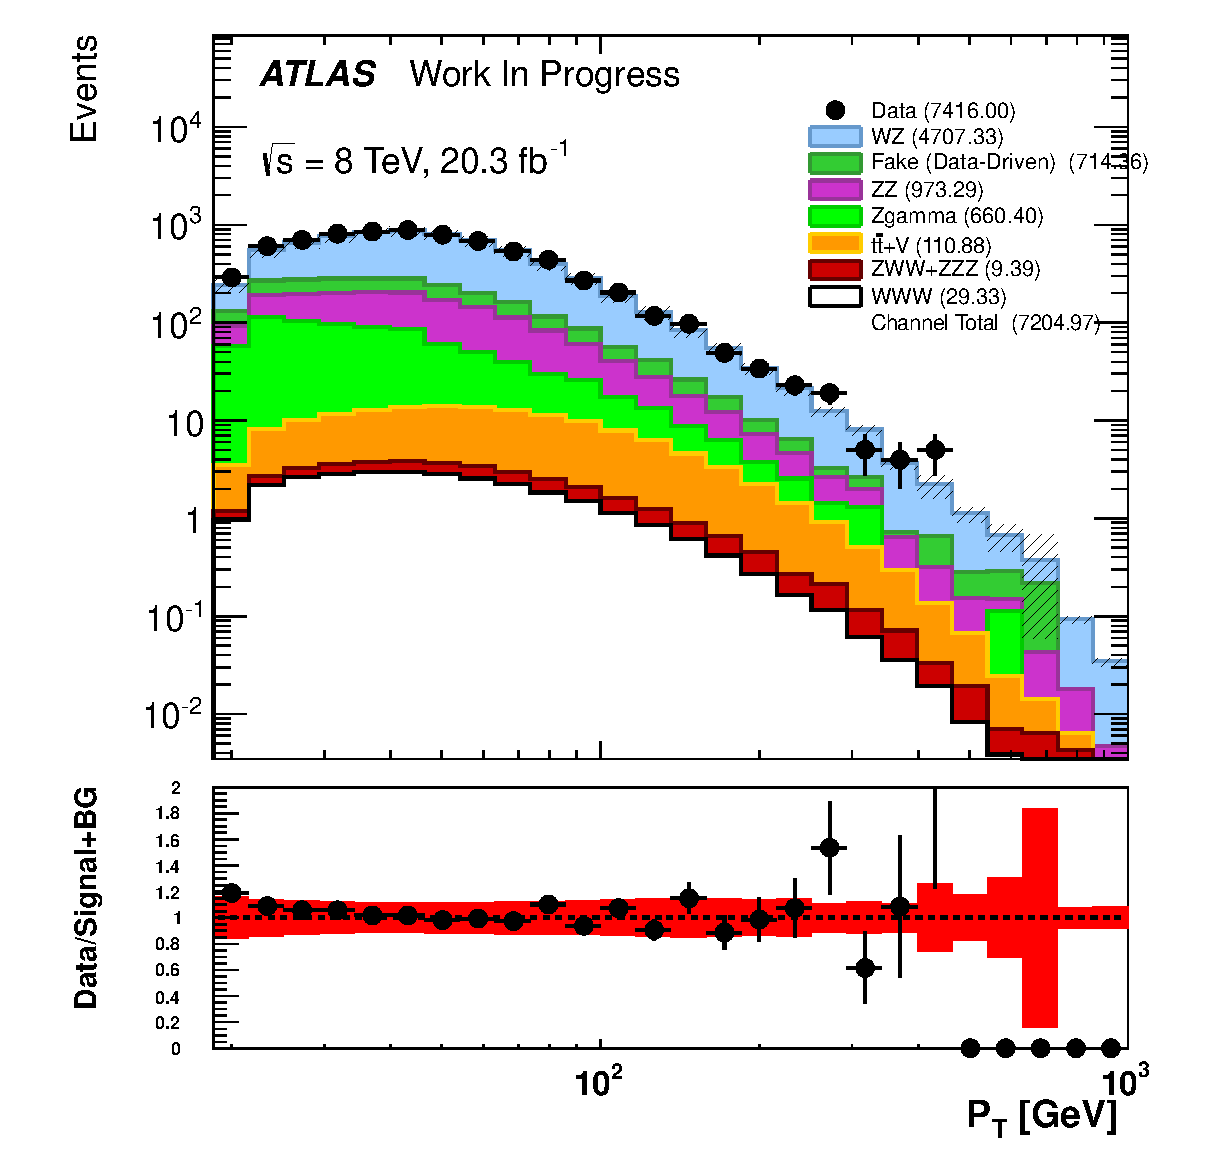
\includegraphics[width=0.3\columnwidth]{figures/appendix_signal_selection/Nov24Update_FakeSys_KFacSys_LogY_NoRebin/output/jobs/MxM/DataFull_Rates_May13_FakeRatesExactly2Loose_MuonMxMBJetGt0_ElBJetGt0SubtractPC_MxM/PreselectionNov23_15_physics/weight_all/eps/AllLeptonPt_histratio.eps}
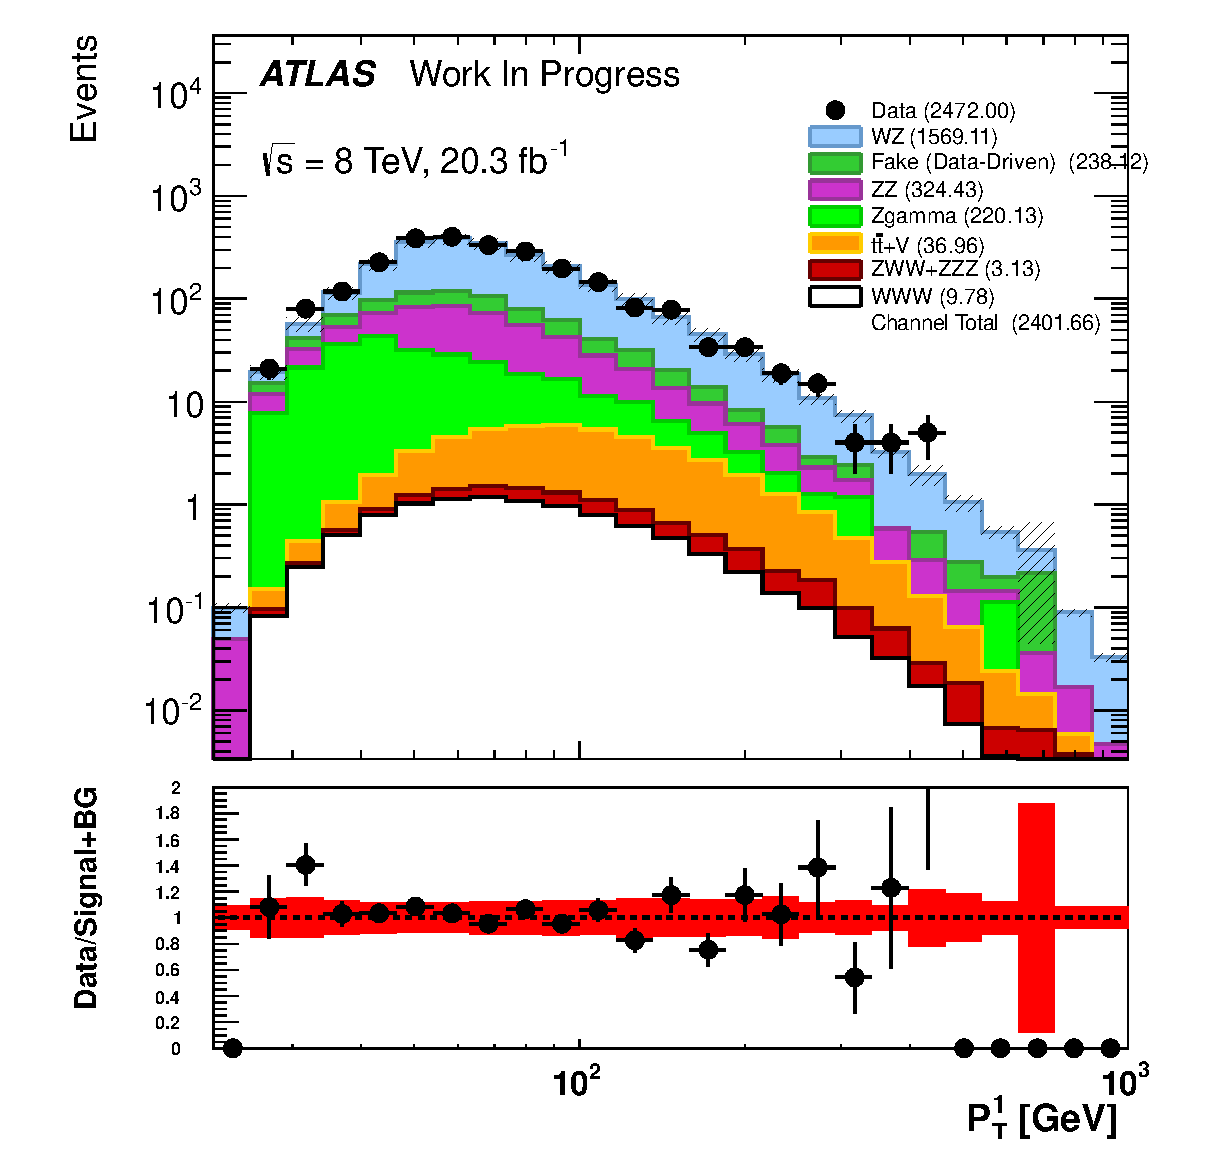
\includegraphics[width=0.3\columnwidth]{figures/appendix_signal_selection/Nov24Update_FakeSys_KFacSys_LogY_NoRebin/output/jobs/MxM/DataFull_Rates_May13_FakeRatesExactly2Loose_MuonMxMBJetGt0_ElBJetGt0SubtractPC_MxM/PreselectionNov23_15_physics/weight_all/eps/LeadingLeptonPt_histratio.eps}
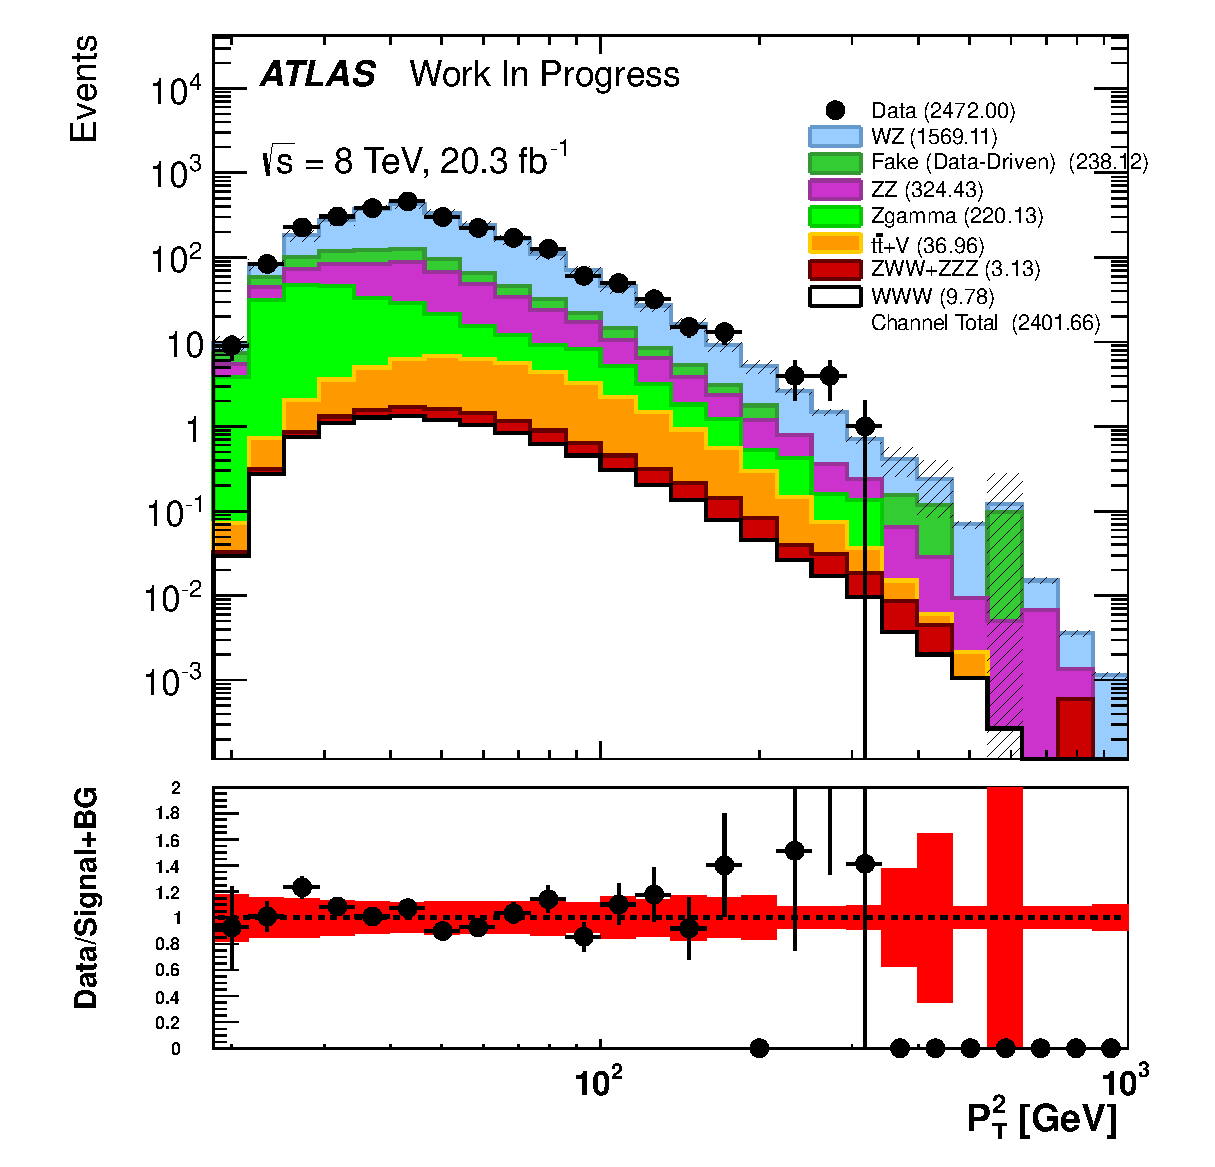
\includegraphics[width=0.3\columnwidth]{figures/appendix_signal_selection/Nov24Update_FakeSys_KFacSys_LogY_NoRebin/output/jobs/MxM/DataFull_Rates_May13_FakeRatesExactly2Loose_MuonMxMBJetGt0_ElBJetGt0SubtractPC_MxM/PreselectionNov23_15_physics/weight_all/eps/SubleadingLeptonPt_histratio.eps}
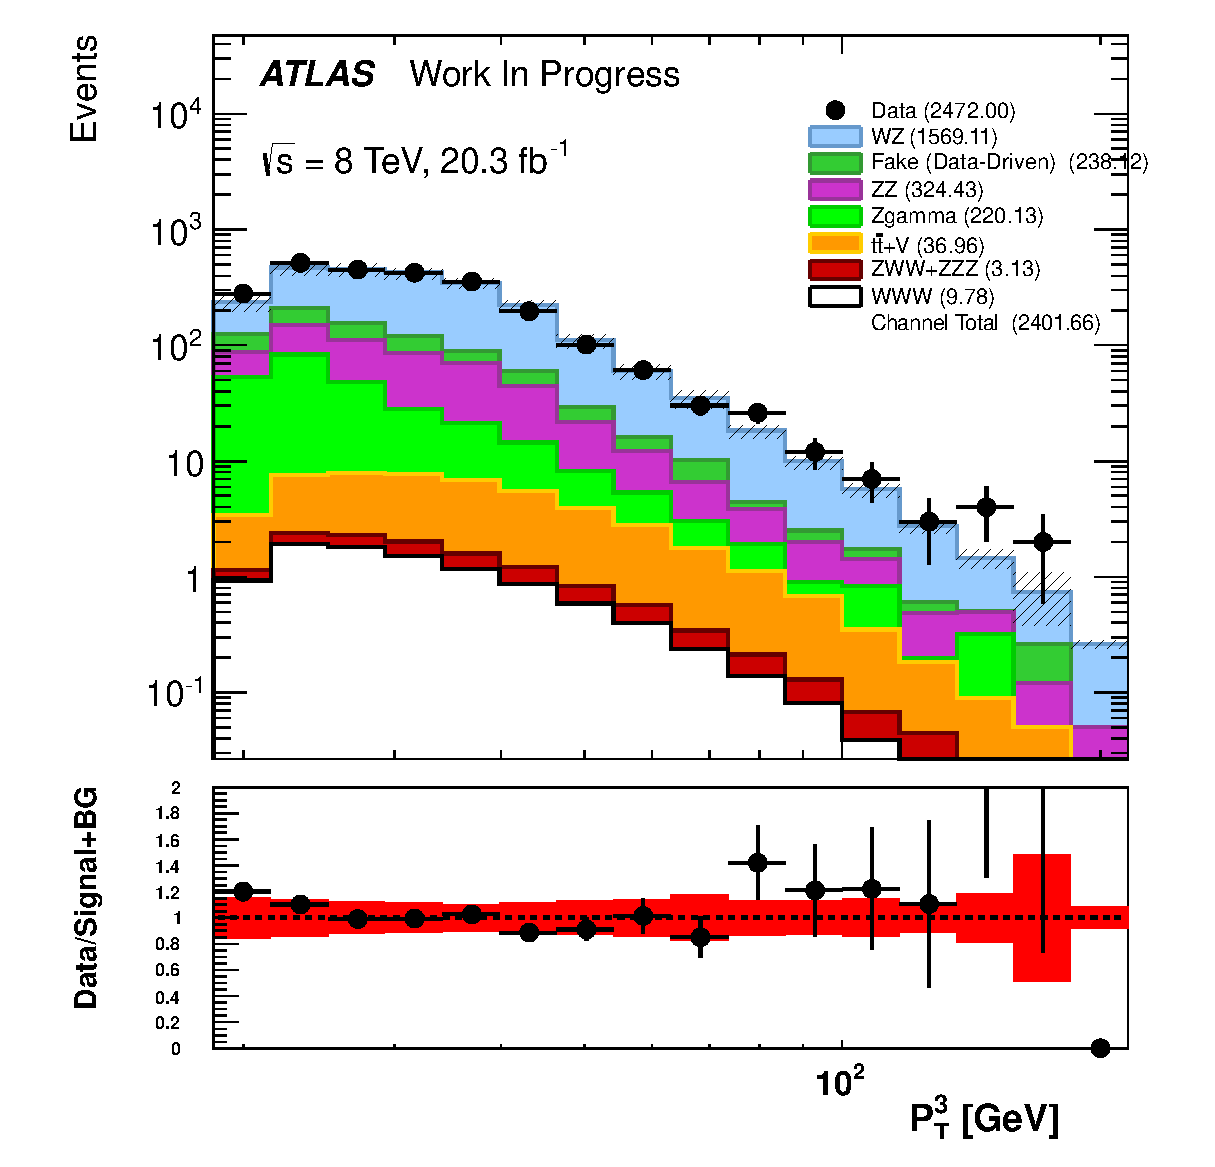
\includegraphics[width=0.3\columnwidth]{figures/appendix_signal_selection/Nov24Update_FakeSys_KFacSys_LogY_NoRebin/output/jobs/MxM/DataFull_Rates_May13_FakeRatesExactly2Loose_MuonMxMBJetGt0_ElBJetGt0SubtractPC_MxM/PreselectionNov23_15_physics/weight_all/eps/MinimumLeptonPt_histratio.eps}
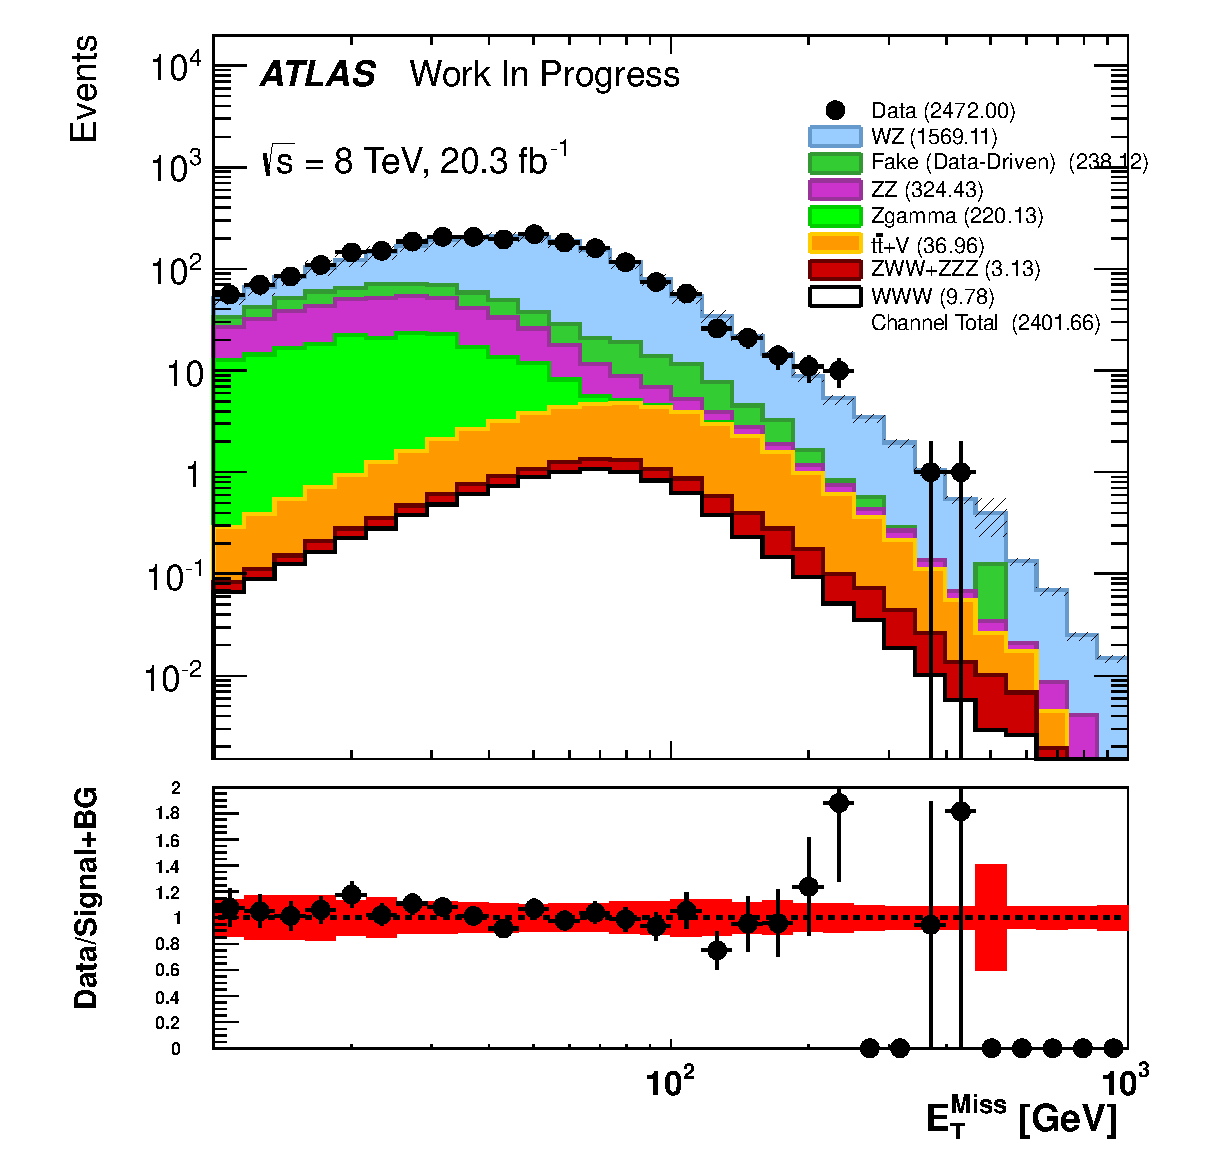
\includegraphics[width=0.3\columnwidth]{figures/appendix_signal_selection/Nov24Update_FakeSys_KFacSys_LogY_NoRebin/output/jobs/MxM/DataFull_Rates_May13_FakeRatesExactly2Loose_MuonMxMBJetGt0_ElBJetGt0SubtractPC_MxM/PreselectionNov23_15_physics/weight_all/eps/MET_Et_histratio.eps}
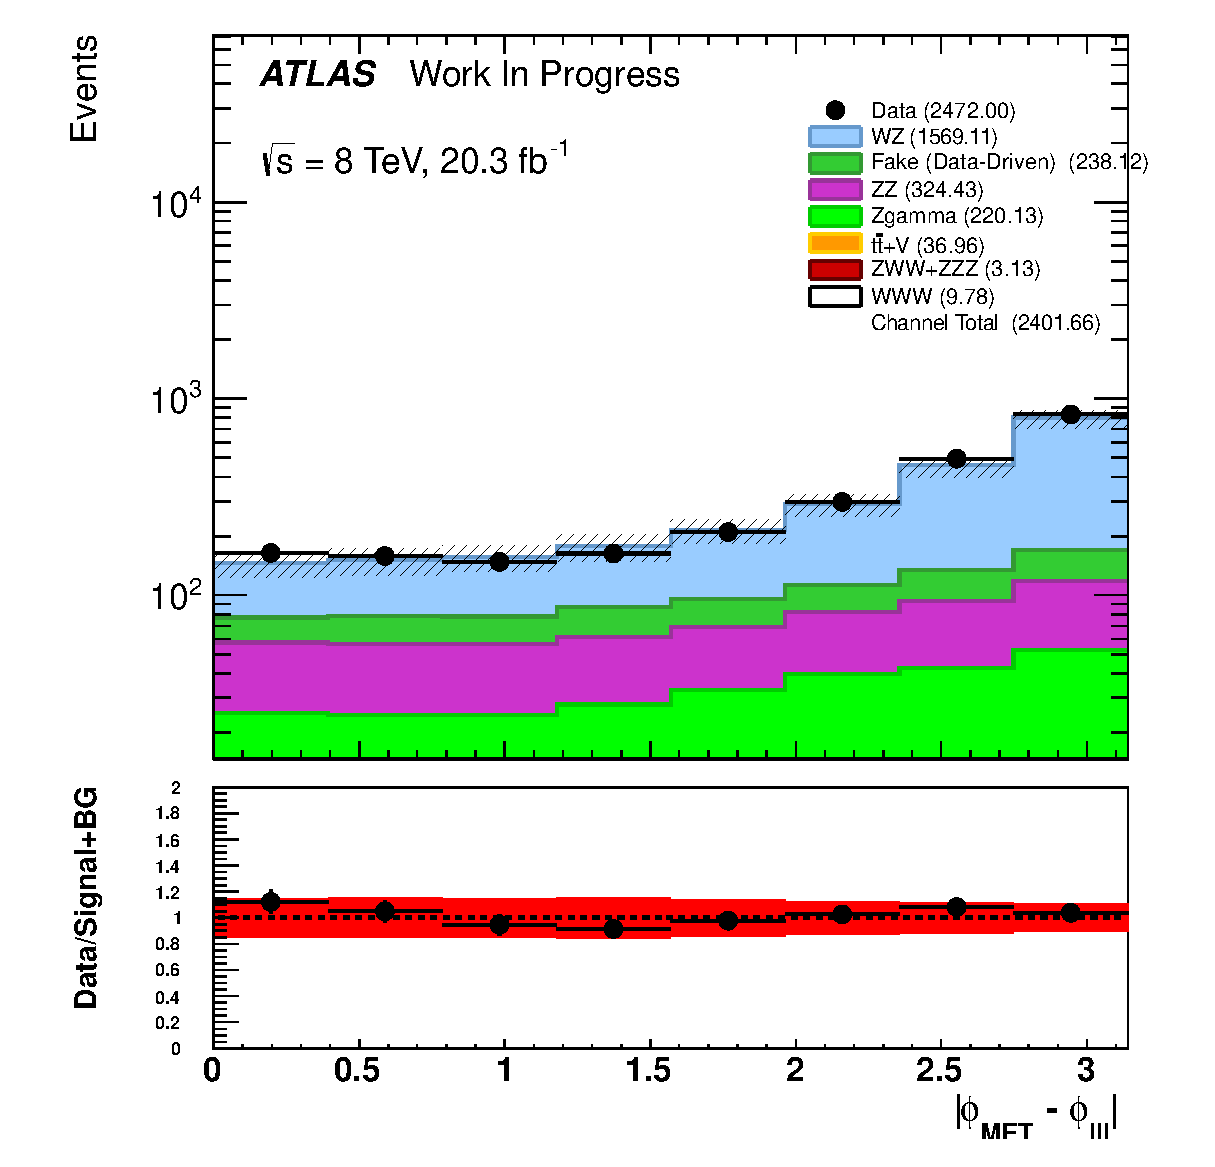
\includegraphics[width=0.3\columnwidth]{figures/appendix_signal_selection/Nov24Update_FakeSys_KFacSys_LogY_NoRebin/output/jobs/MxM/DataFull_Rates_May13_FakeRatesExactly2Loose_MuonMxMBJetGt0_ElBJetGt0SubtractPC_MxM/PreselectionNov23_15_physics/weight_all/eps/DeltaPhiMET123_Abs_histratio.eps}
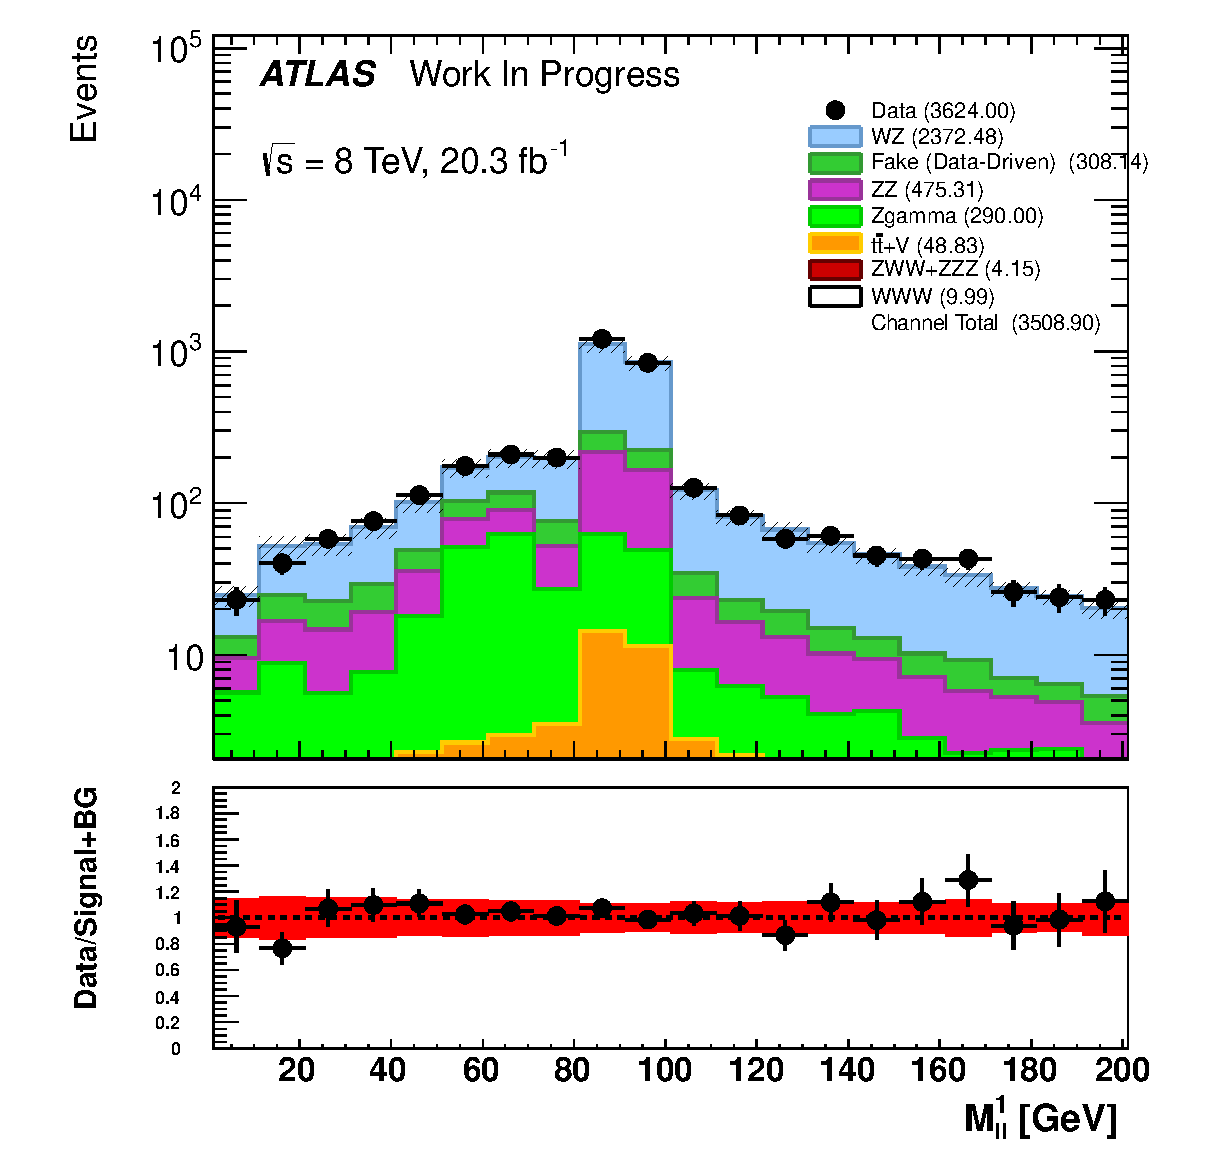
\includegraphics[width=0.3\columnwidth]{figures/appendix_signal_selection/Nov24Update_FakeSys_KFacSys_LogY_NoRebin/output/jobs/MxM/DataFull_Rates_May13_FakeRatesExactly2Loose_MuonMxMBJetGt0_ElBJetGt0SubtractPC_MxM/PreselectionNov23_15_physics/weight_all/eps/InvariantMassSFOS_histratio.eps}
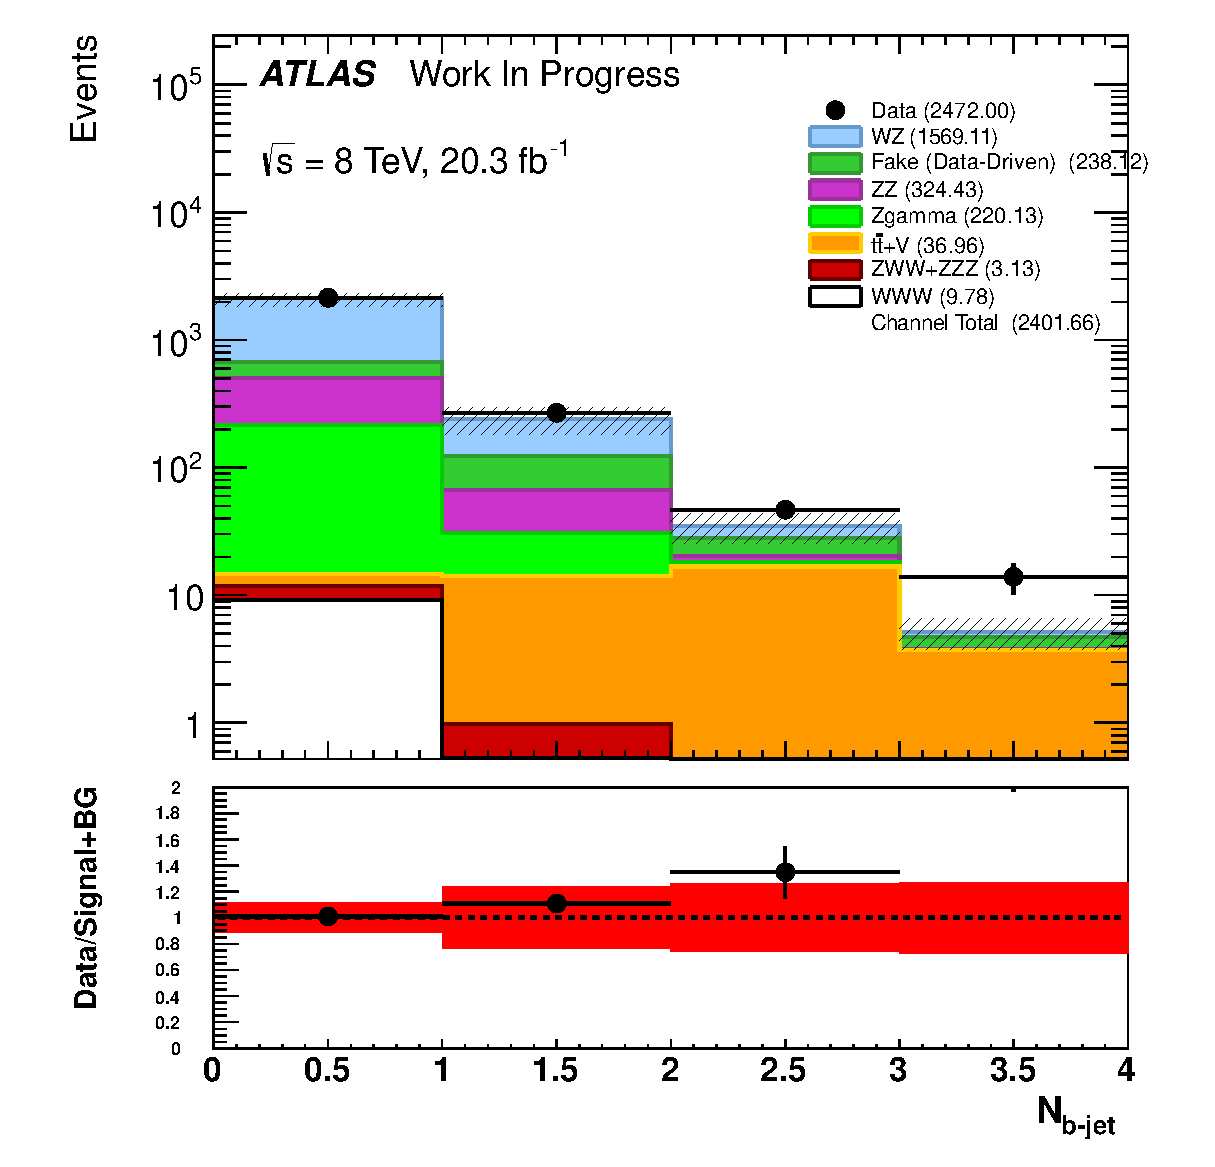
\includegraphics[width=0.3\columnwidth]{figures/appendix_signal_selection/Nov24Update_FakeSys_KFacSys_LogY_NoRebin/output/jobs/MxM/DataFull_Rates_May13_FakeRatesExactly2Loose_MuonMxMBJetGt0_ElBJetGt0SubtractPC_MxM/PreselectionNov23_15_physics/weight_all/eps/NBTaggedJets_histratio.eps}
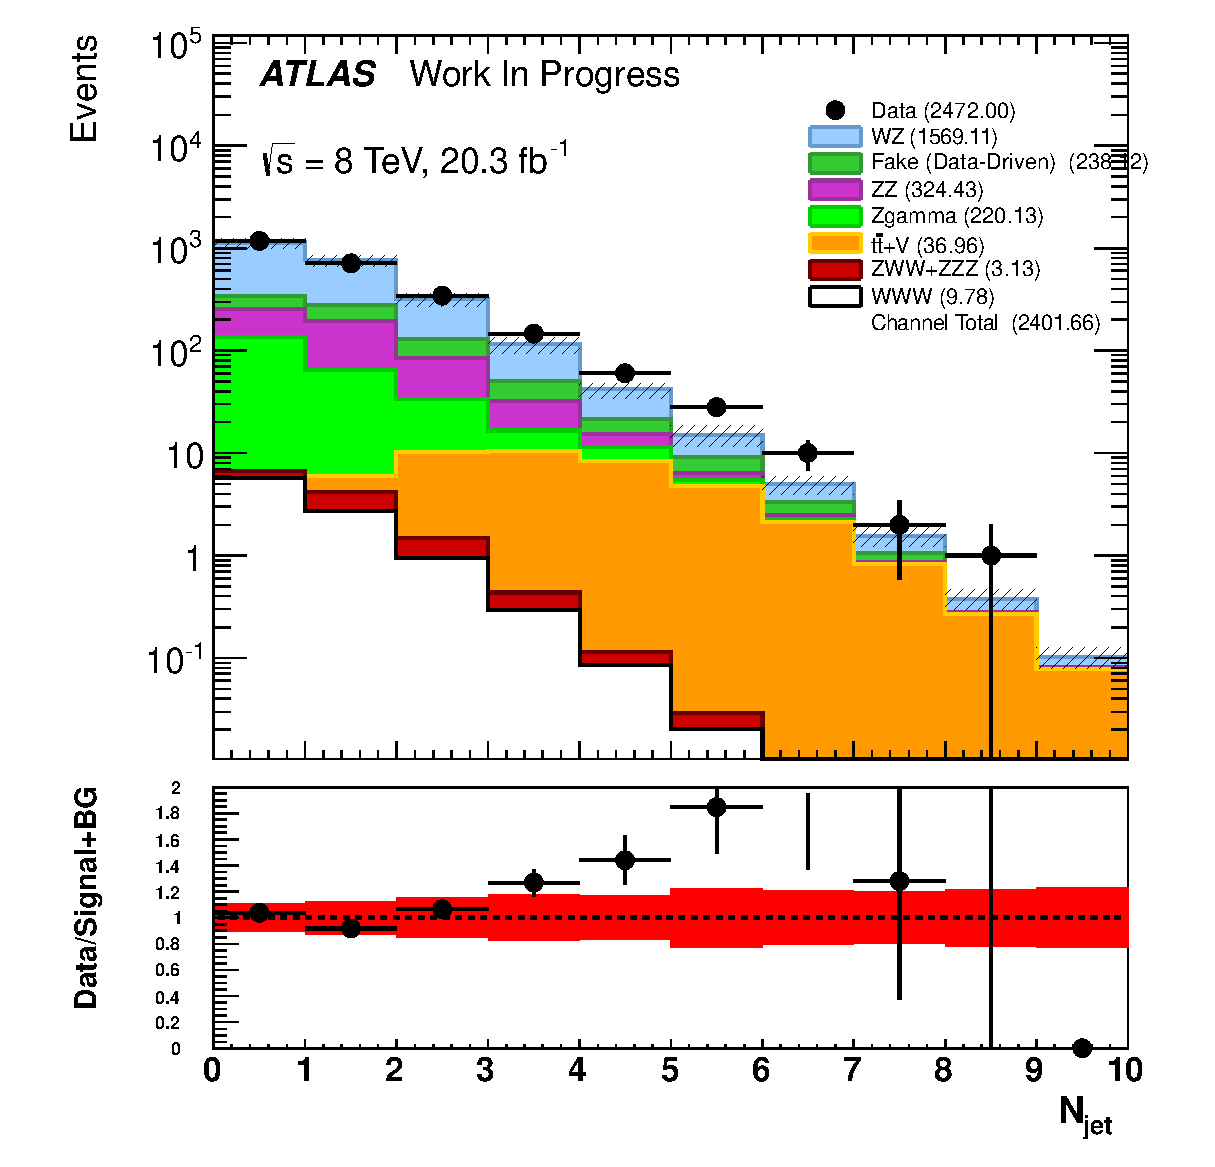
\includegraphics[width=0.3\columnwidth]{figures/appendix_signal_selection/Nov24Update_FakeSys_KFacSys_LogY_NoRebin/output/jobs/MxM/DataFull_Rates_May13_FakeRatesExactly2Loose_MuonMxMBJetGt0_ElBJetGt0SubtractPC_MxM/PreselectionNov23_15_physics/weight_all/eps/NJets_histratio.eps}
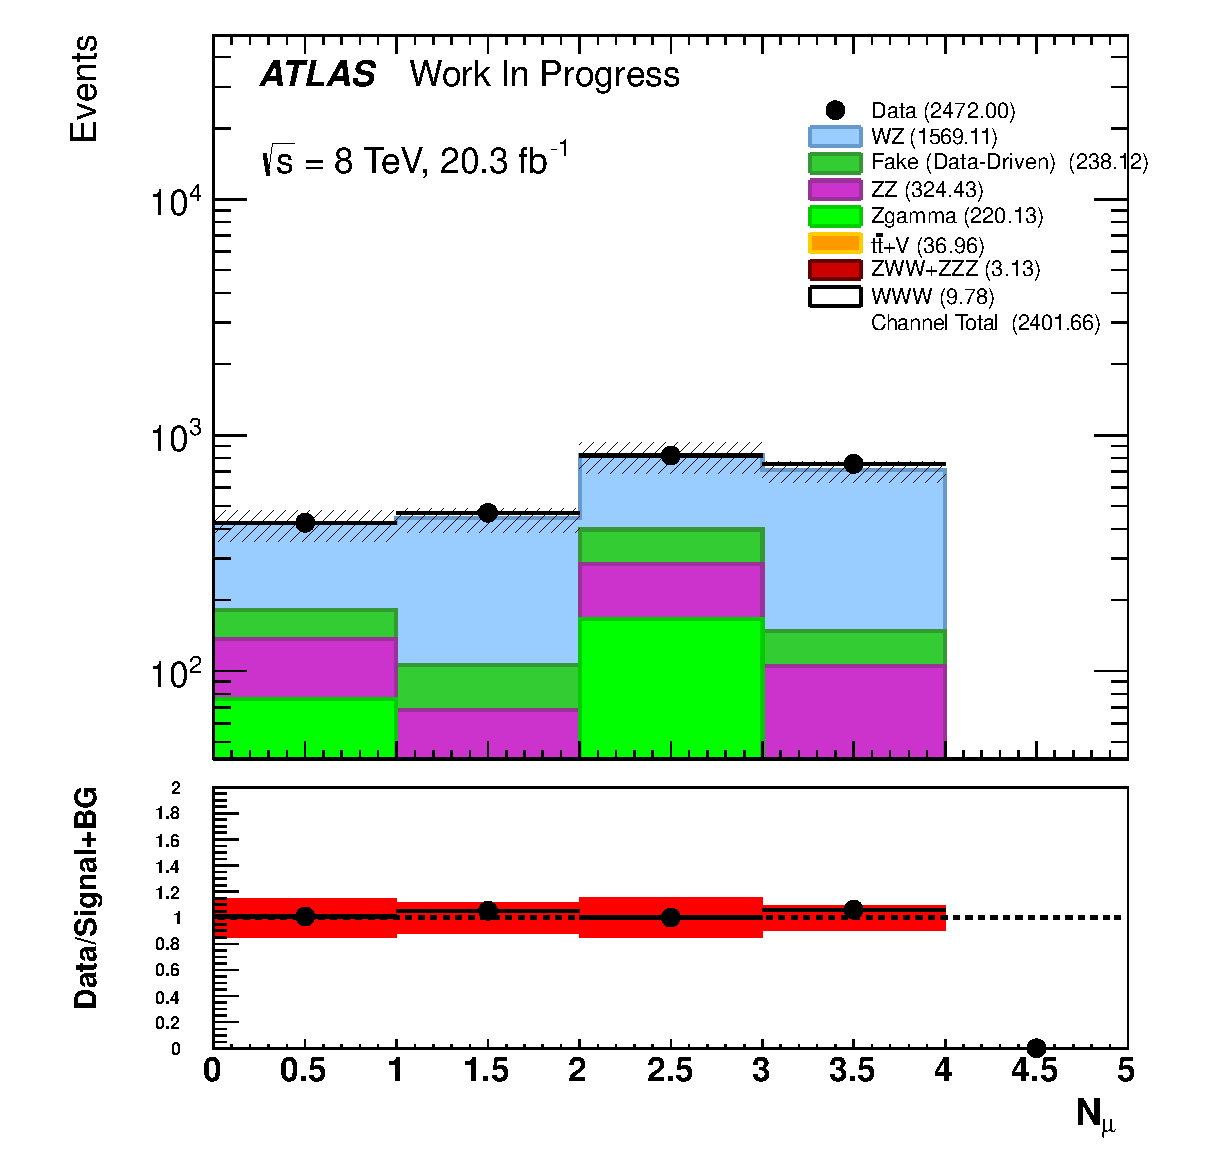
\includegraphics[width=0.3\columnwidth]{figures/appendix_signal_selection/Nov24Update_FakeSys_KFacSys_LogY_NoRebin/output/jobs/MxM/DataFull_Rates_May13_FakeRatesExactly2Loose_MuonMxMBJetGt0_ElBJetGt0SubtractPC_MxM/PreselectionNov23_15_physics/weight_all/eps/NMuons_histratio.eps}
%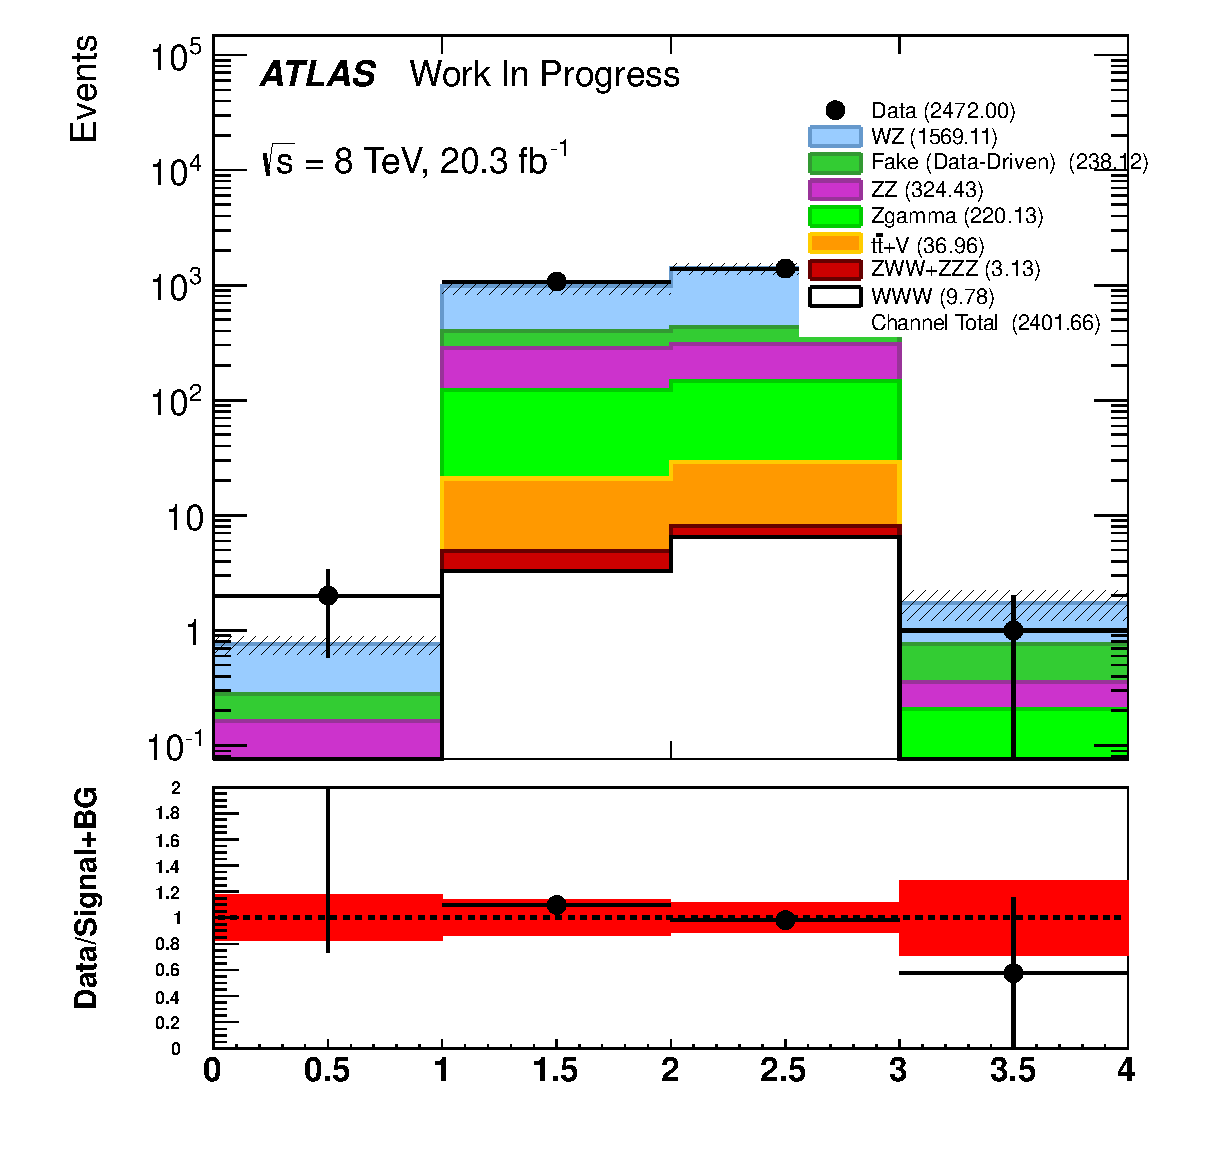
\includegraphics[width=0.3\columnwidth]{figures/appendix_signal_selection/Nov24Update_FakeSys_KFacSys_LogY_NoRebin/output/jobs/MxM/DataFull_Rates_May13_FakeRatesExactly2Loose_MuonMxMBJetGt0_ElBJetGt0SubtractPC_MxM/PreselectionNov23_15_physics/weight_all/eps/TotalCharge_histratio.eps}
\caption{Distributions showing the observed data compared to the background estimate at event pre-selection.
From top to bottom and left to right, these distributions are: the leading, 
sub-leading, and minimum lepton \pt~(ordered by their \pt), 
\MET, \deltaphi, $m_{\textrm{SFOS}}$, \njet, \nbjet, and $N_{\mu}$.
}
\label{fig:preselection}
\end{figure}
The signal plus background model 
(described in detail in \sec\ref{sec:bg_estimates})
is compared to data at pre-selection, defined in \sec\ref{sec:preselection},
for a few different kinematic distributions 
in \fig\ref{fig:preselection}. In the upper plot of each distribution,
the colored histograms 
represent the different categories contributing to the signal 
plus background model and 
are split by color based on the category. 
%The colors are...
Hashed bands are shown on the stacked
histograms representing the size of the systematic uncertainties 
on the model, described in \sec\ref{sec:systematics}.
The data is shown in the black points where the 
bars on the points represent the statistical uncertainty on the data.
The lower plot shows the ratio of the data over the model.
In this case, the error bars correspond to the statistical uncertainty
on the ratio due to both the data and the model. The red band
shows the size of the systematic uncertainties with respect to the model.
The model is said to be consistent with the data
if the ratio is compatible with unity after considering statistical
and systematic uncertainties.
The different distributions are chosen primarily because 
of their potential to discriminate between signal and background. 
The signal plus background model is observed to be consistent
with the data at pre-selection. 




%\begin{table}[ht!]
%\centering
%\begin{tabular}{|c||c|c|c|c|}
\hline
 & $eee$ & $ee\mu$ & $e\mu\mu$ & $\mu\mu\mu$\\ 
\hline\hline
$WZ$ &  $240.85 \pm 0.67$ &  $339.17 \pm 0.82$ &  $422.07 \pm 0.87$ &  $567.0 \pm 1$\\ 
$ZZ$ &  $60.21 \pm 0.13$ &  $54.1 \pm 0.2$ &  $118.60 \pm 0.31$ &  $91.48 \pm 0.17$\\ 
$Z\gamma$ &  $70.1 \pm 2.7$ &  $0.47 \pm 0.22$ &  $149.4 \pm 3.9$ &  $0.17 \pm 0.12$\\ 
$ZWW+ZZZ$ &  $0.436 \pm 0.019$ &  $0.834 \pm 0.027$ &  $1.00 \pm 0.03$ &  $0.864 \pm 0.028$\\ 
$t\bar{t}+V$ &  $4.854 \pm 0.044$ &  $9.549 \pm 0.064$ &  $12.047 \pm 0.072$ &  $10.510 \pm 0.066$\\ 
Fake (data-driven) &  $45.1 \pm 2.2$ &  $37.8 \pm 1.6$ &  $112.7 \pm 2.8$ &  $42.5 \pm 1.2$\\ 
$WWW$ &  $0.770 \pm 0.011$ &  $3.023 \pm 0.023$ &  $3.970 \pm 0.026$ &  $1.843 \pm 0.018$\\ 
\hline
Expected Background &  $421.6 \pm 3.5$ &  $441.9 \pm 1.8$ &  $815.8 \pm 4.9$ &  $712.5 \pm 1.6$\\ 
Expected Signal + Background &  $422.4 \pm 3.5$ &  $444.9 \pm 1.8$ &  $819.8 \pm 4.9$ &  $714.4 \pm 1.6$\\ 
\hline
Observed Data &  $426 \pm 21$ &  $468 \pm 22$ &  $821 \pm 29$ &  $757 \pm 28$\\ 
\hline
\end{tabular}

%\caption{Expected and observed event yields binned by lepton flavor combination at event pre-selection.
%Only statistical uncertainties are shown.
%}
%\label{tab:preselection}
%\end{table}



\begin{figure}[ht!]
\centering
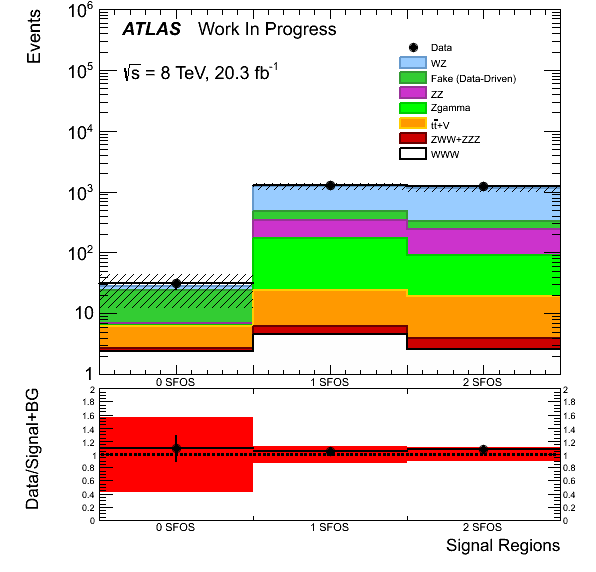
\includegraphics[width=0.5\columnwidth]{figures/SFOSPreselection.png}
\caption{Yields at event pre-selection in the 0, 1 and 2 SFOS regions.  
The most important systematic uncertainties 
(discussed in section~\ref{sec:systematics}) are shown, 
namely from the fake estimates and the uncertainties on the WZ and ZZ k-factors.}
\label{fig:preselection_nsfos}
\end{figure}

Upon splitting the pre-selection region based on the number of SFOS
pairs, we end up with the signal and background predictions in
\fig\ref{fig:preselection_nsfos}, where we can see differences
in the branching fraction for the signal to fall into
each of the three signal regions.
In the 0 and 2 SFOS regions, roughly 2.5 signal events are predicted
whereas closer to 5 signal events are predicted in the 1 SFOS region,
totaling about 10 signal events predicted at the pre-selection stage.
Shifting to looking at the background, perhaps the most striking 
feature of this plot is the 
clear difference in background yield and background composition
between the 0 SFOS region and the 1 and 2 SFOS regions.
More than 1000 background events are predicted in both the 1 and
the 2 SFOS regions, but only about 30 background events are
predicted in the 0 SFOS region.
Clearly then, the advantage of splitting the signal region based on this
classification comes when looking at the background, specifically the
electroweak $WZ$ and $ZZ$ backgrounds where SFOS lepton pairs may be
produced from the decay of the $Z$ boson(s). Consider only the case
where the $WZ$ and $ZZ$ decay to either $e$ or $\mu$.  The $WZ$ production
process is thus characterized by 3 leptons with at least 1 SFOS lepton pair
which comes from the $Z$. If all three leptons from the $WZ$ decay have been
reconstructed, then there is a 50~\% chance the third lepton 
will also be able to form a SFOS pair with one of the leptons from the $Z$ decay.
Thus, the WZ background will split evenly between the 1 and 2 SFOS classification.
Something similar occurs for the ZZ background except that the fourth lepton 
in the decay must be lost (usually due to possessing a low $\pt$).
The large cross-section for these processes means that
they become the dominant backgrounds in the 1 and 2 SFOS regions.  
The 0 SFOS signal region is mostly spared from contamination  by 
these large processes but still
includes both the $WZ$ and $ZZ$ processes as background due to the
non-negligible (albeit small) effect of mis-measurement of the electron
charge described in \sec\ref{sec:charge_misid}.  The 0 SFOS signal region
is thus unique in having a small background which is almost entirely
reducible and dominated instead by the fake background,
described in \sec\ref{sec:bg_fake},
along with the aforementioned sub-dominant effect of electron charge 
mis-identification.

\subsection{Optimization}
\label{sec:optimization}

A more stringent selection must be applied on top of the pre-selection
in \sec\ref{sec:preselection_yield} in order to obtain any
sensitivity to the signal.  The best selection, however, is
not known \emph{a priori}. We try to find the best possible selection
by starting from a list of kinematic quantities, chosen based on heuristic
arguments. These kinematic quantities, along with the signal
plus background model, are passed into an optimization 
framework that systematically seeks to simultaneously 
maximize the predicted signal and the precision on the final measurement.

The optimization framework considers independent permutations of the different
kinematic quantities, along with variations of the selection thresholds
on these cuts, to form combinations of selection cuts which could become a final
selection. For each combination, or operating point,
that is considered, the signal plus background
model is evaluated to determine the expected yields and systematic
uncertainties given that selection.  The LHC data is not used in the optimization.  
The prediction is then plugged into the statistical framework described in
\sec\ref{sec:measurement} to extract a value on the expected precision
of the measurement. For each operating point,
the value on the precision is plotted against the expected signal yield.
With some discretion, we then choose the operating point 
that maximized the signal yield and gives the smallest absolute 
precision on the measurement. 


The selection thresholds considered are...

We split by signal region...

The different operating points look like...


Some of the intuition for this can be understood by looking at individual
distributions...

this results in the selection of table blah...

\subsection{Signal Region Yields}
\label{sec:signal_yield}
\begin{figure}[ht!]
\centering
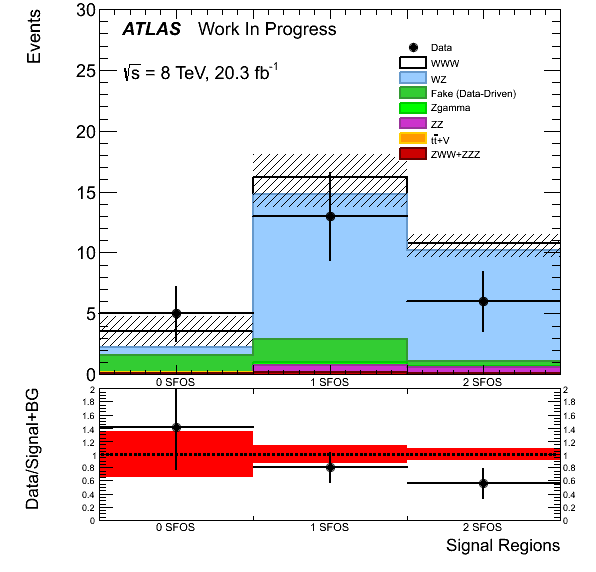
\includegraphics[width=0.5\columnwidth]{figures/SFOSSignalRegions.png}
\caption{Yields after full selection in the 0, 1 and 2 SFOS regions.  
The most important systematic uncertainties are shown, namely from the 
fake estimates and the uncertainties on the WZ and ZZ k-factors.}
\label{fig:sig_yields_nsfos}
\end{figure}

The optmized signal region selection
described in \sec\ref{sec:optimization} and \sec\ref{sec:signal_regions}
and listed in \tab\ref{tab:signal_selection} is applied 
to the data as well as the signal plus background model.
A plot of the predicted yields for the 
signal plus background, along with systematic uncertainties,
is compared to the data for each signal region
in \fig\ref{fig:sig_yields_nsfos}. A detailed 
breakdown of the predicted yields and overall uncertainties
on each background as well as the signal prediction and observed
data
are presented in \tab\ref{tab:sys_summary}.
A breakdown of the systematic uncertainty contributions
to the signal and the backgrounds in each signal region
are summarized in \tab\ref{tab:sys_breakdown}.
More details are presented about each signal region below.



\begin{table}[ht!]
\centering
\renewcommand{\tabcolsep}{2pt}
\small\begin{tabular}{c|rclrclrcl}
\hline
\hline
 & \multicolumn{3}{c}{0 SFOS} & \multicolumn{3}{c}{1 SFOS} & \multicolumn{3}{c}{2 SFOS}\\ 
\hline
$WZ$ &  $0.6176 $&$\pm$&$ 0.0043~^{+0.0699}_{-0.0701}$ &  $11.89 $&$\pm$&$ 0.14~^{+1.32}_{-1.29}$ &  $9.05 $&$\pm$&$ 0.13~^{+0.99}_{-1.00}$\\ 
ZZ &  $0.0658 $&$\pm$&$ 0.0039~^{+0.0112}_{-0.0112}$ &  $0.581 $&$\pm$&$ 0.016~^{+0.106}_{-0.105}$ &  $0.477 $&$\pm$&$ 0.011~^{+0.095}_{-0.086}$\\ 
$WWZ+WZZ$ &  $0.1126 $&$\pm$&$ 0.0099~^{+0.0146}_{-0.0117}$ &  $0.140 $&$\pm$&$ 0.011~^{+0.015}_{-0.013}$ &  $0.0785 $&$\pm$&$ 0.0080~^{+0.0097}_{-0.0106}$\\ 
$t\overline{t}+$V &  $0.0388 $&$\pm$&$ 0.0043~^{+0.0061}_{-0.0077}$ &  $0.0503 $&$\pm$&$ 0.0048~^{+0.0074}_{-0.0089}$ &  $0.0239 $&$\pm$&$ 0.0033~^{+0.0074}_{-0.0058}$\\ 
DPS &  $0.0 $&$\pm$&$ 0.0~^{+0.0}_{-0.0}$ &  $0.0088 $&$\pm$&$ 0.0080~^{+0.0080}_{-0.0084}$ &  $0.023 $&$\pm$&$ 0.016~^{+0.019}_{-0.029}$\\ 
$Z\gamma$ &  $0.0 $&$\pm$&$ 0.0~^{+0.0}_{-0.0}$ &  $0.20 $&$\pm$&$ 0.13~^{+0.29}_{-0.13}$ &  $0.110 $&$\pm$&$ 0.096~^{+0.163}_{-0.288}$\\ 
Fake &  $1.51 $&$\pm$&$ 0.26~^{+1.40}_{-1.29}$ &  $1.90 $&$\pm$&$ 0.34~^{+1.90}_{-1.77}$ &  $0.49 $&$\pm$&$ 0.16~^{+0.47}_{-0.46}$\\ 
Signal &  $1.320 $&$\pm$&$ 0.015~^{+0.072}_{-0.078}$ &  $1.369 $&$\pm$&$ 0.015~^{+0.072}_{-0.080}$ &  $0.603 $&$\pm$&$ 0.010~^{+0.031}_{-0.035}$\\ 
\hline
Total Background &  $2.35 $&$\pm$&$ 0.26~^{+1.40}_{-1.30}$ &  $14.77 $&$\pm$&$ 0.39~^{+2.36}_{-2.22}$ &  $10.25 $&$\pm$&$ 0.23~^{+1.15}_{-1.22}$\\ 
Total Predicted &  $3.67 $&$\pm$&$ 0.26~^{+1.41}_{-1.30}$ &  $16.14 $&$\pm$&$ 0.39~^{+2.33}_{-2.18}$ &  $10.86 $&$\pm$&$ 0.23~^{+1.12}_{-1.19}$\\ 
\hline
Data &  \multicolumn{3}{c}{$5$} &  \multicolumn{3}{c}{$13$} &  \multicolumn{3}{c}{$6$}\\ 
\hline
\end{tabular}

\caption{A summary of the expected yields compared to data for all 
three signal regions.  Statistical uncertainties are shown 
as a symmetric uncertainty on the central value. Systematic uncertainties 
are shown as an asymmetric uncertainty and are shown
after taking the quadrature sum of all individual uncertainties. 
In the actual analysis, each systematic uncertainty is
treated as an individual nuisance paramter and are NOT added in quadrature.  
The presentation here serves only as a demonstration
of the overall size of the systematic uncertainties for each source in the 
individual signal regions.}
\label{tab:sys_summary}
\end{table}

\begin{table}[ht!]
\centering
\small
\renewcommand{\arraystretch}{1.5}
\begin{tabular}{c||ccc|ccc}
\hline

\multirow{2}{*}{Source of Uncertainty} & \multicolumn{3}{|c|}{Signal} & \multicolumn{3}{c}{Backgound} \\
 & 0 SFOS& 1 SFOS & 2 SFOS & 0 SFOS & 1 SFOS & 2 SFOS\\ 
\hline\hline
Electron &  $^{+1.56}_{-1.47}$  &  $^{+1.66}_{-1.61}$  &  $^{+1.02}_{-1.06}$  &  $^{+0.68}_{-0.69}$  &  $^{+2.34}_{-1.49}$  &  $^{+1.05}_{-1.54}$ \\ 
Muon &  $^{+0.56}_{-0.54}$  &  $^{+0.54}_{-0.54}$  &  $^{+0.74}_{-0.83}$  &  $^{+0.19}_{-0.19}$  &  $^{+1.09}_{-0.48}$  &  $^{+0.81}_{-0.80}$ \\ 
MET &  $^{+1.38}_{-1.75}$  &  $^{+0.71}_{-0.89}$  &  $^{+0.23}_{-0.35}$  &  $^{+0.79}_{-0.73}$  &  $^{+1.38}_{-0.11}$  &  $^{+2.12}_{-2.66}$ \\ 
Jet &  $^{+2.36}_{-2.26}$  &  $^{+2.06}_{-2.34}$  &  $^{+1.56}_{-2.22}$  &  $^{+1.10}_{-1.06}$  &  $^{+2.74}_{-2.03}$  &  $^{+2.94}_{-4.41}$ \\ 
Trigger &  $^{+0.09}_{-0.09}$  &  $^{+0.09}_{-0.09}$  &  $^{+0.20}_{-0.20}$  &  $^{+0.06}_{-0.06}$  &  $^{+0.09}_{-0.09}$  &  $^{+0.21}_{-0.21}$ \\ 
Matrix Method & --- & --- & --- &  $^{+58.56}_{-53.98}$  &  $^{+12.64}_{-11.78}$  &  $^{+4.34}_{-4.23}$ \\ 
Charge Mis-ID & --- & --- & --- &  $^{+0.45}_{-0.44}$  & --- & ---\\ 
Pileup &  $^{+0.92}_{-0.77}$  &  $^{+1.10}_{-1.30}$  &  $^{+1.50}_{-1.24}$  &  $^{+0.52}_{-0.42}$  &  $^{+0.22}_{+0.00}$  &  $^{+1.39}_{-1.40}$ \\ 
Luminosity &  $^{+2.80}_{-2.80}$  &  $^{+2.80}_{-2.80}$  &  $^{+2.80}_{-2.80}$  &  $^{+2.80}_{-2.80}$  &  $^{+2.80}_{-2.80}$  &  $^{+2.80}_{-2.80}$ \\ 
Theory &  $^{+5.55}_{-3.75}$  &  $^{+5.55}_{-3.75}$  &  $^{+5.55}_{-3.75}$  &  $^{+2.66}_{-2.66}$  &  $^{+8.07}_{-8.07}$  &  $^{+8.85}_{-8.85}$ \\ 
Statistical &  $^{+1.14}_{-1.14}$  &  $^{+1.12}_{-1.12}$  &  $^{+1.70}_{-1.70}$  &  $^{+10.99}_{-10.99}$  &  $^{+2.67}_{-2.67}$  &  $^{+2.20}_{-2.20}$ \\ 
\hline
\end{tabular}

\caption{Categorized systematic uncertainties 
for signal and background predictions in all three signal regions.
All uncertainties are shown as a percentage of the nominal
prediction.  }
\label{tab:sys_breakdown}
\end{table}


\clearpage
\subsubsection{0 SFOS Signal Region}



\begin{table}[ht!]
\centering
\small
\begin{tabular}{l||c|c||c|c||c|c}
\hline
 &                 \multicolumn{2}{c||}{Signal}            &  \multicolumn{2}{c||}{Background} &  \multicolumn{2}{c}{Data} \\
  & Yield & Eff. & Yield & Eff. & Yield & Eff.\\
  \hline\hline
  1. Pre-selection &  $9.78$ & --- &  $2388.48$ & --- & $2472$ &  --- \\ 
  \hline
  2. 0 SFOS &  $2.31$ &  $0.24$ &  $21.36$ &  $0.0089$ & $30$ &  $0.01$\\ 
  \hline
  3. Charge Sum $= \pm 1$ &  $2.30$ &  $1.00$ &  $19.55$ &  $0.92$ & $27$ &  $0.90$\\ 
  \hline
  4. $N_{\mathrm{b-jet}} = 0$ &  $2.29$ &  $0.99$ &  $8.59$ &  $0.44$ & $10$ &  $0.37$\\ 
  \hline
  5. $m_{SF} > 20$ GeV &  $2.25$ &  $0.98$ &  $8.32$ &  $0.97$ & $10$ &  $1.00$\\ 
  \hline
  6. $|m_{ee} - m_{Z}| > 15$ GeV &  $2.06$ &  $0.91$ &  $7.09$ &  $0.85$ & $9$ &  $0.90$\\ 
  \hline
  7. $|\Delta\phi(3l,E_{T}^{Miss})| > 2.5$ &  $1.41$ &  $0.69$ &  $2.51$ &  $0.35$ & $6$ &  $0.67$\\ 
  \hline
  8. $N_{\mathrm{Jet}} \leq 1$ &  $1.34$ &  $0.95$ &  $2.35$ &  $0.94$ & $5$ &  $0.83$\\ 
  \hline
  \end{tabular}


\caption{Cut-flows showing the event yields and efficiencies for each cut in the 0 SFOS signal region
starting from event pre-selection separately for the total signal and total bacgkround predictions, along with the observed data. 
Event yields for MC backgrounds and signal include all weights and are normalized to an integrated luminosity of $20.3~\mathrm{fb}^{-1}$.  
The fake lepton background only includes the matrix method weights.  The data is unweighted.
Efficiencies show the ratio of the yield with respect
to the previous cut.  The efficiency is first calculated at the first cut after event pre-selection.  }
\label{tab:cutflow_weighted_0sfos}
\end{table}

\begin{table}[ht!]
\centering
\small
\begin{tabular}{l||c|c||c|c||c|c}
\hline
 &  \multicolumn{6}{c}{Background} \\
 & \multicolumn{2}{c||}{$WZ$} & \multicolumn{2}{c||}{$ZZ$} & \multicolumn{2}{c}{$t\bar{t}+V$} \\ 
 & Yield & Eff. & Yield & Eff. & Yield & Eff. \\
\hline\hline
Pre-selection &  $1566.91$ & --- &  $323.60$ &  --- &  $36.93$ &  --- \\
\hline
0 SFOS &  $2.84$ &  $0.002$ &  $0.50$ &  $0.002$ &  $0.26$ &  $0.01$ \\
\hline
Charge Sum $= \pm 1$ &  $1.92$ &  $0.68$ &  $0.33$ &  $0.65$ &  $0.26$ &  $0.99$ \\
\hline
$N_{\mathrm{b-jet}} = 0$ &  $1.91$ &  $0.99$ &  $0.33$ &  $0.99$ &  $0.25$ &  $0.98$ \\
\hline
$m_{SF} > 20$ GeV &  $1.88$ &  $0.98$ &  $0.32$ &  $0.98$ &  $0.25$ &  $0.98$ \\
\hline
$|m_{ee} - m_{Z}| > 15$ GeV &  $1.27$ &  $0.68$ &  $0.21$ &  $0.66$ &  $0.22$ &  $0.90$ \\
\hline
$|\Delta\phi(3l,E_{T}^{Miss})| > 2.5$ &  $0.65$ &  $0.51$ &  $0.07$ &  $0.34$ &  $0.09$ &  $0.38$ \\
\hline
$N_{\mathrm{Jet}} \leq 1$ &  $0.62$ &  $0.95$ &  $0.07$ &  $0.91$ &  $0.04$ &  $0.45$ \\
\hline
\end{tabular}




\begin{tabular}{l||c|c||c|c||c|c}
\hline
 &  \multicolumn{6}{c}{Background} \\
 & \multicolumn{2}{c||}{$ZZZ+ZWW$} & \multicolumn{2}{c||}{$Z\gamma$} & \multicolumn{2}{c}{Fake}  \\ 
 & Yield & Eff. & Yield & Eff. & Yield & Eff. \\
\hline\hline
Pre-selection &  $3.12$ & --- &  $219.80$ &  --- &  $238.12$ &  --- \\ 
\hline
0 SFOS &  $0.25$ &  $0.08$ &  $0.20$ &  $0.001$ &  $17.31$ &  $0.07$ \\ 
\hline
Charge Sum $= \pm 1$ &  $0.25$ &  $1.00$ &  $0.00$ &  $0.00$ &  $16.79$ &  $0.97$ \\ 
\hline
$N_{\mathrm{b-jet}} = 0$ &$0.25$ &  $0.99$ &  $0.00$ &  $0.00$ &  $5.85$ &  $0.35$ \\ 
\hline
$m_{SF} > 20$ GeV &$0.24$ &  $0.98$ &  $0.00$ &  $0.00$ &  $5.63$ &  $0.96$ \\ 
\hline
$|m_{ee} - m_{Z}| > 15$ GeV &$0.22$ &  $0.90$ &  $0.00$ &  $0.00$ &  $5.17$ &  $0.92$ \\ 
\hline
$|\Delta\phi(3l,E_{T}^{Miss})| > 2.5$ &$0.13$ &  $0.59$ &  $0.00$ &  $0.00$ &  $2.17$ &  $0.42$ \\ 
\hline
$N_{\mathrm{Jet}} \leq 1$ &$0.11$ &  $0.86$ &  $0.00$ &  $0.00$ &  $1.51$ &  $0.70$ \\ 
\hline
\end{tabular}




\caption{Cut-flows showing the event yields and efficiencies for each cut in the 0 SFOS signal region
starting from event pre-selection and binned by background category. 
Event yields for MC backgrounds and signal include all weights and are normalized to an integrated luminosity of $20.3~\mathrm{fb}^{-1}$.  
The fake lepton background only includes the matrix method weights.  The data is unweighted.
Efficiencies show the ratio of the yield with respect
to the previous cut.  The efficiency is first calculated at the first cut after event pre-selection.  }
\label{tab:cutflow_weighted_0sfos_bg}
\end{table}

\begin{figure}[ht!]
\centering
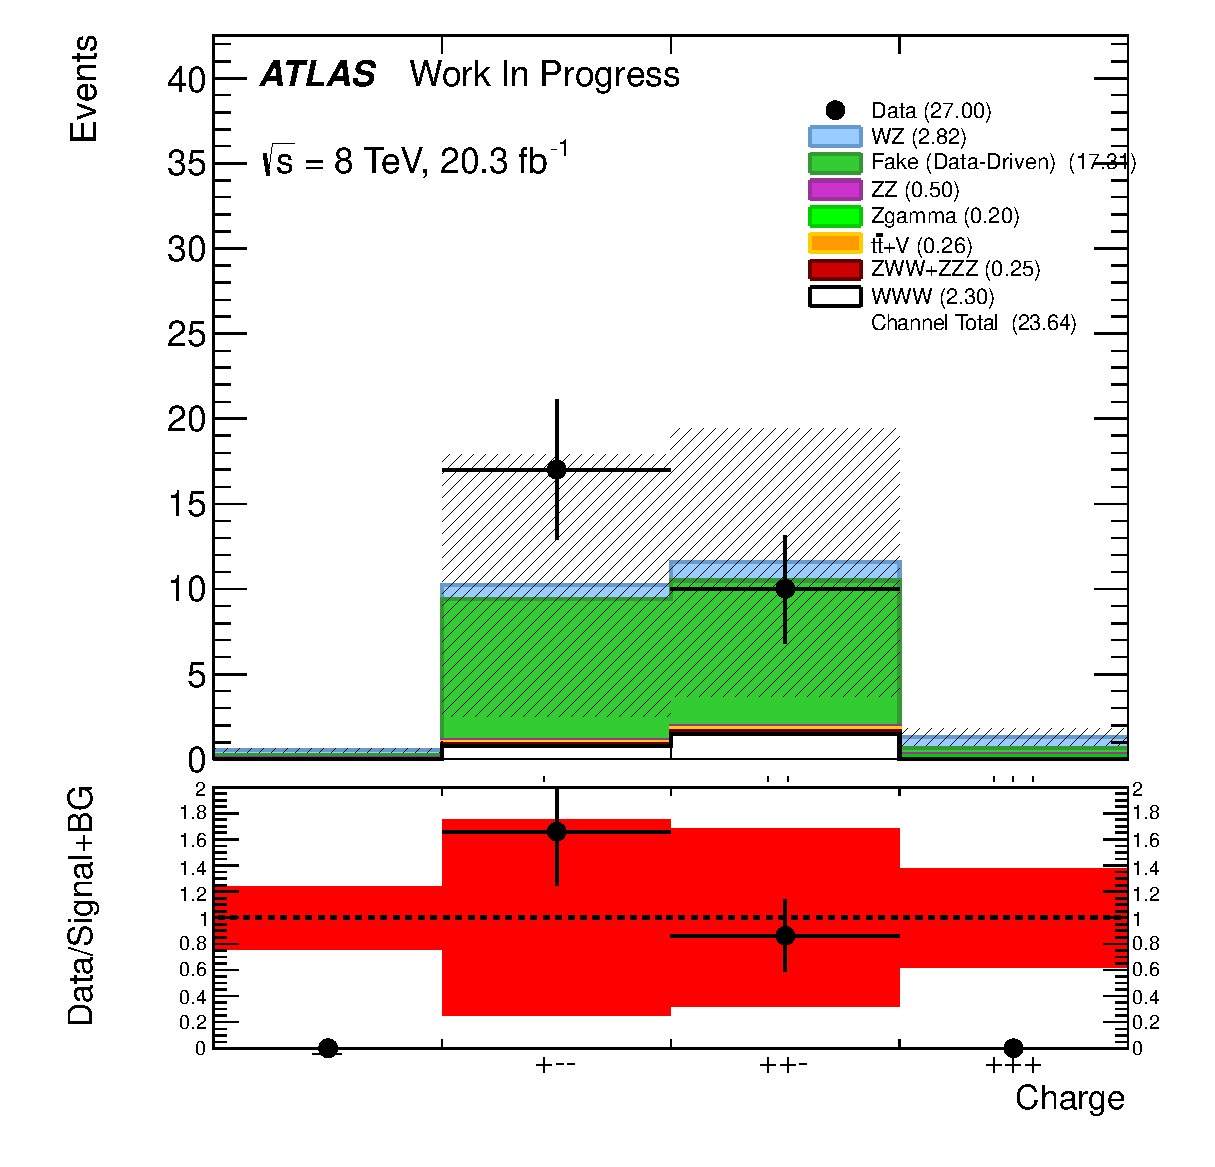
\includegraphics[width=0.3\columnwidth]{figures/appendix_signal_selection/Nov24Update_FakeSys_KFacSys_LinearY_Rebin/output/jobs/MxM/DataFull_Rates_May13_FakeRatesExactly2Loose_MuonMxMBJetGt0_ElBJetGt0SubtractPC_MxM/PreselectionNov23_15_0SFOS_physics/weight_all/eps/TotalCharge_histratio.eps}
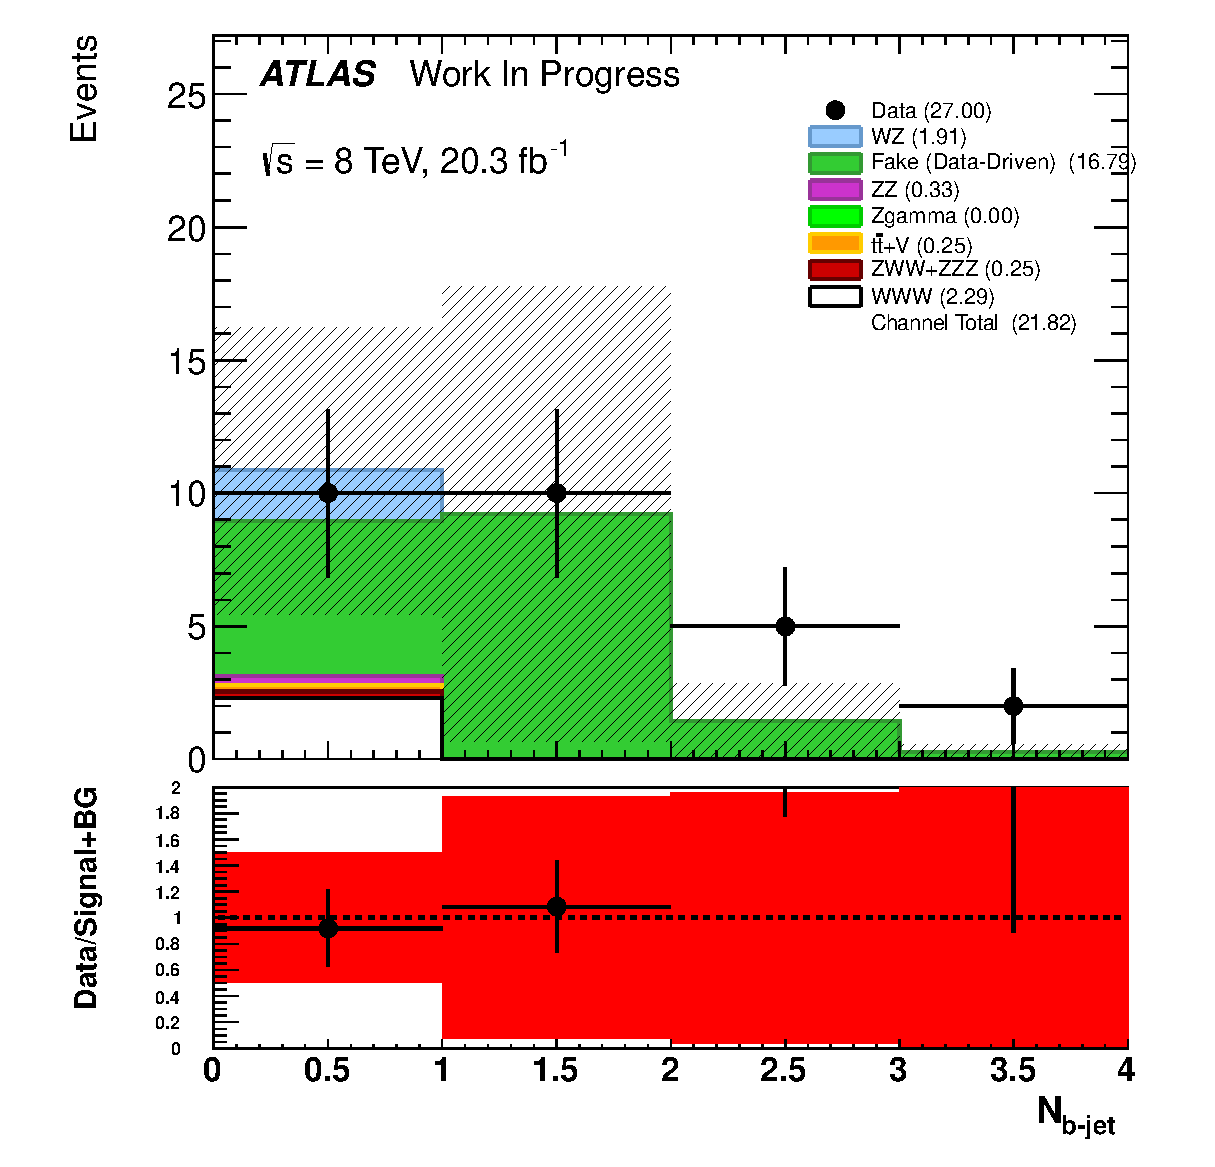
\includegraphics[width=0.3\columnwidth]{figures/appendix_signal_selection/Nov24Update_FakeSys_KFacSys_LinearY_Rebin/output/jobs/MxM/DataFull_Rates_May13_FakeRatesExactly2Loose_MuonMxMBJetGt0_ElBJetGt0SubtractPC_MxM/PreselectionNov23_15_0SFOS_ChargeAbs1_physics/weight_all/eps/NBTaggedJets_histratio.eps}
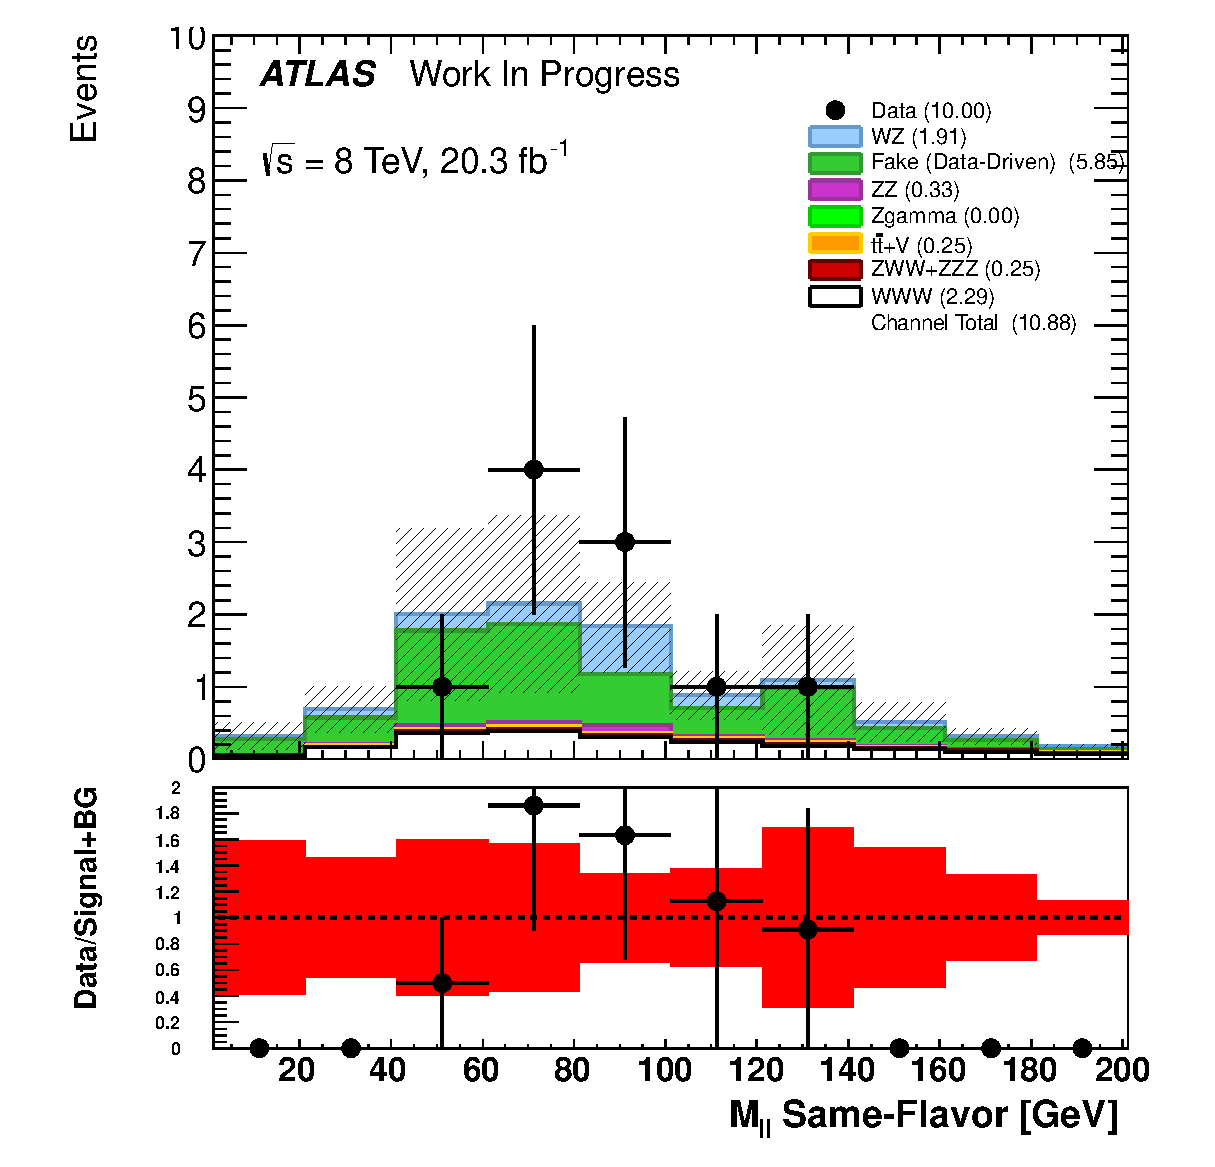
\includegraphics[width=0.3\columnwidth]{figures/appendix_signal_selection/Nov24Update_FakeSys_KFacSys_LinearY_Rebin/output/jobs/MxM/DataFull_Rates_May13_FakeRatesExactly2Loose_MuonMxMBJetGt0_ElBJetGt0SubtractPC_MxM/PreselectionNov23_15_0SFOS_ChargeAbs1_BVeto85_physics/weight_all/eps/InvariantMassSF_histratio.eps}
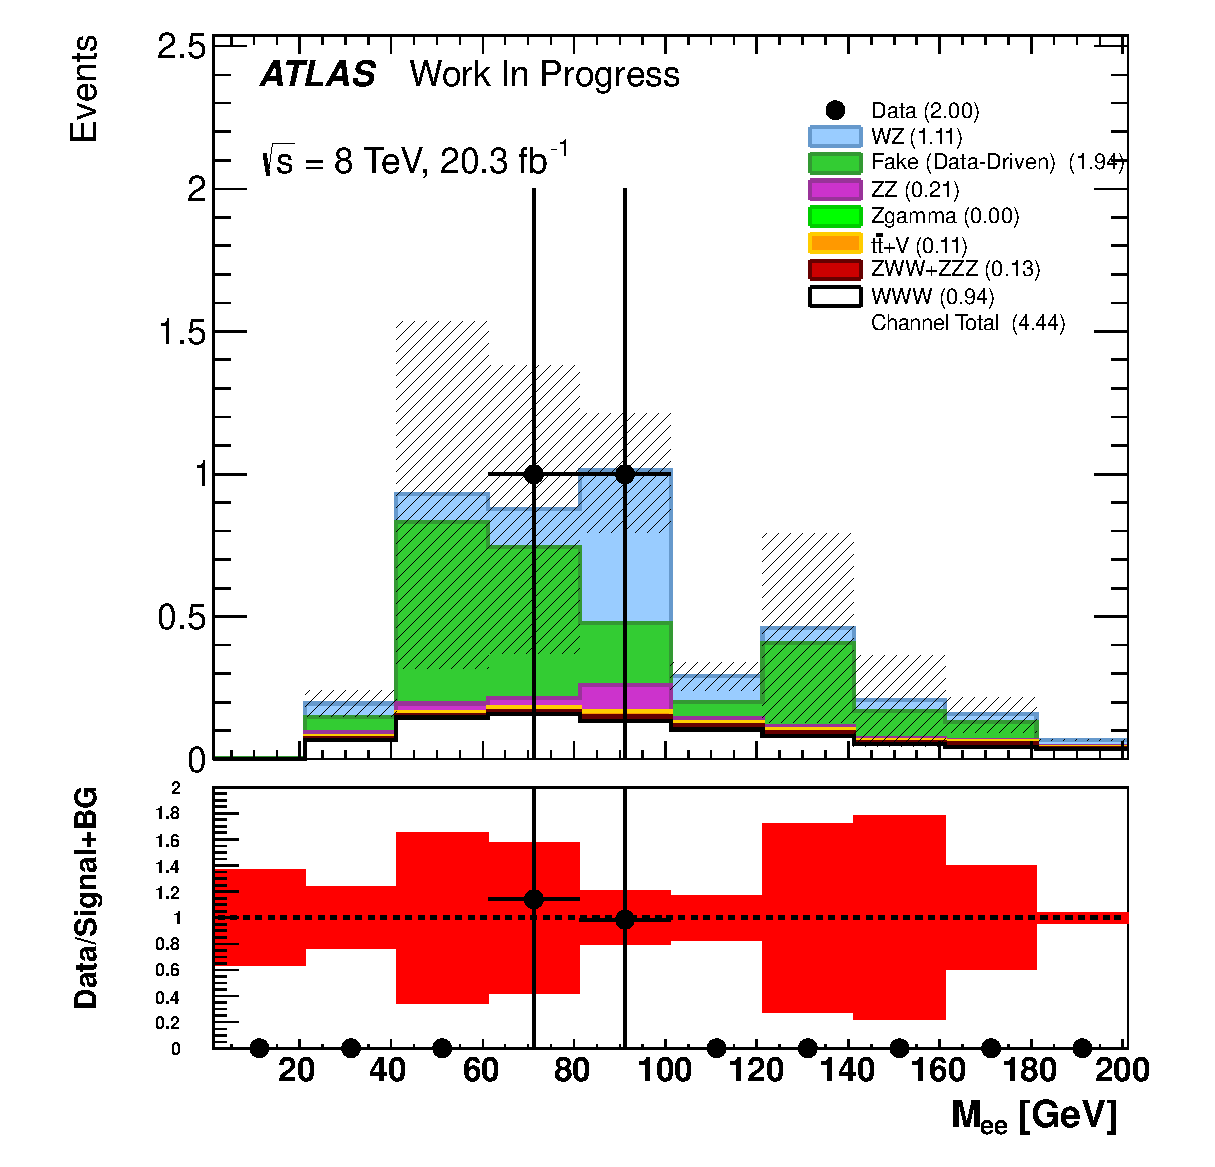
\includegraphics[width=0.3\columnwidth]{figures/appendix_signal_selection/Nov24Update_FakeSys_KFacSys_LinearY_Rebin/output/jobs/MxM/DataFull_Rates_May13_FakeRatesExactly2Loose_MuonMxMBJetGt0_ElBJetGt0SubtractPC_MxM/PreselectionNov23_15_0SFOS_ChargeAbs1_BVeto85_SFMllGt20_physics/weight_all/eps/InvariantMassElEl_histratio.eps}
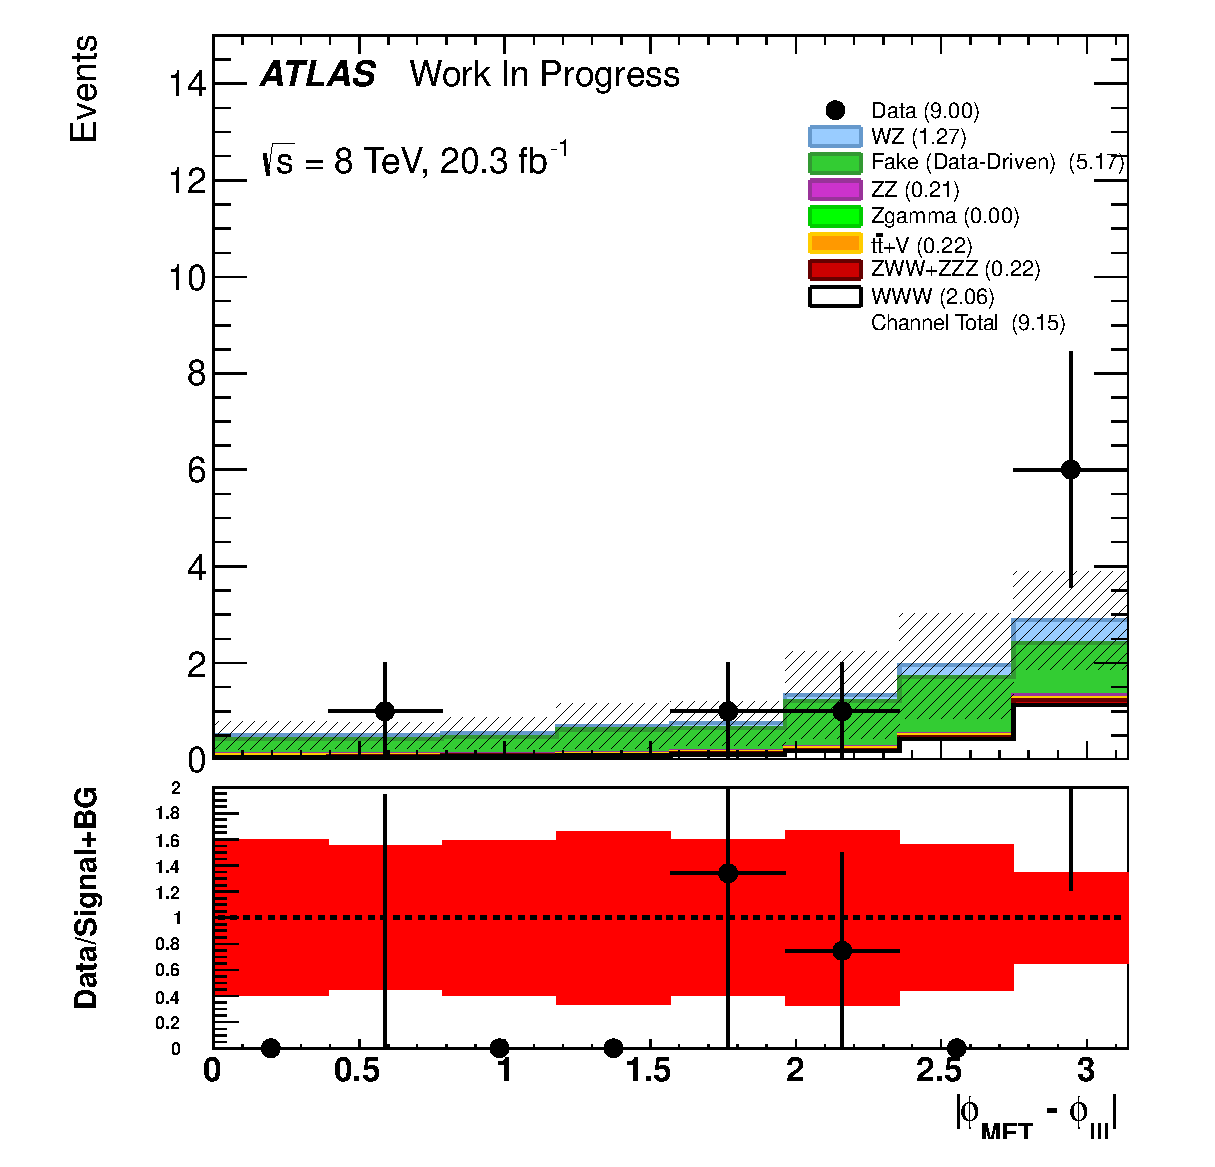
\includegraphics[width=0.3\columnwidth]{figures/appendix_signal_selection/Nov24Update_FakeSys_KFacSys_LinearY_Rebin/output/jobs/MxM/DataFull_Rates_May13_FakeRatesExactly2Loose_MuonMxMBJetGt0_ElBJetGt0SubtractPC_MxM/PreselectionNov23_15_0SFOS_ChargeAbs1_BVeto85_SFMllGt20_SSMeeZVeto15_physics/weight_all/eps/DeltaPhiMET123_Abs_histratio.eps}
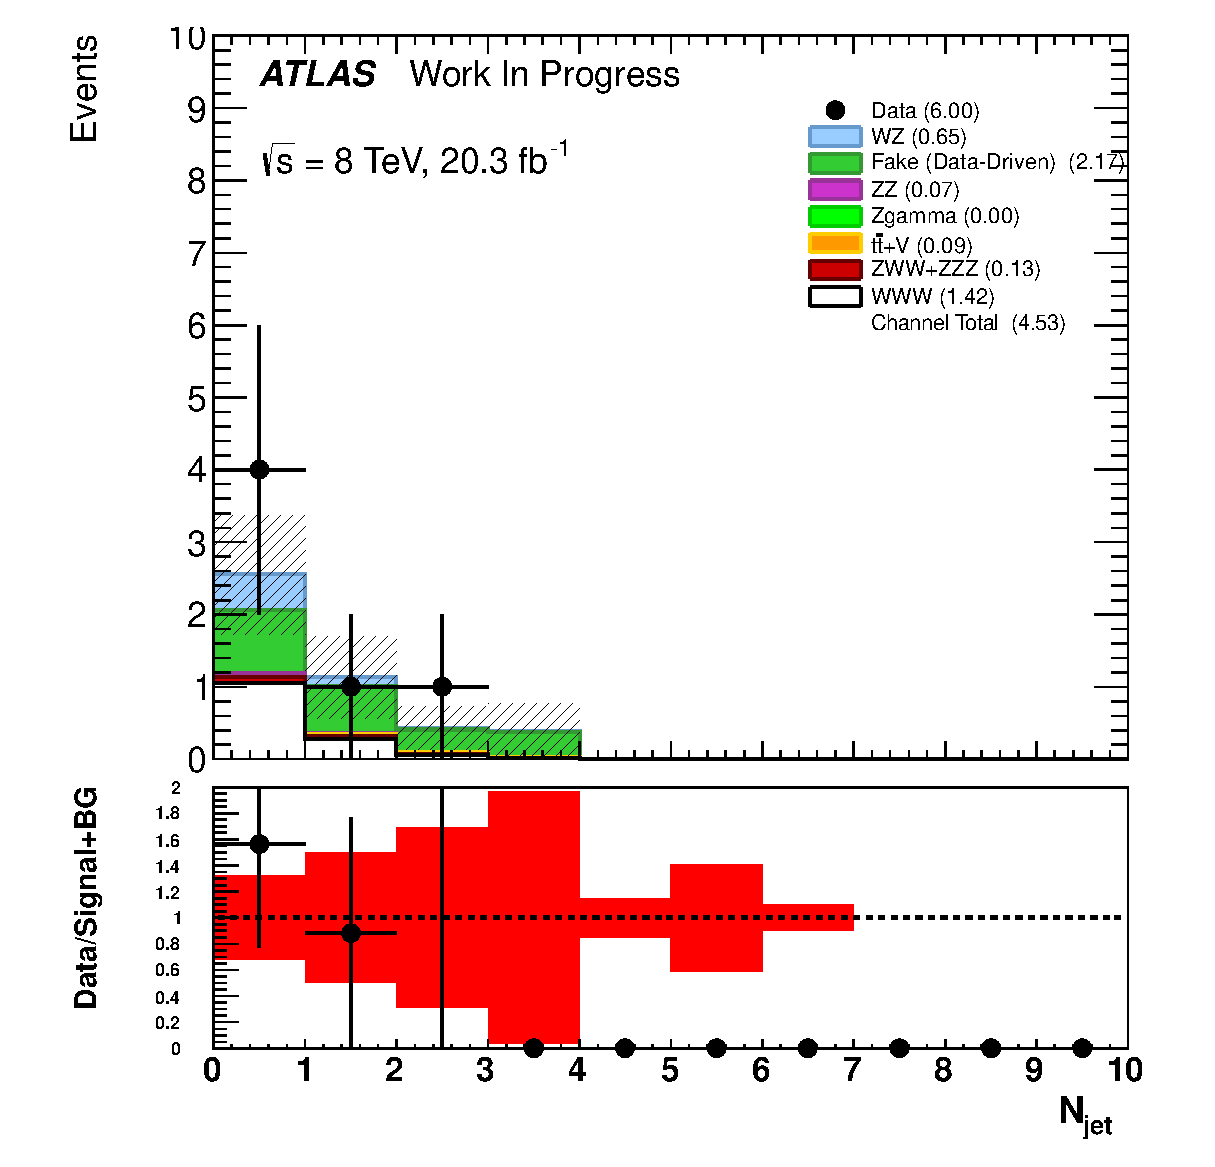
\includegraphics[width=0.3\columnwidth]{figures/appendix_signal_selection/Nov24Update_FakeSys_KFacSys_LinearY_Rebin/output/jobs/MxM/DataFull_Rates_May13_FakeRatesExactly2Loose_MuonMxMBJetGt0_ElBJetGt0SubtractPC_MxM/PreselectionNov23_15_0SFOS_ChargeAbs1_BVeto85_SFMllGt20_SSMeeZVeto15_DeltaPhi2p5_physics/weight_all/eps/NJets_histratio.eps}
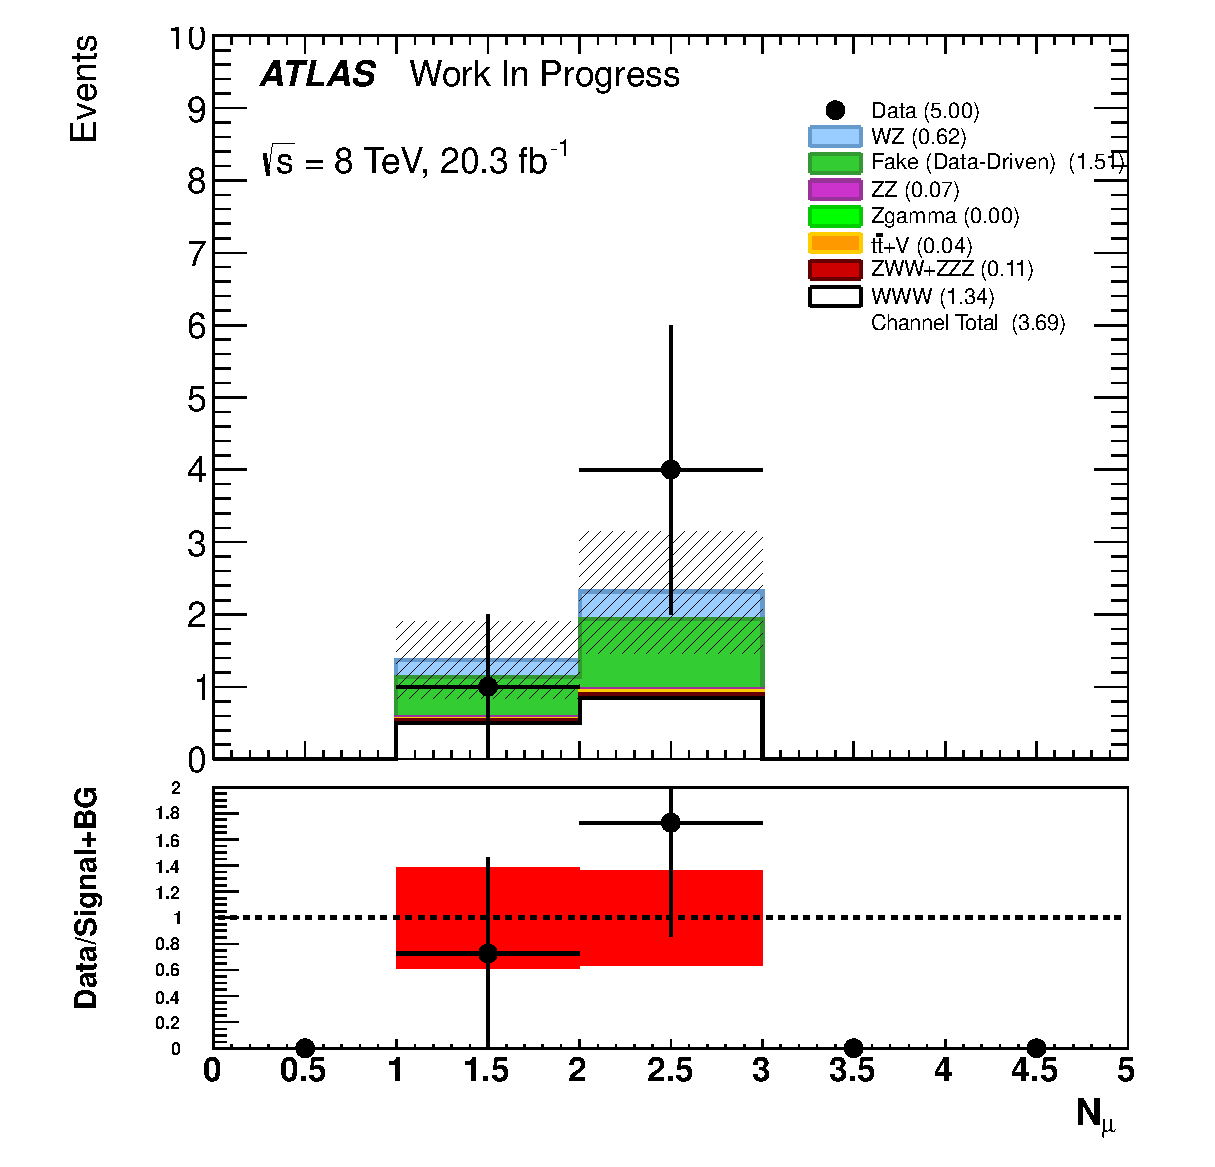
\includegraphics[width=0.3\columnwidth]{figures/appendix_signal_selection/Nov24Update_FakeSys_KFacSys_LinearY_Rebin/output/jobs/MxM/DataFull_Rates_May13_FakeRatesExactly2Loose_MuonMxMBJetGt0_ElBJetGt0SubtractPC_MxM/PreselectionNov23_15_0SFOS_ChargeAbs1_BVeto85_SFMllGt20_SSMeeZVeto15_DeltaPhi2p5_NJetLt2_physics/weight_all/eps/NMuons_histratio.eps}

%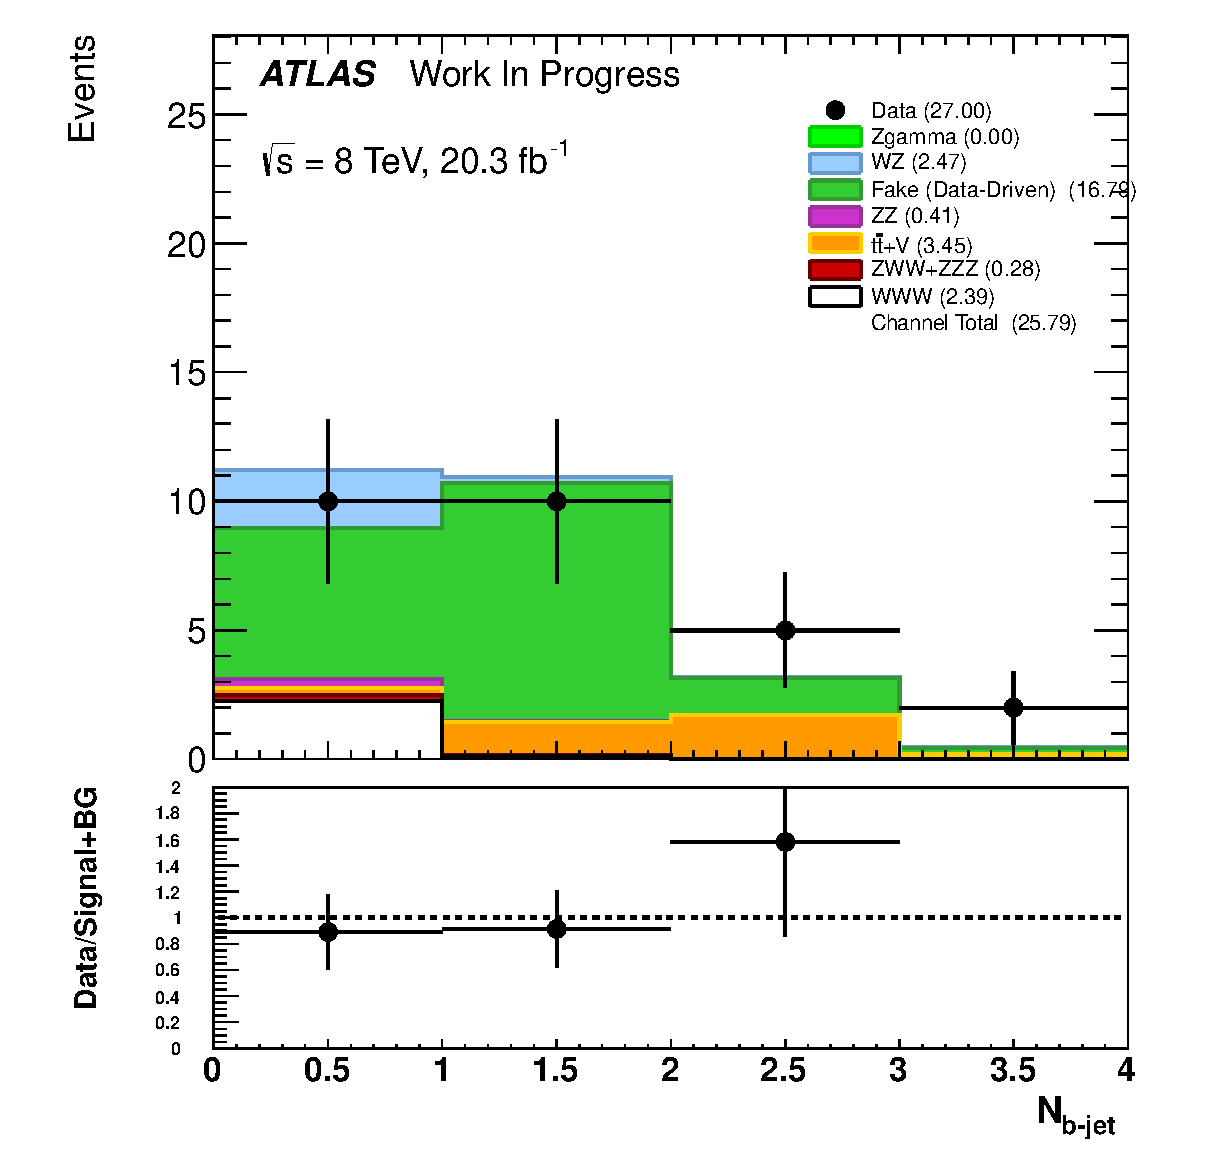
\includegraphics[width=0.3\columnwidth]{figures/appendix_signal_selection/PreselectionJune2_NoSTVF_0SFOS_ChargeAbs1_physics/weight_all/eps/NBTaggedJets_histratio.eps}
%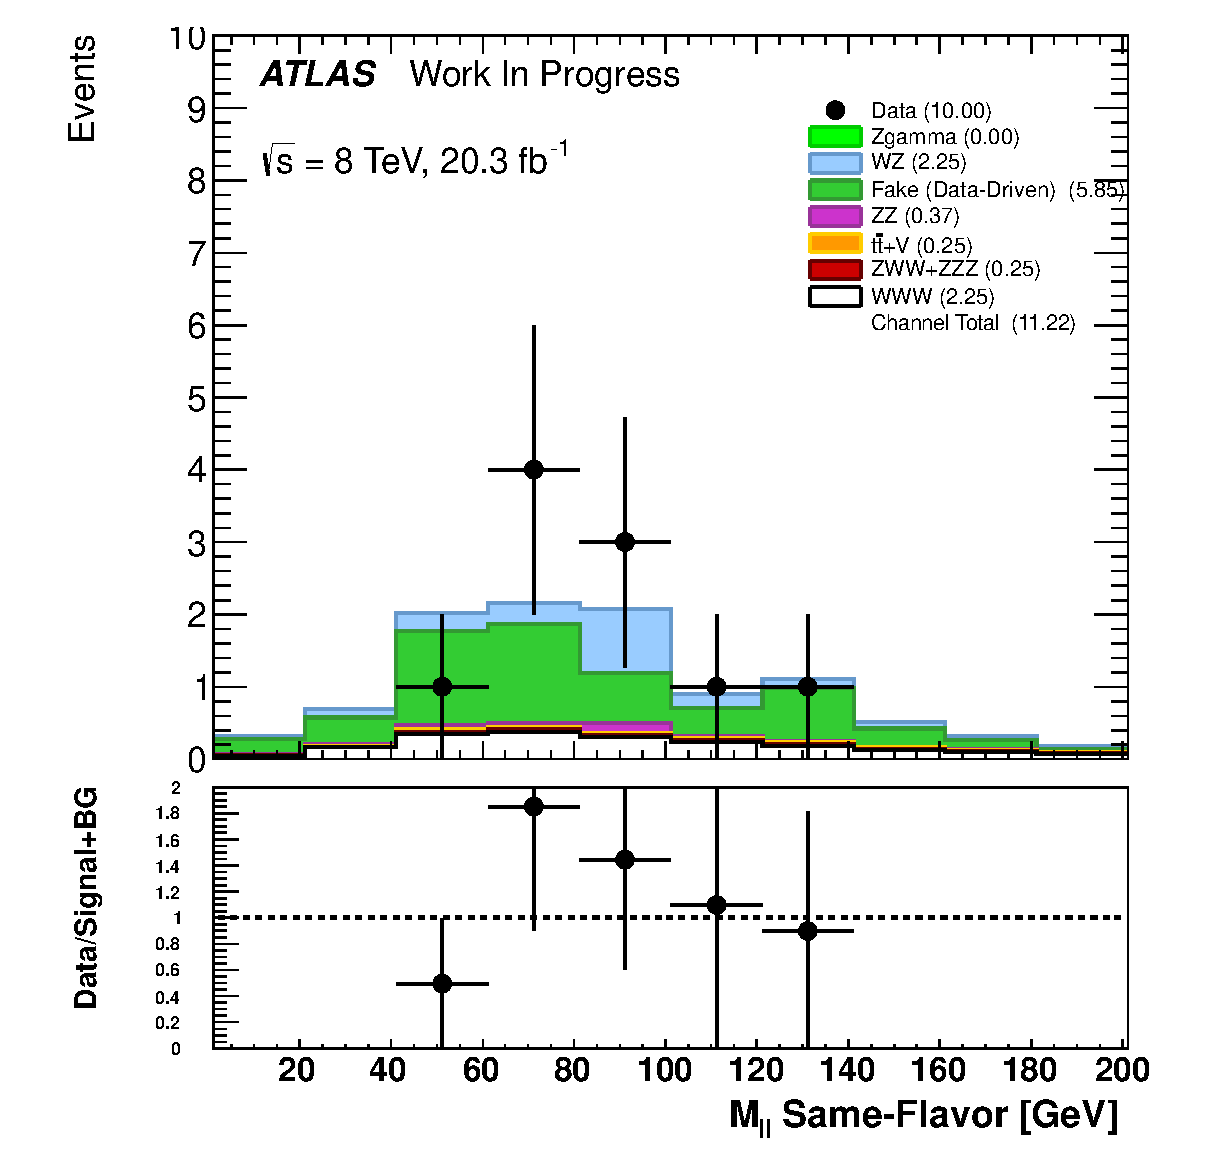
\includegraphics[width=0.3\columnwidth]{figures/appendix_signal_selection/PreselectionJune2_NoSTVF_0SFOS_ChargeAbs1_BVeto85_physics/weight_all/eps/InvariantMassSF_histratio.eps}
%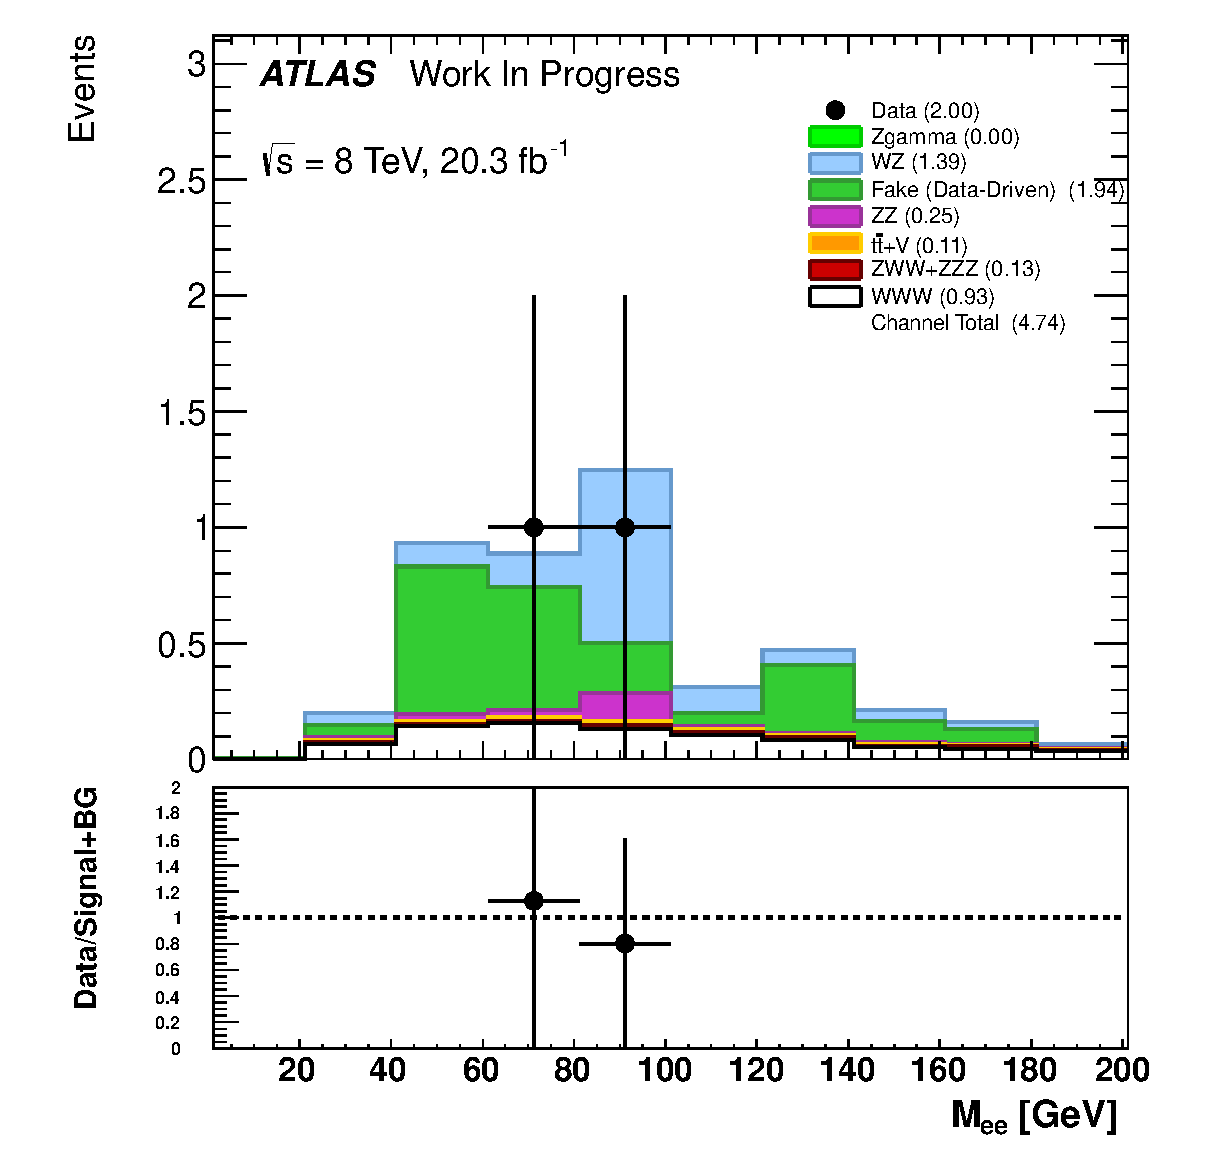
\includegraphics[width=0.3\columnwidth]{figures/appendix_signal_selection/PreselectionJune2_NoSTVF_0SFOS_ChargeAbs1_BVeto85_SFMllGt20_physics/weight_all/eps/InvariantMassElEl_histratio.eps}
%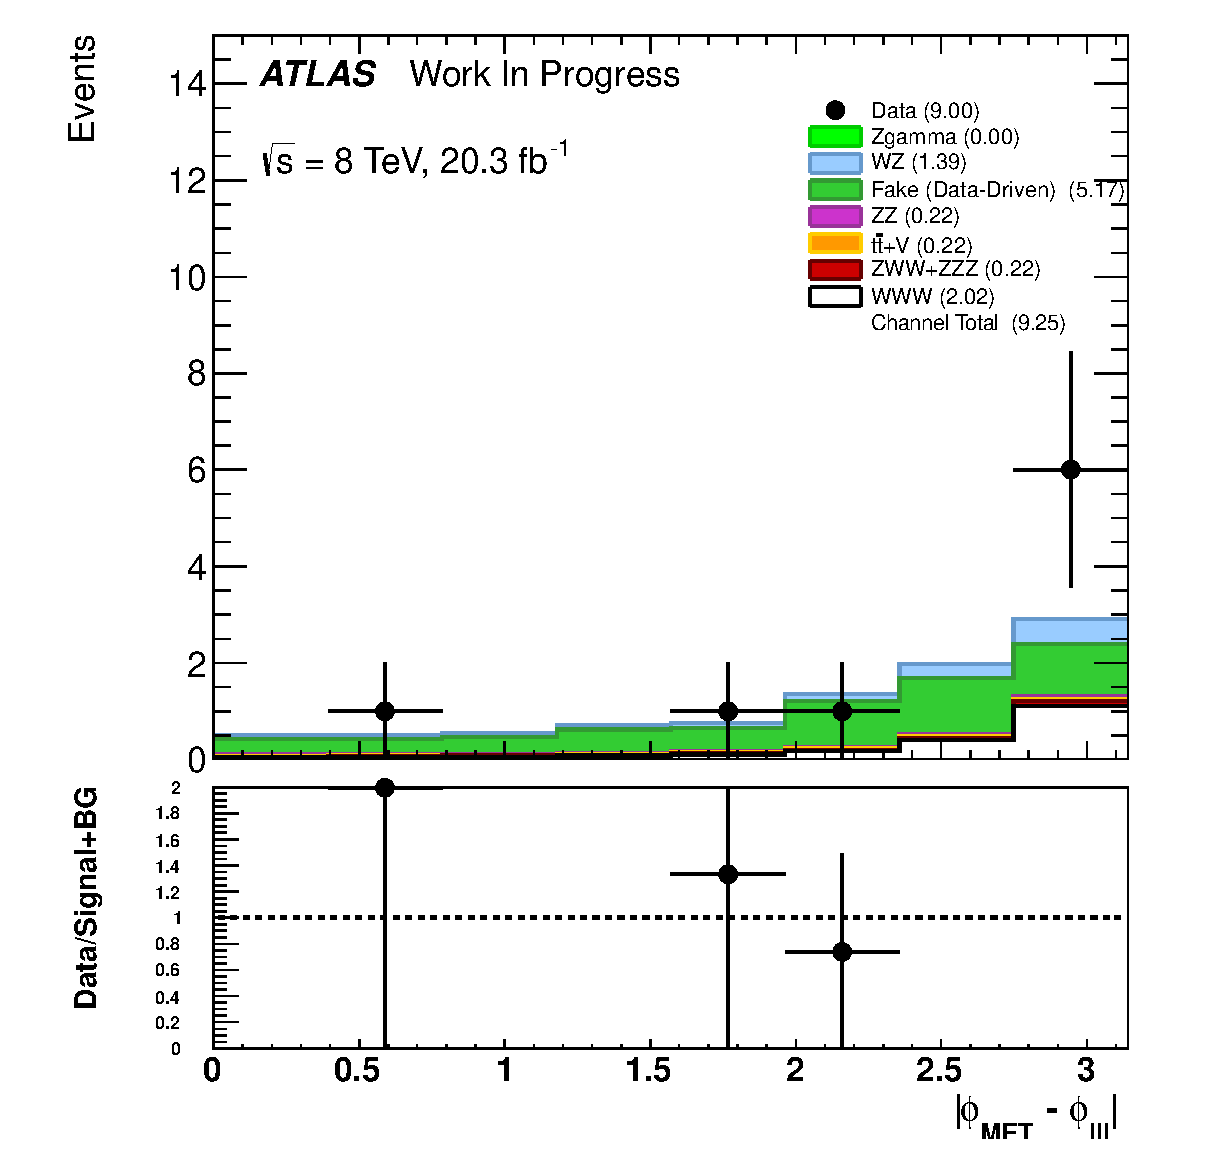
\includegraphics[width=0.3\columnwidth]{figures/appendix_signal_selection/PreselectionJune2_NoSTVF_0SFOS_ChargeAbs1_BVeto85_SFMllGt20_SSMeeZVeto15_physics/weight_all/eps/DeltaPhiMET123_Abs_histratio.eps}
%\includegraphics[width=0.3\columnwidth]{figures/appendix_signal_selection/PreselectionJune2_NoSTVF_0SFOS_ChargeAbs1_BVeto85_SFMllGt20_SSMeeZVeto15_DeltaPhi2p5_physics/weight_all/eps/NJets_histratio.eps}
%\includegraphics[width=0.3\columnwidth]{figures/appendix_signal_selection/PreselectionJune2_NoSTVF_0SFOS_ChargeAbs1_BVeto85_SFMllGt20_SSMeeZVeto15_DeltaPhi2p5_NJetLt2_physics/weight_all/eps/NMuons_histratio.eps}
\caption{Distributions showing data compared to the signal plus background estimate in the 0 SFOS region at each stage 
of the selection before the cuts are applied to the given distribution. 
Plots should be read sequentially from left to right
and from top to bottom. 
Referring to Table~\ref{tab:cutflow_weighted_0sfos}, the top left
plot is shown before cut \#3 is applied, top middle is before cut \#5, and
so on until the bottom right which is after all cuts are applied.
}
\label{fig:0sfos}
\end{figure}

The prediction from the 0 SFOS signal region at each stage of the selection
is summarized in 
\tab\ref{tab:cutflow_weighted_0sfos}
for the signal and background predictions, as well as for the data.
There is also a more detailed set of predictions at each stage for the 
different background sources in 
\tab\ref{tab:cutflow_weighted_0sfos_bg}. 
From this, we can clearly see the enormous impact of the 0 SFOS
cut on removing the backgrounds, for the $WZ$ background in particular.
We can also see the strong impact that the \nbjet~and \deltaphi~
cuts have without removing much of the signal.
We can also see the signal plus background predictions as 
compared to the data
for the distribution just before each cut is applied in 
\fig\ref{fig:0sfos}. From this we can clearly see
that the data seems to be well modeled at each stage of the selection.

After the full selection is applied,
the 0 SFOS signal region is found to be the most sensitive of the three
channels, as expected, with a predicted signal to background ratio of 56\%.
This can be seen from \tab\ref{tab:sys_summary}, where the expected signal
is 1.344 compared to an expected background of 2.35. Together they 
combine to give a total prediction of 3.69 signal plus background events. 
The Poisson probability of observing $\leq 5$ events with 3.69 events expected 
from the signal plus background prediction is 30.7\%. 
Thus, we can see that this is in good agreement with the observed 5 events in data
from the statistical uncertainty alone. 

The fake background makes up more than half of the total expected background
prediction, with 1.51 background events predicted from fakes compared to 
2.35 events expected from the total background.  The systematic
uncertainty on the fake background is approaching 100\%.
As can be seen in \tab\ref{tab:sys_breakdown}, this results in the
systematic uncertainty on the total background estimate 
that is approaching 60\%, or roughly the size of the fake
background contribution.
This further increases the compatibility 
of the data with the expectation, but also reduces the sensitivity.

The other backgrounds are less important. The $WZ$ background
is the second largest, coming from charge mis-identification, 
with $0.6176$ events predicted. The uncertainty on the $WZ$
background is dominated by that from the $WZ$ normalization uncertainty,
which is 10\%, and also has a small contribution from the 
charge mis-identification estimate uncertainty.
The $VVV$ contributions is the third largest, predicting 0.1126
with a small uncertainty.
The $ZZ$ background has a similar source and 
uncertainty as the $WZ$, but is about 10 times
smaller in size. The $\ttV$ background contributes even less
and the DPS and $Z\gamma$ backgrounds have
0 contribution within the statistical uncertainties of the MC.



\subsubsection{1 SFOS Signal Region}

\begin{table}[ht!]
\small
\centering
\begin{tabular}{l||c|c||c|c||c|c}
\hline
 &                 \multicolumn{2}{c||}{Signal}            &  \multicolumn{2}{c||}{Background} &  \multicolumn{2}{c}{Data} \\
   & Yield & Eff. & Yield & Eff. & Yield & Eff.\\
   \hline\hline
   %1. Pre-selection &  $9.78$ & --- &  $2388.48$ & --- & $2472$ &  --- \\
   %\hline
   1. 1 SFOS &  $4.67$ &  --- &  $1231.49$ &  --- & $1260$ &  --- \\ 
   \hline
   2. $N_{\mathrm{b-jet}} = 0$ &  $4.42$ &  $0.94$ &  $1086.66$ &  $0.88$ & $1095$ &  $0.87$\\ 
   \hline
   3. NOT $m_Z - 35~\mathrm{GeV} <$  &  \multirow{2}{*}{$2.76$} &  \multirow{2}{*}{$0.63$} &  \multirow{2}{*}{$97.96$} &  \multirow{2}{*}{$0.090$} & \multirow{2}{*}{$93$} &  \multirow{2}{*}{$0.08$}\\ 
    \hfill$ m_{\mathrm{SFOS}} < m_Z + 20~\mathrm{GeV}$  & & & & &  & \\
   \hline
   4. $E_{T}^{Miss} > 45$ GeV &  $1.91$ &  $0.69$ &  $29.83$ &  $0.30$ & $27$ &  $0.29$\\ 
   \hline
   5. $|\Delta\phi(3l,E_{T}^{Miss})| > 2.5$ &  $1.48$ &  $0.77$ &  $16.73$ &  $0.56$ & $16$ &  $0.59$\\ 
   \hline
   6. $N_{\mathrm{Jet}} \leq 1$ &  $1.39$ &  $0.94$ &  $14.77$ &  $0.88$ & $13$ &  $0.81$\\ 
   \hline
   \end{tabular}

\caption{Cut-flows showing the event yields and efficiencies for each cut in the 1 SFOS signal region
starting from event pre-selection separately for the total signal and total background predictions, along with the observed by data. 
Event yields for MC backgrounds and signal include all weights and are normalized to an integrated luminosity of $20.3~\mathrm{fb}^{-1}$.  
The fake lepton background only includes the matrix method weights.  The data is unweighted.
Efficiencies show the ratio of the yield with respect
to the previous cut.  The efficiency is first calculated at the first cut after event pre-selection.  }
\label{tab:cutflow_weighted_1sfos}
\end{table}

\begin{table}[ht!]
\small
\centering
\begin{tabular}{l||c|c||c|c||c|c}
\hline
 &       \multicolumn{6}{c}{Background}\\
 &  \multicolumn{2}{c||}{$WZ$} & \multicolumn{2}{c||}{$ZZ$} & \multicolumn{2}{c}{$t\bar{t}+V$} \\ 
 & Yield & Eff. & Yield & Eff. & Yield & Eff. \\
\hline\hline
Pre-selection & $1566.91$ & --- &  $323.60$ & --- &  $36.93$ & ---  \\
\hline
1. 1 SFOS &  $757.38$ &  $0.48$ &  $171.39$ &  $0.53$ &  $18.10$ &  $0.49$ \\ 
\hline
2. $N_{\mathrm{b-jet}} = 0$ &  $696.90$ &  $0.92$ &  $150.14$ &  $0.88$ &  $1.42$ &  $0.08$\\ 
\hline
3. NOT $m_Z - 35~\mathrm{GeV} <$  &  \multirow{2}{*}{$44.30$} &  \multirow{2}{*}{$0.06$} &  \multirow{2}{*}{$13.79$} &  \multirow{2}{*}{$0.09$} &  \multirow{2}{*}{$0.37$} &  \multirow{2}{*}{$0.26$} \\ 
\hfill $ m_{\mathrm{SFOS}} < m_Z + 20~\mathrm{GeV}$ & & & &  & & \\
\hline
4. $E_{T}^{Miss} > 45$ GeV &  $21.38$ &  $0.48$ &  $1.46$ &  $0.11$ &  $0.29$ &  $0.78$ \\ 
\hline
5. $|\Delta\phi(3l,E_{T}^{Miss})| > 2.5$ &  $13.07$ &  $0.61$ &  $0.71$ &  $0.49$ &  $0.11$ &  $0.39$ \\ 
\hline
6. $N_{\mathrm{Jet}} \leq 1$ &  $11.90$ &  $0.91$ &  $0.58$ &  $0.82$ &  $0.05$ &  $0.45$ \\ 
\hline
\end{tabular}

\begin{tabular}{l||c|c||c|c||c|c}
\hline
 &       \multicolumn{6}{c}{Background}\\
 &  \multicolumn{2}{c||}{$ZZZ+ZWW$} & \multicolumn{2}{c||}{$Z\gamma$} & \multicolumn{2}{c}{Fake} \\ 
 & Yield & Eff. & Yield & Eff. & Yield & Eff. \\
\hline\hline
%1. Pre-selection &  $3.12$ & --- &  $219.80$ & --- &  $238.12$ & ---  \\
%\hline
1 SFOS &  $1.55$ &  --- &  $149.60$ &  --- &  $133.47$ &  --- \\ 
\hline
$N_{\mathrm{b-jet}} = 0$ &  $1.31$ &  $0.84$ &  $136.96$ &  $0.92$ &  $99.93$ &  $0.75$ \\ 
\hline
NOT $m_Z - 35~\mathrm{GeV} <$  &  \multirow{2}{*}{$0.34$} &  \multirow{2}{*}{$0.26$} &  \multirow{2}{*}{$22.44$} &  \multirow{2}{*}{$0.16$} &  \multirow{2}{*}{$16.72$} &  \multirow{2}{*}{$0.17$} \\ 
$ m_{\mathrm{SFOS}} < m_Z + 20~\mathrm{GeV}$ & & & & & &  \\
\hline
$E_{T}^{Miss} > 45$ GeV &  $0.24$ &  $0.71$ &  $1.36$ &  $0.06$ &  $5.10$ &  $0.31$ \\ 
\hline
$|\Delta\phi(3l,E_{T}^{Miss})| > 2.5$ &  $0.17$ &  $0.69$ &  $0.20$ &  $0.15$ &  $2.47$ &  $0.48$ \\ 
\hline
$N_{\mathrm{Jet}} \leq 1$ &  $0.14$ &  $0.84$ &  $0.20$ &  $1.00$ &  $1.90$ &  $0.77$\\ 
\hline
\end{tabular}

\caption{Cut-flows showing the event yields and efficiencies for each cut in the 1 SFOS signal region
starting from event pre-selection and binned by background category. 
Event yields for MC backgrounds and signal include all weights and are normalized to an integrated luminosity of $20.3~\mathrm{fb}^{-1}$.  
The fake lepton background only includes the matrix method weights.  The data is unweighted.
Efficiencies show the ratio of the yield with respect
to the previous cut.  The efficiency is first calculated at the first cut after event pre-selection.  }
\label{tab:cutflow_weighted_1sfos_bg}
\end{table}


%1 SFOS consolidated
\begin{figure}[ht!]
\centering
\includegraphics[width=0.3\columnwidth]{figures/appendix_signal_selection/Nov24Update_FakeSys_KFacSys_LinearY_Rebin/output/jobs/MxM/DataFull_Rates_May13_FakeRatesExactly2Loose_MuonMxMBJetGt0_ElBJetGt0SubtractPC_MxM/PreselectionNov23_15_1SFOS_ChargeAbs1_physics/weight_all/eps/NBTaggedJets_histratio.eps}
\includegraphics[width=0.3\columnwidth]{figures/appendix_signal_selection/Nov24Update_FakeSys_KFacSys_LinearY_Rebin/output/jobs/MxM/DataFull_Rates_May13_FakeRatesExactly2Loose_MuonMxMBJetGt0_ElBJetGt0SubtractPC_MxM/PreselectionNov23_15_1SFOS_ChargeAbs1_BVeto85_physics/weight_all/eps/InvariantMassSFOS_histratio.eps}
\includegraphics[width=0.3\columnwidth]{figures/appendix_signal_selection/Nov24Update_FakeSys_KFacSys_LinearY_Rebin/output/jobs/MxM/DataFull_Rates_May13_FakeRatesExactly2Loose_MuonMxMBJetGt0_ElBJetGt0SubtractPC_MxM/PreselectionNov23_15_1SFOS_ChargeAbs1_BVeto85_ZVetoLow35High25GeV_physics/weight_all/eps/MET_Et_histratio.eps}
\includegraphics[width=0.3\columnwidth]{figures/appendix_signal_selection/Nov24Update_FakeSys_KFacSys_LinearY_Rebin/output/jobs/MxM/DataFull_Rates_May13_FakeRatesExactly2Loose_MuonMxMBJetGt0_ElBJetGt0SubtractPC_MxM/PreselectionNov23_15_1SFOS_ChargeAbs1_BVeto85_ZVetoLow35High25GeV_METGt45GeV_physics/weight_all/eps/DeltaPhiMET123_Abs_histratio.eps}
\includegraphics[width=0.3\columnwidth]{figures/appendix_signal_selection/Nov24Update_FakeSys_KFacSys_LinearY_Rebin/output/jobs/MxM/DataFull_Rates_May13_FakeRatesExactly2Loose_MuonMxMBJetGt0_ElBJetGt0SubtractPC_MxM/PreselectionNov23_15_1SFOS_ChargeAbs1_BVeto85_ZVetoLow35High25GeV_METGt45GeV_DeltaPhi2p5_physics/weight_all/eps/NJets_histratio.eps}
\includegraphics[width=0.3\columnwidth]{figures/appendix_signal_selection/Nov24Update_FakeSys_KFacSys_LinearY_Rebin/output/jobs/MxM/DataFull_Rates_May13_FakeRatesExactly2Loose_MuonMxMBJetGt0_ElBJetGt0SubtractPC_MxM/PreselectionNov23_15_1SFOS_ChargeAbs1_BVeto85_ZVetoLow35High25GeV_METGt45GeV_DeltaPhi2p5_NJetLt2_physics/weight_all/eps/NMuons_histratio.eps}


%\includegraphics[width=0.3\columnwidth]{figures/appendix_signal_selection/PreselectionMay29_1SFOS_ChargeAbs1_physics/weight_all/eps/NBTaggedJets_histratio.eps}
%\includegraphics[width=0.3\columnwidth]{figures/appendix_signal_selection/PreselectionMay29_1SFOS_ChargeAbs1_BVeto85_physics/weight_all/eps/InvariantMassSFOS_histratio.eps}
%\includegraphics[width=0.3\columnwidth]{figures/appendix_signal_selection/PreselectionMay29_1SFOS_ChargeAbs1_ZVetoLow35High25GeV_physics/weight_all/eps/MET_Et_histratio.eps}
%\includegraphics[width=0.3\columnwidth]{figures/appendix_signal_selection/PreselectionJune2_NoSTVF_1SFOS_ChargeAbs1_ZVetoLow35High25GeV_BVeto85_METGt45GeV_physics/weight_all/eps/DeltaPhiMET123_Abs_histratio.eps}
%\includegraphics[width=0.3\columnwidth]{figures/appendix_signal_selection/PreselectionJune2_NoSTVF_1SFOS_ChargeAbs1_ZVetoLow35High25GeV_BVeto85_METGt45GeV_DeltaPhi2p5_physics/weight_all/eps/NJets_histratio.eps}
%\includegraphics[width=0.3\columnwidth]{figures/appendix_signal_selection/PreselectionJune2_NoSTVF_1SFOS_ChargeAbs1_ZVetoLow35High25GeV_BVeto85_METGt45GeV_DeltaPhi2p5_NJetLt2_physics/weight_all/eps/NMuons_histratio.eps}
\caption{Distributions showing data compared to the signal plus background estimate in the 1 SFOS region at each stage 
of the selection before the cuts are applied to the given distribution. Plots should be read sequentially from left to right
and from top to bottom. 
Referring to Table~\ref{tab:cutflow_weighted_1sfos}, the top left
plot is shown before cut \#3 is applied, top middle is before cut \#4, and
so on until the bottom right which is after all cuts are applied.}
\label{fig:1sfos}
\end{figure}



The 1 SFOS signal region is not as sensitive as the 0 SFOS region, with 
a signal to background ratio of about 9.2\%.
The background is overwhelmingly dominated by $WZ$ contributions. 
Similar to the 0 SFOS region, the predictions and data
at each stage of the 1 SFOS signal region selection are shown in
\tab\ref{tab:cutflow_weighted_1sfos}
and 
\tab\ref{tab:cutflow_weighted_1sfos_bg}. 
The 1 SFOS requirement leaves much of the $WZ$ and $ZZ$ backgrounds,
but the \z-veto and \MET~cuts
are very effective at removing most of this while keeping the signal.


Again, we can also see the signal plus background predictions as 
compared to the data
for the distribution just before each cut is applied in 
the 1 SFOS region by looking at \fig\ref{fig:1sfos}. 
Here, the distributions again appear to be well modeled
at each stage of the selection.  Looking closer
at the \njet~distribution, we can see that there is a deficit
of data in the $\njet=1$ bin which is kept in the seleciton
and results in a slight deficit in the prediction. 
Further, if we look at the \nmu~distibution we see that
this deficit seems to fall exclusively in the $\nmu=1$ bin.
A more detailed investigation of the cutflows
in the individual $\nmu=1$ and $\nmu=2$ bins suggests that 
this is most likely a statisitcal fluctuation.
Overall, the deficit is not very significant, with the Poisson
probability of observing 13 or less events with 16.16 expected
being 26.2\%.


The fake background is only the second largest background in 
this region, making up about 13\% of the total. Still, even with 
the 10\% uncertainty on the normalization of the dominant $WZ$
background, the fake background uncertainty is the largest
uncertainty on the background estimation, approaching 13\%, as
can be seen in \tab\ref{tab:sys_breakdown}.
The \ttV~ and $VVV$ backgrounds are of a similar absolute size as in
the 0 SFOS region, but the larger overall background makes them
even less important. The DPS and $Z\gamma$ uncertainties
contribute a finite amount to the background within the statistical
uncertainties, but remain negligible.

%\begin{table}[ht!]
%\centering
%\begin{tabular}{|c||c|c|c|c|}
\hline
 & $eee$ & $ee\mu$ & $e\mu\mu$ & $\mu\mu\mu$\\ 
\hline\hline
$WZ$ &  $0.0 \pm 0$ &  $5.321 \pm 0.099$ &  $6.58 \pm 0.11$ &  $0.0 \pm 0$\\ 
$ZZ$ &  $0.0 \pm 0$ &  $0.324 \pm 0.012$ &  $0.259 \pm 0.011$ &  $0.0 \pm 0$\\ 
$Z\gamma$ &  $0.0 \pm 0$ &  $0.0 \pm 0$ &  $0.20 \pm 0.13$ &  $0.0 \pm 0$\\ 
$ZWW+ZZZ$ &  $0.0 \pm 0$ &  $0.0660 \pm 0.0077$ &  $0.074 \pm 0.008$ &  $0.0 \pm 0$\\ 
$t\bar{t}+V$ &  $0.0 \pm 0$ &  $0.0207 \pm 0.0031$ &  $0.0296 \pm 0.0036$ &  $0.0 \pm 0$\\ 
Fake (data-driven) &  $0.0 \pm 0$ &  $0.71 \pm 0.18$ &  $1.19 \pm 0.29$ &  $0.0 \pm 0$\\ 
$WWW$ &  $0.0 \pm 0$ &  $0.61 \pm 0.01$ &  $0.760 \pm 0.012$ &  $0.0 \pm 0$\\ 
\hline
Expected Background &  $0.0 \pm 0$ &  $6.44 \pm 0.21$ &  $8.33 \pm 0.34$ &  $0.0 \pm 0$\\ 
Expected Signal + Background &  $0.0 \pm 0$ &  $7.05 \pm 0.21$ &  $9.09 \pm 0.34$ &  $0.0 \pm 0$\\ 
\hline
Observed Data &  $0.0 \pm 0$ &  $2.0 \pm 1.4$ &  $11.0 \pm 3.3$ &  $0.0 \pm 0$\\ 
\hline
\end{tabular}

%\caption{ Expected and observed event yields binned by lepton flavor combination for the optimized 1 SFOS signal region selection defined as follows: event pre-selection + 1 SFOS + b-veto + Z-veto + $\Delta\phi$ + $N_{jet}$ requirements.
%Only statistical uncertainties are shown.
%}
%\label{tab:1sfos}
%\end{table}

\subsubsection{2 SFOS Signal Region}

\begin{table}[ht!]
\small
\centering
%\scriptsize
\begin{tabular}{l||c|c||c|c||c|c}
\hline
 &                 \multicolumn{2}{c||}{Signal}            &  \multicolumn{2}{c||}{Background} &  \multicolumn{2}{c}{Data} \\
   & Yield & Eff. & Yield & Eff. & Yield & Eff.\\
   \hline\hline
   %1. Pre-selection &  $9.78$ & --- &  $2388.48$ & --- & $2472$ &  --- \\ 
   %\hline
   1. 2 SFOS &  $2.66$ &  --- &  $1132.53$ &  --- & $1182$ & ---\\ 
   \hline
   2. $N_{\mathrm{b-jet}}=0$ &  $2.50$ &  $0.94$ &  $1012.07$ &  $0.89$ & $1033$ &  $0.87$\\ 
   \hline
   3. $| m_{\mathrm{SFOS}} - m_Z | >  20$ GeV &  $1.46$ &  $0.58$ &  $108.88$ &  $0.11$ & $108$ &  $0.10$\\ 
   \hline
   4. $E_{T}^{Miss} > 55$ GeV &  $0.83$ &  $0.57$ &  $18.99$ &  $0.17$ & $18$ &  $0.17$\\ 
   \hline
   5. $|\Delta\phi(3l,E_{T}^{Miss})| > 2.5$ &  $0.65$ &  $0.78$ &  $11.64$ &  $0.61$ & $8$ &  $0.44$\\ 
   \hline
   6. $N_{\mathrm{Jet}} \leq 1$ &  $0.61$ &  $0.94$ &  $10.25$ &  $0.88$ & $6$ &  $0.75$\\ 
   \hline
   \end{tabular}



\caption{Cut-flows showing the event yields and efficiencies for each cut in the 2 SFOS signal region
starting from event pre-selection separately for the total signal and total background predictions, along with the observed data.
Event yields for MC backgrounds and signal include all weights and are normalized to an integrated luminosity of $20.3~\mathrm{fb}^{-1}$.  
The fake lepton background only includes the matrix method weights.  The data is unweighted.
Efficiencies show the ratio of the yield with respect
to the previous cut.  The efficiency is first calculated at the first cut after event pre-selection.  }
\label{tab:cutflow_weighted_2sfos}
\end{table}

\begin{table}[ht!]
\small
\centering
%\scriptsize
\begin{tabular}{l||c|c||c|c||c|c}
\hline
 &       \multicolumn{6}{c}{Background} \\
 & \multicolumn{2}{c||}{$WZ$} & \multicolumn{2}{c||}{$ZZ$} & \multicolumn{2}{c}{$t\bar{t}+V$}  \\ 
 & Yield & Eff. & Yield & Eff. & Yield & Eff.  \\
\hline\hline
Pre-selection &  $1566.91$ & --- &  $323.60$ & --- &  $36.93$ & --- \\ 
\hline
2 SFOS &  $807.27$ &  $0.52$ &  $151.28$ &  $0.47$ &  $15.35$ &  $0.42$  \\ 
\hline
$N_{\mathrm{b-jet}}=0$ &  $743.12$ &  $0.92$ &  $136.16$ &  $0.90$ &  $1.19$ &  $0.08$ \\ 
\hline
$| m_{\mathrm{SFOS}} - m_Z | >  20$ GeV &  $44.95$ &  $0.06$ &  $21.13$ &  $0.16$ &  $0.22$ &  $0.18$\\ 
\hline
$E_{T}^{Miss} > 55$ GeV &  $15.86$ &  $0.35$ &  $0.97$ &  $0.05$ &  $0.14$ &  $0.65$ \\ 
\hline
$|\Delta\phi(3l,E_{T}^{Miss})| > 2.5$ &  $10.09$ &  $0.64$ &  $0.55$ &  $0.57$ &  $0.07$ &  $0.49$ \\ 
\hline
$N_{\mathrm{Jet}} \leq 1$ &  $9.07$ &  $0.90$ &  $0.48$ &  $0.86$ &  $0.02$ &  $0.35$ \\ 
\hline
\end{tabular}


\begin{tabular}{l||c|c||c|c||c|c}
\hline
 &       \multicolumn{6}{c}{Background} \\
 & \multicolumn{2}{c||}{$ZZZ+ZWW$} & \multicolumn{2}{c||}{$Z\gamma$} & \multicolumn{2}{c}{Fake} \\ 
 & Yield & Eff. & Yield & Eff. & Yield & Eff. \\
\hline\hline
Pre-selection & $3.12$ & --- &  $219.80$ & --- &  $238.12$ & ---  \\ 
\hline
1. 2 SFOS &  $1.30$ &  $0.41$ &  $69.99$ &  $0.32$ &  $87.34$ &  $0.37$ \\ 
\hline
2. $N_{\mathrm{b-jet}}=0$ &  $1.10$ &  $0.85$ &  $64.70$ &  $0.92$ &  $65.80$ &  $0.75$ \\ 
\hline
3. $| m_{\mathrm{SFOS}} - m_Z | >  20$ GeV &  $0.19$ &  $0.17$ &  $29.52$ &  $0.46$ &  $12.87$ &  $0.20$ \\ 
\hline
4. $E_{T}^{Miss} > 55$ GeV &  $0.12$ &  $0.63$ &  $0.43$ &  $0.01$ &  $1.47$ &  $0.11$ \\ 
\hline
5. $|\Delta\phi(3l,E_{T}^{Miss})| > 2.5$ &  $0.10$ &  $0.82$ &  $0.11$ &  $0.25$ &  $0.72$ &  $0.49$ \\ 
\hline
6. $N_{\mathrm{Jet}} \leq 1$ &  $0.08$ &  $0.82$ &  $0.11$ &  $1.00$ &  $0.49$ &  $0.69$ \\ 
\hline
\end{tabular}


\caption{Cut-flows showing the event yields and efficiencies for each cut in the 2 SFOS signal region
starting from event pre-selection and binned by background category. 
Event yields for MC backgrounds and signal include all weights and are normalized to an integrated luminosity of $20.3~\mathrm{fb}^{-1}$.  
The fake lepton background only includes the matrix method weights.  The data is unweighted.
Efficiencies show the ratio of the yield with respect
to the previous cut.  The efficiency is first calculated at the first cut after event pre-selection.  }
\label{tab:cutflow_weighted_2sfos_bg}
\end{table}


%2 SFOS consolidated
\begin{figure}[ht!]
\centering
\includegraphics[width=0.3\columnwidth]{figures/appendix_signal_selection/Nov24Update_FakeSys_KFacSys_LinearY_Rebin/output/jobs/MxM/DataFull_Rates_May13_FakeRatesExactly2Loose_MuonMxMBJetGt0_ElBJetGt0SubtractPC_MxM/PreselectionNov23_15_2SFOS_ChargeAbs1_physics/weight_all/eps/NBTaggedJets_histratio.eps}
\includegraphics[width=0.3\columnwidth]{figures/appendix_signal_selection/Nov24Update_FakeSys_KFacSys_LinearY_Rebin/output/jobs/MxM/DataFull_Rates_May13_FakeRatesExactly2Loose_MuonMxMBJetGt0_ElBJetGt0SubtractPC_MxM/PreselectionNov23_15_2SFOS_ChargeAbs1_BVeto85_physics/weight_all/eps/InvariantMassSFOS_histratio.eps}
\includegraphics[width=0.3\columnwidth]{figures/appendix_signal_selection/Nov24Update_FakeSys_KFacSys_LinearY_Rebin/output/jobs/MxM/DataFull_Rates_May13_FakeRatesExactly2Loose_MuonMxMBJetGt0_ElBJetGt0SubtractPC_MxM/PreselectionNov23_15_2SFOS_ChargeAbs1_BVeto85_ZVeto20GeV_physics/weight_all/eps/MET_Et_histratio.eps}
\includegraphics[width=0.3\columnwidth]{figures/appendix_signal_selection/Nov24Update_FakeSys_KFacSys_LinearY_Rebin/output/jobs/MxM/DataFull_Rates_May13_FakeRatesExactly2Loose_MuonMxMBJetGt0_ElBJetGt0SubtractPC_MxM/PreselectionNov23_15_2SFOS_ChargeAbs1_BVeto85_ZVeto20GeV_METGt55GeV_physics/weight_all/eps/DeltaPhiMET123_Abs_histratio.eps}
\includegraphics[width=0.3\columnwidth]{figures/appendix_signal_selection/Nov24Update_FakeSys_KFacSys_LinearY_Rebin/output/jobs/MxM/DataFull_Rates_May13_FakeRatesExactly2Loose_MuonMxMBJetGt0_ElBJetGt0SubtractPC_MxM/PreselectionNov23_15_2SFOS_ChargeAbs1_BVeto85_ZVeto20GeV_METGt55GeV_DeltaPhi2p5_physics/weight_all/eps/NJets_histratio.eps}
\includegraphics[width=0.3\columnwidth]{figures/appendix_signal_selection/Nov24Update_FakeSys_KFacSys_LinearY_Rebin/output/jobs/MxM/DataFull_Rates_May13_FakeRatesExactly2Loose_MuonMxMBJetGt0_ElBJetGt0SubtractPC_MxM/PreselectionNov23_15_2SFOS_ChargeAbs1_BVeto85_ZVeto20GeV_METGt55GeV_DeltaPhi2p5_NJetLt2_physics/weight_all/eps/NMuons_histratio.eps}



%\includegraphics[width=0.3\columnwidth]{figures/appendix_signal_selection/PreselectionMay29_2SFOS_ChargeAbs1_physics/weight_all/eps/NBTaggedJets_histratio.eps}
%\includegraphics[width=0.3\columnwidth]{figures/appendix_signal_selection/PreselectionMay29_2SFOS_ChargeAbs1_BVeto85_physics/weight_all/eps/InvariantMassSFOS_histratio.eps}
%\includegraphics[width=0.3\columnwidth]{figures/appendix_signal_selection/PreselectionMay29_2SFOS_ChargeAbs1_BVeto85_ZVeto20GeV_physics/weight_all/eps/MET_Et_histratio.eps}
%\includegraphics[width=0.3\columnwidth]{figures/appendix_signal_selection/PreselectionJune2_NoSTVF_2SFOS_ChargeAbs1_BVeto85_ZVeto20GeV_METGt55GeV_physics/weight_all/eps/DeltaPhiMET123_Abs_histratio.eps}
%\includegraphics[width=0.3\columnwidth]{figures/appendix_signal_selection/PreselectionJune2_NoSTVF_2SFOS_ChargeAbs1_BVeto85_ZVeto20GeV_METGt55GeV_DeltaPhi2p5_physics/weight_all/eps/NJets_histratio.eps}
%\includegraphics[width=0.3\columnwidth]{figures/appendix_signal_selection/PreselectionJune2_NoSTVF_2SFOS_ChargeAbs1_BVeto85_ZVeto20GeV_METGt55GeV_DeltaPhi2p5_NJetLt2_physics/weight_all/eps/NMuons_histratio.eps}
\caption{Distributions showing data compared to the signal plus background estimate in the 2 SFOS region at each stage 
of the selection before the cuts are applied to the given distribution. Plots should be read sequentially from left to right
and from top to bottom. 
Referring to Table~\ref{tab:cutflow_weighted_2sfos}, the top left
plot is shown before cut \#3 is applied, the top middle is before cut \#4, and
so on until the bottom right which is after all cuts are applied.}
\label{fig:2sfos}
\end{figure}

The 2 SFOS signal region has a similar background composition as
the 1 SFOS signal regions, since it is also dominated by 
the $WZ$ background.  As a result, the systematic uncertainties
on the signal and background are very similar to the 1 SFOS region.
However, 
as can be seen
in
\tab\ref{tab:cutflow_weighted_1sfos}
and 
\tab\ref{tab:cutflow_weighted_1sfos_bg},
the overall background prediction
is slightly smaller than the 1 SFOS signal region 
This is 
mainly because the tighter \MET~cut removes more of the $WZ$ background.
The signal and the 
fake background also contributes slightly less to the total
background but this is true
immediately after applying the SFOS requirement, and not
due to the \MET~cut.
The reason can be understood 
as described in \sec\ref{sec:signal_regions}:
there are twice many charge and flavor combinations to produce
1 SFOS pairs as there are 2 SFOS pairs.


From the cutflow tables we can also see that there is a defict in the data
compared to the prediction which appears after the \deltaphi~
selection. Looking at the distributions at each cut for 
the 2 SFOS region in \fig\ref{fig:2sfos},
one can clearly see the deficit occuring in the bin
furtherst to the right in the $|\deltaphi|$ distribution.
The deficit then propogates through uniformly in the 
\njet~and \nmu~distributions until the final estimate.
Note that the bin where the deficit occurs in the $|\deltaphi|$
distribution is also dominated by the $WZ$ background.
We have verified the modelling of the $WZ$ background
as a function of this quantity in control regions. 
Furthermore, the $|\deltaphi|$ distribution
shows good agreement in the 1 SFOS region at this stage
where it is also dominated by the $WZ$ background.
We have no reason to believe that the modelling of the $WZ$
background should be very different or should 
break down in the 2 SFOS region as compared to elsewhere.
Thus, the deficit is most likely a statistical fluctuation
and not due to a problem in the modelling of the 
background.
The Poisson probability of observing $\leq 6$ events
when 10.86 events are expected is 8.5\%.
Thus, even though this is the largest deviation observed in the signal
regions, it is still within 2 standard deviations (5\%).






\subsection{Fiducial Cross-sections and Correction Factors}
\label{sec:inputs}

The SM signal predictions at reconstruction level 
are reported above in \sec\ref{sec:signal_yield}.
In anticipation of the SM cross-section measurement extraction
in \sec\ref{sec:measurement} and \sec\ref{sec:combined_measurement}, 
the number of expected signal events 
at reconstruction level, $N^{\textrm{Reco}}_i$, in signal region $i$,
are factorized such that
\begin{equation}
N^{\textrm{Reco}}_i = N^{\textrm{Fid}}_i \times C_i
\end{equation}
where $N^{\textrm{Fid}}_i$
is the number of events expected from the fiducial
level selection of \sec\ref{sec:fiducial} and 
$C_i$ is the ``correction factor'' which 
accounts for differences between the fiducial level prediction
and the reconstruction level prediction.
In practice, $N^{\textrm{Reco}}_i$ and $N^{\textrm{Fid}}_i$
are computed explicitly from the signal MC using the selections
in \tab\ref{tab:signal_selection} and \tab\ref{tab:fiducial_selection},
respectively.  The correction factor is then derived by the simple rearrangement
\begin{equation}
\label{eq:cfactor}
C_i = \frac{N_i^{\textrm{Reco}}}{N_i^{\textrm{Fid}}}
\end{equation}
In this thesis, the numbers in the numerator and denominator are both derived for the SM
signal using the \vbfnlo~generator.


The number of predicted fiducial events, $N^{\textrm{Fid}}_i$,
can be interpreted as a fiducial cross-section, $\sigma^{\textrm{Fid}}_i$,
using the LHC integrated luminosity and \eqn\eqref{eq:lhc_nevents}.
Recall from \sec\ref{sec:signal} and \tab\ref{tab:signal_xsec}
that the fiducial cross-sections for the SM signal were generated using
both \madgraph~and \vbfnlo~and were shown to be in good agreement.
The fiducial cross-sections from \madgraph~are used in the final
estimates.


\begin{table}[ht!]
\centering
\begin{tabular}{|c||c|c|c|}
\hline
%& Channel & Signal Efficiency, $\varepsilon_i$  & Acceptance ($\times 10^{-4}$), $A_i$\\
 Channel & $C_i$   & Fiducial Cross-section [ab]\\
%&         & $\varepsilon_i$    &  $A_i$ \\
\hline\hline
0 SFOS &  $0.534 \pm .021$ & $123.6 \pm 4.7$\\
1 SFOS &  $0.500 \pm .018$ & $136.9 \pm 4.7$\\
2 SFOS &  $0.615 \pm .038$ & $48.8  \pm 2.9$ \\
\hline
\end{tabular}

\caption{Correction factors, $C_i$, and fiducial cross-sections derived
separately for each signal region. Correction factors are determined
using \vbfnlo~; fiducial cross-sections are determined
using \madgraph.}
\label{tab:inputs_3l}
\end{table}

The values for the correction factors and fiducial cross-sections
in each signal region of \sec\ref{sec:signal_yield}
are reported in \tab\ref{tab:inputs_3l}.
Note that the sum of the fiducial cross-sections
in each signal region gives the combined fiducial cross-section
which was reported in \eqn\ref{eq:fiducial_theory} along with 
PDF and scale uncertainties.



One important caveat about this framework is that the fiducial selection explicitly vetoes
for the presence of leptonically decaying $\tau$ leptons coming from the $W$ decay, 
while for the reconstruction level selection no such veto is applied. 
This allows for a simple fiducial definition.
However, this also means that the correction factor will be inflated by the presence of 
events with leptonically decaying $\tau$ leptons passing the reconstruction
level selection. Studies of the $WWW$ signal MC suggest that this could be 
as high as 20\%. Bear in mind this is not corrected for explicitly in the interpretation
of \sec\ref{sec:measurement}.




\section{Statistical Interpretation and Measurement}
\label{sec:statistics}
\newcommand*\Diff[1]{\mathop{}\!\mathrm{d}#1~}
\newcommand{\boldtheta}{\boldsymbol{\theta}}
\newcommand{\thetas}{\boldsymbol{\theta}_s}
\newcommand{\thetab}{\boldsymbol{\theta}_b}
\newcommand{\curlyl}{\mathcal{L}}

\subsection{Introduction}
In this analysis we seek to measure the fiducial cross-section, $\sigma^{\textrm{Observed}}$, for the WWW production process in the fully-leptonic channel (e,$\mu$).
The observed cross-section is parameterized by looking at the signal
strength, $\mu$, which is related to the expected fiducial cross-sections
from section~\ref{sec:fiducial_cross_section} by the relation:
\begin{equation}
\sigma^{\textrm{Observed}} = \mu \sum_{i\in \textrm{Channels}} \sigma^{\textrm{Fiducial}}_i
\end{equation}

Assuming a counting experiment in each bin $i$, the expectated event count is given by:
% assuming a simple possion counting experiment with expectation for a given bin/channel, $i$:
\begin{equation}
%N^{\mathrm{exp}}(\mu,\boldtheta) = N^{\mathrm{exp}}(\mu,\curlyl_0,\Delta_{\curlyl},\thetas,\thetab) = \mu \sum_i \curlyl(\curlyl_0,\Delta_{\curlyl}) \cdot \sigma^{\mathrm{Fiducial}}_i \cdot \varepsilon_i(\thetas) + \sum_{i}\sum_{\mathrm{bkg}} N_{i}^{\mathrm{bkg}}(\thetab)
N^{\mathrm{exp}}_i(\mu,\boldtheta) = N^{\mathrm{exp}}_i(\mu,\curlyl_0,\Delta_{\curlyl},\thetas,\thetab) = \mu \cdot \bigg( \curlyl(\curlyl_0,\Delta_{\curlyl}) \cdot \sigma^{\mathrm{Fiducial}}_i \cdot \varepsilon_i(\thetas) \bigg) + \sum_{\mathrm{bkg}} N_{i}^{\mathrm{bkg}}(\thetab)
\label{eq:poisson_expectation}
\end{equation}
where $\varepsilon_i$ is the efficiency 
measured in each bin as discussed in section~\ref{sec:signal_efficiency} and 
$\sigma^{\mathrm{Fiducial}}_i$ is the fiducial cross-section in each bin discussed in section~\ref{sec:fiducial_cross_section}. The 
individual background expectations in a given bin/channel, $i$, are expressed simply by the number of events
for a given background as $N^{\mathrm{bkg}}_i$. 
The signal efficiencies and background expecatations are assumed to follow probability distributions described by shape parameters determined from dedicated measurements of the background normalizations and systematic uncertainties.  
The set of signal efficiency shape parameters are referred to as $\thetas$ while the set of normalization and shape parameters on the background expectations are referred to as $\thetab$.
The integrated luminosity, $\curlyl$, is assumed to follow 
a Gaussian distribuion with nominal integrated luminosity, $\curlyl_0$, and width, $\Delta_{\curlyl}$. 
Collectively, we refer to all of these parameters, except for $\mu$ as the set of nuisance parameters, $\boldtheta = (\curlyl_0,\Delta_{\curlyl}, \thetas, \thetab)$. 

The discovery significance is tested using frequentist statistics
to estimate the degree of compatibility with the background only hypothesis~\cite{Cowan:1277304}.
The measurement and uncertainty are evaluated 
by using the shape of the profile likelihood ratio~\cite{PDG:2014} 
which is a function of the data and the signal strength.

\subsection{Profile Likelihood Ratio}

The likelihood used is constructed as follows:
\begin{equation}
L(\mu,\boldtheta) = \mathrm{Gaus}(\curlyl_0|\curlyl,\Delta_{\curlyl})~\prod_{i\in\mathrm{Chan}} \mathrm{Pois}(N_i^{obs}|N_i^{exp}(\mu,\boldtheta))~\prod_{j\in\mathrm{Sys}} \mathrm{Gaus}(\theta_j^0|\theta_j,1)
\label{eq:poisson_likelihood}
\end{equation}
using the HistFactory tool developed within ATLAS \cite{Cranmer:1456844}. Note that the systematic uncertainties are given Gaussian constraints with $\pm1\sigma$ uncertainties.

The basic form of the 
test statistic used for comparing hypotheses is called the profile likelihood 
ratio, $\lambda(\mu)$ and is defined as:
\begin{equation}
-2 \ln \lambda(\mu) = -2 \ln \frac{L(\mu,\hat{\hat{\boldsymbol{\theta}}}(\mu))}{L(\hat{\mu},\hat{\boldsymbol{\theta}})}
\label{eq:profile_likelihood_ratio}
\end{equation}
Note that it no longer depends on the nuisance parameters, $\boldsymbol{\theta}$,
and instead depends only on $\mu$. 
The negative of twice the logarithm of the profile likelihood ratio is used because
the logarithm is monotonic and typically easier to work with.
The presence of the nuiscance paramaters are handled in the profiling 
step when constructing the profile likelihood ratio,  which results 
in a smearing of the profile likelihood ratio contour. 
During profiling, the systematic uncertainties are
interpolated using a piecewise linear function for shape uncertainties
and a piecewise exponential function for the normalization uncertainties
in order to maintain a normaliztion that is greater than zero.
The denominator is the 
unconditional maximumum likelihood (ML)
evaluated at the ML estimators $\hat{\mu}$ and $\hat{\boldsymbol{\theta}}$.
This quantity is a unique constant when specified for a given likelihood
and set of nuisance parameters.
Meanwhile, the numerator is the conditional ML which depends on $\mu$ and
evaluated at 
the conditional ML estimator for the set of nuisance parameters, 
$\hat{\hat{\boldsymbol{\theta}}}$, which itself depends on $\mu$.
Clearly, the profile likelihood ratio runs from $0 < \lambda(\mu) < 1$
with values close to $0$ showing more agreement with the background only hypothesis and values closer to $1$ showing more agreement with the signal hypothesis, $\mu$. 
When taking the negative log likelihood, the range
is mapped to the entire positive axis and inverted. This means
that values close to $0$ are more background-like and larger values are more-signal
like.  

The minimum of the negative log of the profile likelihood 
is taken as the measurement of the signal strength, while
the uncertainty on the measurement is taken from the shape of the 
negative log profile likelihood assuming the behavior in the asymptotic
limit can be used.  The asymptotic behavior of the profile likelihood 
is used to evalute the final confidence interval. 


\subsection{Testing for Discovery Significance}
The rejection of the background-only hypothesis ($\mu = 0$) is used to estimate the significance of a possible observation of the signal.
For the purposes of this test, the following test 
statistic is used:
\begin{equation}
q_{0} = 
\begin{cases}
\hfill -2 \ln \lambda(0),\hfill & \hat{\mu} \geq 0 \\
0,\hfill & \hat{\mu} < 0
\end{cases}
\label{eq:q0}
\end{equation}
The test statistic is set to $0$ when $\hat{\mu} < 0$ to enforce
the notion that an observation which is less than the background
expectation should not be treated as signal like. The $p$-value in this case
tells us the degree of incompatibility with the background only hypothesis
and is defined as:
\begin{equation}
p_0=\int^{\infty }_{q_{0,\textrm{obs}}} f(q_0|\mu=0) \Diff{q_0}
\label{eq:pvalue}
\end{equation}
where $q_{0,\textrm{obs}}$ is the observed value of $q_0$ and 
$f(q_0|\mu=0)$ is the probability density of the test statistic $q_0$ under
the background only hypothesis which is evaluated using toy MC. %explain?
By examining the $p$-value one can say what the probability is 
that the deviation away from the background only hypothesis is due
to chance. A small probability suggests that such a fluctuation is
unlikely. Frequently one refers to the significance:
\begin{equation}
Z = \Phi^{-1}(1-p_0)
\label{eq:significance}
\end{equation}
where $\Phi^{-1}$ is the inverse of the Gaussian cumulative distribution function.
In this way, one may refer to $Z\sigma$ significance of a measurement where usually
$3\sigma$ is considered to constitute 'evidence' while $5\sigma$ constitues
discovery.

The distribution of $q_0$ is shown in Fig.~\ref{fig:stat_measurement_significance} for the combination.  
The observed null p-value 
is found to be 0.27 for the combination which corresponds to a significance
of $0.63 \sigma$.  One may compare to this to an expected p-value of 0.26 corresponding to 
a significance of $0.65 \sigma$.

\begin{figure}[ht!]
\centering
\includegraphics[width=0.50\columnwidth]{figures/statistics/significance/combination.png}
\caption{PDF of the background only hypothesis as a function of $q_0$ for the combination of all three channels. PDFs are determined 
using toy MC. The solid black line represents the observed value of $q_0$ seen in the data. The shaded area above
this line represents the null p-value or the 
integral of the background hypothesis in the signal-like region.
The dotted black curve shows a $\chi^2$ distribution for 1 degree of freedom with which 
it can be seen is a good approximation of the 
the background only PDF.}
\label{fig:stat_measurement_significance}
\end{figure}


\subsection{Measurement and Uncertainty using Profile Likelihood Interval}

The measured value of the signal strength is determined by looking at the minimum 
of the negative log profile likelihood for each channel separately and also 
for the combination of all channels. The size of the uncertainty on the 
measurement is taken by looking at the shape of the negative log 
profile likelihood contour which in general should follow a parabolic
shape centered about the minimum in the asymptotic limit. In this limit,
Wilk's theorem \cite{Wilk:1938}
can be used \cite{PDG:2014}
to determine that
the range of the 
uncertainty for a given number of Gaussian $\sigma$ can be related
directly 
to the negative profile log likelihood.  In particular, for 
a $1\sigma$ uncertainty, where $\% 68.3$ of experiments will fall, 
one expects that 
$|-\ln \lambda(\mu)| \leq 1/2$.
%\begin{equation}
%-2 \ln \lambda(\mu) = s^2
%\end{equation}
Note that even if the contour is not distributed symmetrically about the minimum
value, invariance of the likelihood under 
transformations like $g(\hat{\mu},\hat{\boldsymbol{\theta}})$ where $g$ is some function, 
means the same conclusion still holds.
The value of $\mu$ is not forced to be only positive and is left unrestricted. 

The profile likelihood contour is evaluated once without systematic uncertainties included
as nuisance parameters in order to estimate the size of the measurement uncertainty purely 
from statistical effects and then a second time with the systematic uncertainties included
as nuisance parameters whose errors are constrained to be Gaussian and then 
profiled out. The contour with systematic uncertainties included represent
the total uncertainty and the systematic uncertainty is determined by assuming that
the total uncertainty is formed from the statistical and systematic uncertainties being added
in quadrature.
%The negative log likelihood contours as well as their uncertainties are shown for the individual channels in
%Fig.~\ref{fig:stat_measurement_interval_channels} 
The negative log likelihood contour is 
for the combination of all three channels in 
Fig.~\ref{fig:stat_measurement_interval_combination}.
The expected value and uncertainties for the fiducial cross-section is:
\begin{equation}
\sigma^{\textrm{Expected}} = 291.5  ^{+416}_{-322} (\textrm{stat}) ^{+303}_{-328} (\textrm{sys}) \textrm{ab}
\end{equation}
while the observed fiducial cross-section is:
\begin{equation}
\sigma^{\textrm{Observed:}} = 302.2  ^{+333}_{-320} (\textrm{stat}) ^{+313}_{-333} (\textrm{sys}) \textrm{ab}
\end{equation}

%\begin{figure}[ht!]
%\centering
%\includegraphics[scale=0.25]{figures/statistics/measurement/interval/0sfos.png}
%\includegraphics[scale=0.25]{figures/statistics/measurement/interval/1sfos.png}
%\includegraphics[scale=0.25]{figures/statistics/measurement/interval/2sfos.png}
%\caption{The profile likelihood contours evaluated as a function of the signal strength for the 0 SFOS (left), 1 SFOS (middle), and 2 SFOS (right) channels. The observed (black) and expected (red) contours are shown when considering only statistical unceratinty (dashed line) and when considering both statistical and systematic uncertainties (solid line).  The dotted black lines pinpoint the location of the $1~\sigma$ and $2~\sigma$ total Gaussian uncertainties on the measurement of the signal strength which corresponds to the minimum value of the contour.}
%\label{fig:stat_measurement_interval_channels}
%\end{figure}

\begin{figure}[ht!]
\centering
\includegraphics[scale=0.5]{figures/statistics/measurement/interval/combination.png}
%\includegraphics[width=0.8\columnwidth]{figures/statistics/measurement/interval/combination.png}
\caption{The profile likelihood contours evaluated as a function of the signal strength
for the combination of all three channels. 
The observed (black) and expected (red) contours are shown when considering only statistical unceratinty (dashed line) and when considering both statistical and systematic uncertainties (solid line).
The dotted black
lines pinpoint the location of the $1~\sigma$ and $2~\sigma$ total Gaussian uncertainties
on the measurement of the signal strength which corresponds to the minimum value of the contour.}
\label{fig:stat_measurement_interval_combination}
\end{figure}



\section{anomalous Quartic Gauge Couplings}
\label{sec:aqgc_limit}

The sensitivity of this analysis to the aQGC signal described in \sec\ref{sec:eft} and 
\sec\ref{sec:aqgc_signal} has also been assessed.  This aQGC signal predicts
more events than the SM alone. Since the measurement of the SM signal in
\sec\ref{sec:measurement} was shown to be consistent with the data, this implies
that no aQGC signal has been observed. However, we can set a limit on the sensitivity 
to this signal.

In this section we first describe the prediction of the number of aQGC signal events
to fall in each signal region defined in \sec\ref{sec:event_selection} as a function
of the parameters $f_{s,0}$ and $f_{s,1}$. That is followed by 
a determination of the the frequentist 95\% confidence level upper limit on the aQGC
signal also as a function of these parameters. 

\subsection{aQGC Signal Yields}
The total cross-sections for the non-unitarized and unitarized aQGC
signal samples as a function of $f_{s,0}$ vs $f_{s,1}$ 
were presented in \sec\ref{sec:aqgc_signal}.
The fiducial cross-sections for these samples were determined using 
the same selection as in \sec\ref{sec:fiducial} and are shown in 
\fig\ref{}.

The reconstructed number of events was evaluated for the non-unitarized
aQGC signal samples using the same selection as in \sec\ref{sec:signal_regions}.
These values can be used in conjuction with the fiducial cross-sections
to calculate a C-factor according to \eqn\eqref{eq:cfactor} as a function 
of $f_{s,0}$ and $f_{s,1}$. The C-factors for the non-unitarized signal samples
are shown for each of the signal regions, along with a comparison to the SM point,
in \fig\ref{}.
The C-factor for the SM point is clearly smaller than that for the aQGC
points by about 40\%. Dedicated studies show that this is a real effect 
that ultimately comes from the aQGC samples having a harder \pt~spectrum
than the SM points and the following two effects:
\begin{itemize}
\item The effect of leptonically decaying $\tau$ leptons is not 
cancelled in \eqn\eqref{eq:cfactor}.
\item The electron reconstruction efficiency is strongly \pt dependent.
\end{itemize}
Note that the harder \pt spectrum for the aQGC signal samples also 
increases the fiducial cross-sections, but the impact on the C-factors is more subtle.
(any more?)
The unitarized samples should have a softer \pt~spectrum and thus a
smaller difference between the SM and aQGC C-factors. However,
reconstructed MC samples were not produced for the unitarized samples.
Instead, we have chosen to use the 
C-factor for the non-unitarized averaged over the parameter space for 
both the non-unitarized and unitarized samples.  A systematic uncertainty  
is used which is the difference between this averaged non-unitarized
aQGC C-factor and the SM C-factor. This should cover all possible differences
in the un-unitarized and unitarized C-factors.

Once the C-factors and fiducial cross-sections have been determined,
they can be used to make a prediction on the aQGC signal yield 
for all points.  To allow for interpolation and extrapolation
around the discrete aQGC points evaluated in MC, we also 
fit the predictions using a two-dimensional polynomial of 
the form:
\begin{equation}
poly
\end{equation}
The resulting signal yields and fit functions are shown in \fig\ref{}.




\subsection{Confidence limits on aQGC signal}

The fits of the aQGC signal predictions described above plus the background predictions
from \sec\ref{sec:signal_yield} are input into a likelihood function
in order to extract frequentist 95\% confidence level upper limits on the 
sensitivity to the aQGC signal as observed in the data.
The likelihood function used is of the form:
\begin{equation}
 L(\mu,\theta) = \prod_{i=0}^m \text{Poisson}(N_{data}^i,\psi^i(\mu,\theta)) \times \left( \frac{1}{2\pi} \right)^m e^{-( \theta \cdot C^{-1} \cdot \theta)/2}
 \label{eq:likelihood}
\end{equation}
\begin{equation}
 \psi^i(\mu,\theta) = N^i_{sig}(\mu)\times(1+\theta^i) + N^i_{bg} \times(1+\theta^{i+m})
\end{equation}
 where $\mu$ is the aQGC parameter, $\theta$ are nuisance parameters, and $C$ is 
the uncertainty matrix defined by $C_{ij} = \sum_k \sigma_{ik} \sigma_{jk}$. (?)
The limits are determined using the TGClim package \cite{}.

The limits are evaluated either by looking at one aQGC 
parameter at a time, the so-called ``one-dimensional''
limits, or by looking at both aQGC parameters simultaneously, the 
``two-dimensional'' limits. The one-dimensional limits
are presented in \tab\ref{tab:WWW1D}
while the two-dimensional limits are presented in 
\fig\ref{fig:WWW2D}.
  
 
 \begin{table}
   \begin{center}
    \begin{tabular}{  |l| c | c c c | c c c | }
      \hline
      %&$\Lambda$& \multicolumn{6}{c|}{Expected Limit}  \\
      &$\Lambda$& \multicolumn{3}{c|}{Limits on F$_{s0}$ [$10^3~\TeV^{-4}$]}& \multicolumn{3}{c|}{Limits on F$_{s1}$ [$10^3~\TeV^{-4}$]}  \\
      &[\GeV]&  Lower & Upper & Measured & Lower & Upper & Measured  \\
      \hline


\multirow{5}{*}{Expected}	   &500  & -13.61 & 15.38 & ---& -17.69 & 21.02 & ---\\
	   &1000 & -6.03 & 7.31 & ---& -8.32 & 10.05 & --- \\
	   &2000 & -3.46 & 4.48 & --- & -5.04 & 6.27 & --- \\
	   &3000 & -2.82 & 3.83 & --- & -4.15 & 5.34 & --- \\
	   &$\infty$&  -2.18 & 3.14 & --- & -3.35 & 4.27 & --- \\
	   \hline
	   \hline
      
\multirow{5}{*}{Observed}	   &500  & -10.75 & 12.30 & 0.7     $\pm$ 7.5 & -13.16 & 16.07 & 1.34  $\pm$ 8.9 \\
	   &1000 & -4.57 & 5.63 & 0.5          $\pm$ 3.2 & -6.09 & 7.66 & 0.7     $\pm$ 4.1 \\
	   &2000 & -2.50 & 3.49 & 0.5           $\pm$ 1.8 & -3.56 & 4.69 & 0.5     $\pm$ 2.5 \\
	   &3000 & -1.98 & 2.95 & 0.5           $\pm$ 1.5 & -2.89 & 3.96 & 0.5     $\pm$ 2.0 \\
	   &$\infty$ & -1.39 & 2.38 & 0.5 $\pm$ 1.2 & -2.29 & 3.15 & 0.4     $\pm$ 1.6 \\
      \hline
\end{tabular}


     \caption{Expected and observed limits on the aQGC Parameters.}
     \label{tab:WWW1D}

   \end{center}
 \end{table}
 
  % For 2D limits, usePseudo expected limits are too difficult to achieve for technical issues(can't save results of each pseudo experiment into root file), only widthTest and useAsimov limits at 95\% CL are shown in Figure.~\ref{fig:WWW2D}.
  % For now, limits shown here are not calculated with up to date signal/background yields and uncertainties, they will be updated in the future and for observed limits, the observed event number is a sum of MC yields, so they are very close to the expected limits, this issue will be modified too.
\begin{figure}[htp]
\centering
\includegraphics[width=0.45\textwidth]{figures/aQGC/lll-Un-Unit.png}
\includegraphics[width=0.45\textwidth]{figures/aQGC/lll-3000.png}
\includegraphics[width=0.45\textwidth]{figures/aQGC/lll-2000.png}
\includegraphics[width=0.45\textwidth]{figures/aQGC/lll-1000.png}
\includegraphics[width=0.45\textwidth]{figures/aQGC/lll-500.png}
\caption{2D expected limits at 95\% CL for the Un-unitarized case (top left)
and three different choices of the unitarization scale, $\Lambda$:
3 TeV (top right), 2 TeV (middle left), 1 TeV (middle right), and 500 GeV (bottom).}
\label{fig:WWW2D}
\end{figure}  


  

  

  



%what about appendices
